%%% Ignore images --- slightly faster compilation
% \documentclass[demo,handout,style=authortitle]{beamer}

%%% Presentation slides
\documentclass[handout,style=authortitle]{beamer}

%%% Printable slides with side notes thing
% \usepackage{handoutWithNotes}
% \usepackage{pgfpages}
% \pgfpagesuselayout{3 on 1 with notes big}[a4paper,border shrink=7mm]
% \pgfpageslogicalpageoptions{1}{border code=\pgfusepath{stroke}}
% \pgfpageslogicalpageoptions{2}{border code=\pgfusepath{stroke}}
% \pgfpageslogicalpageoptions{3}{border code=\pgfusepath{stroke}}


%%% Styles and settings
\usepackage{amsmath}
\usepackage{beamerthemesplit}
\usepackage{fancybox}
\usepackage{hyperref}
\usepackage{color}
\usepackage{listings}
\usepackage{caption}
\usepackage{subcaption}


\makeatletter
\newcommand\code{\bgroup\@makeother\_\@makeother\~\@makeother\$\@codex}
\def\@codex#1{{\normalfont\ttfamily\hyphenchar\font=-1 #1}\egroup}
\makeatother

\newcommand{\bX}{\boldsymbol{X}}
\newcommand{\bx}{\boldsymbol{x}}
\newcommand{\by}{\boldsymbol{y}}
\newcommand{\bbeta}{\boldsymbol{\beta}}
\newcommand{\bepsilon}{\boldsymbol{\epsilon}}
\newcommand{\bs}[1]{\boldsymbol{#1}}


\definecolor{gray}{rgb}{.6,.6,.6}
\definecolor{orange}{rgb}{1,0.5,0}
\definecolor{grayish}{rgb}{.775, .775, .775}
\definecolor{dkgray}{rgb}{.375, .375, .375}
\definecolor{dkgreen}{rgb}{0,0.6,0}
\definecolor{mauve}{rgb}{0.58,0,0.82}
\definecolor{dkblue}{rgb}{0, 0, .5}

\definecolor{g11}{rgb}{0, 0, 1}
\definecolor{g12}{rgb}{0, .4, 1}
\definecolor{g13}{rgb}{0, .8, 1}

\definecolor{g21}{rgb}{0, .5, .3}
\definecolor{g22}{rgb}{.4, .5, .3}
\definecolor{g23}{rgb}{.8, .5, .3}

\lstset{ %
  language=R,     
  numbers=left,
  stepnumber=1,       
  numbersep=6pt,      
  showspaces=false,      
  showstringspaces=false,  
  showtabs=false,    
  frame=single,      
  rulecolor=\color{black},   
  tabsize=4,     
  captionpos=t,     
  breaklines=true,     
  breakatwhitespace=true,   
  title=\lstname,              
  basicstyle=\ttfamily\color{black}\scriptsize, 
  backgroundcolor=\color{grayish},  
  numberstyle=\tiny\color{black},  
  keywordstyle=\color{blue}, 
  commentstyle=\color{dkgreen}, 
  stringstyle=\color{mauve}, 
  xleftmargin=.1in,
  xrightmargin=.1in,
  aboveskip=0cm,
  belowskip=.2cm
  %   escapeinside={\%*}{*)},    
%   morekeywords={*,...}    
}

\setbeamertemplate{navigation symbols}{} 

\hypersetup{
    linkcolor=,
    colorlinks=true,
    urlcolor=blue
}

\usetheme{Frankfurt}
% \usecolortheme{whale}
% \usetheme{Antibes}
% \setbeamertemplate{mini frames}{}


\newcommand{\fctn}[1]{\textcolor{green!50!blue}{#1}}
\newcommand{\rfor}[1]{\textcolor{yellow!50!red}{#1}}
\newcommand{\rcom}[1]{\textcolor{blue}{#1}}

\newcommand{\pkg}[1]{\textbf{#1}}

\newcommand{\startr}{\begin{minipage}{.04\textwidth}\ \ \end{minipage} \begin{minipage}{.91\textwidth}}

%
\newcommand{\shownum}{\title[\mytitlea]}{}
\newcommand{\hidenum}{\title[\mytitleb]{}}
% \expandafter\def\expandafter\insertshorttitle\expandafter{\insertshorttitle\hfill\insertframenumber\,/\,\inserttotalframenumber}
 

\newcounter{excount}
\setcounter{excount}{0}
\newcommand{\countex}{\addtocounter{excount}{1}\arabic{excount}}
\newcommand{\showex}{\arabic{excount}}





\useoutertheme{miniframes}
\makeatletter
  \beamer@compressfalse
\makeatother


%%% Author and title, etc.
\author[\color{white}{http://r-pbd.org/tutorial} \hspace{1.4cm} pbdR Core Team]{%
  Drew Schmidt and George Ostrouchov\\ 
    \vspace{-.4cm}
}


\title[Introduction to pbdR]{Introducing R:\\ From Your Laptop to HPC and Big Data}

\date{November 18, 2013} 

\logo{\begin{tabular}{r}
\includegraphics[height=.34cm]{../common/pics/utk_logo.png} \\ 
\includegraphics[height=.34cm]{../common/pics/ornl.jpg}\end{tabular}}

\newcommand{\mytitlea}{Introduction to pbdR \hspace{3cm} \insertframenumber\,/\,\inserttotalframenumber}
\newcommand{\mytitleb}{Introduction to pbdR}

%%%%%%%%%%%%%%%%%%%%%%%%%%%%%%%%
\begin{document}

%%%%%%%%%%%%%%%%%%%%%%%%%%%%%%%%%%%%%%%%
%%     Title and ToC
%%%%%%%%%%%%%%%%%%%%%%%%%%%%%%%%%%%%%%%%
% titlepage
\frame{
  \maketitle
}

% \begin{frame}[noframenumbering]
% \frametitle{Affiliations and Support}
% {\small
% The pbdR Core Team\\ \url{http://r-pbd.org}
% \\[.4cm]
% Wei-Chen Chen\footnote{\tiny{Computer Science and Mathematics Division, Oak Ridge National Laboratory, Oak Ridge, TN}}, 
% George Ostrouchov$^{1,2}$, 
% Pragneshkumar Patel\footnote{\tiny{Remote Data Analysis and Visualization Center, University of Tennessee, Knoxville, TN}}, 
% Drew Schmidt$^1$
% \\[.4cm]
% Ostrouchov, Patel, and Schmidt were supported in part by the project
% ``NICS Remote Data Analysis and Visualization Center''
% funded by the Office of Cyberinfrastructure of the
% U.S. National Science Foundation
% under Award No. ARRA-NSF-OCI-0906324 for NICS-RDAV center.\\[.4cm]
% Chen and Ostrouchov were supported in part by the project
% ``Visual Data Exploration and Analysis of Ultra-large Climate Data''
% funded by U.S. DOE Office of Science
% under Contract No. DE-AC05-00OR22725.\\
% }
% \end{frame}

\begin{frame}
\frametitle{About This Presentation}
 \begin{block}{Downloads}
  This presentation and supplemental materials are available at:
  \begin{center}
  \url{http://r-pbd.org/tutorial}
  \end{center}
  Sample R scripts and pbs job scripts available on Chester:\\
\centering\code{
/lustre/scratch/sw/r/3.0.1.new/chester/gnu4.7.3/
EXAMPLES/scripts.tar.gz}
 \end{block}
\end{frame}


\begin{frame}
\frametitle{About This Presentation}
 \begin{block}{\emph{Speaking Serial R with a Parallel Accent}}
  The content of this presentation is based in part on the \pkg{pbdDEMO} 
vignette \emph{Speaking Serial R with a Parallel Accent}\\[.4cm]
  \url{http://goo.gl/HZkRt}\\[.4cm]
  It contains more examples, and sometimes added detail.
 \end{block}
\end{frame}


\begin{frame}
\frametitle{About This Presentation}
 \begin{block}{Installation Instructions}
  Installation instructions for setting up a pbdR environment are available:
  \begin{center}
  \url{http://r-pbd.org/install.html}
  \end{center}
  This includes instructions for installing R, MPI, and pbdR.
 \end{block}
\end{frame}



\begin{frame}[noframenumbering]
\frametitle{Contents}
\small
\tableofcontents[hideallsubsections]
\end{frame}

\setcounter{framenumber}{0}

\section{Introduction to R}

\hidenum
\begin{frame}[noframenumbering]
\frametitle{Contents}
 \tableofcontents[currentsection,hideothersubsections,sectionstyle=show/hide]
\end{frame}
\shownum



\subsection{What is R?}

\begin{frame}
  \begin{block}{What is R?}\pause
  \begin{itemize}[<+-|alert@+>]
    \item \emph{lingua franca} for data analytics and statistical computing.
    \item Part programming language, part data analysis package.
    \item Dialect of S (Bell Labs).
    \item Syntax designed for data.
%     \item Functional programming paradigms, lazy evaluation, and lexical 
scoping semantics, and 2 official OOP systems.
  \end{itemize}
\end{block}
\end{frame}

\begin{frame}
  \begin{block}{Who uses R?}\pause
   Google, Pfizer, Merck, Bank of America, 
Shell\footnote{\url{
https://www.nytimes.com/2009/01/07/technology/business-computing/07program.html?
_r=0}}, 
   
Oracle\footnote{\url{
http://www.oracle.com/us/corporate/features/features-oracle-r-enterprise-498732.
html}},
   Facebook, bing, Mozilla, 
okcupid\footnote{\url{
http://www.revolutionanalytics.com/what-is-open-source-r/companies-using-r.php}}
,
   
ebay\footnote{\url{
http://blog.revolutionanalytics.com/2012/09/using-r-in-production-industry-exper
ts-share-their-experiences.html}},
   
kickstarter\footnote{\url{
http://blog.revolutionanalytics.com/2012/09/kickstarter-facilitates-50m-in-indie
-game-funding.html}},
   the New York 
Times\footnote{\url{
http://blog.revolutionanalytics.com/2012/05/nyt-charts-the-facebook-ipo-with-r.h
tml}}
  \end{block}
\end{frame}

\begin{frame}
  \begin{block}{Language Paradigms}\pause
  \begin{center}
    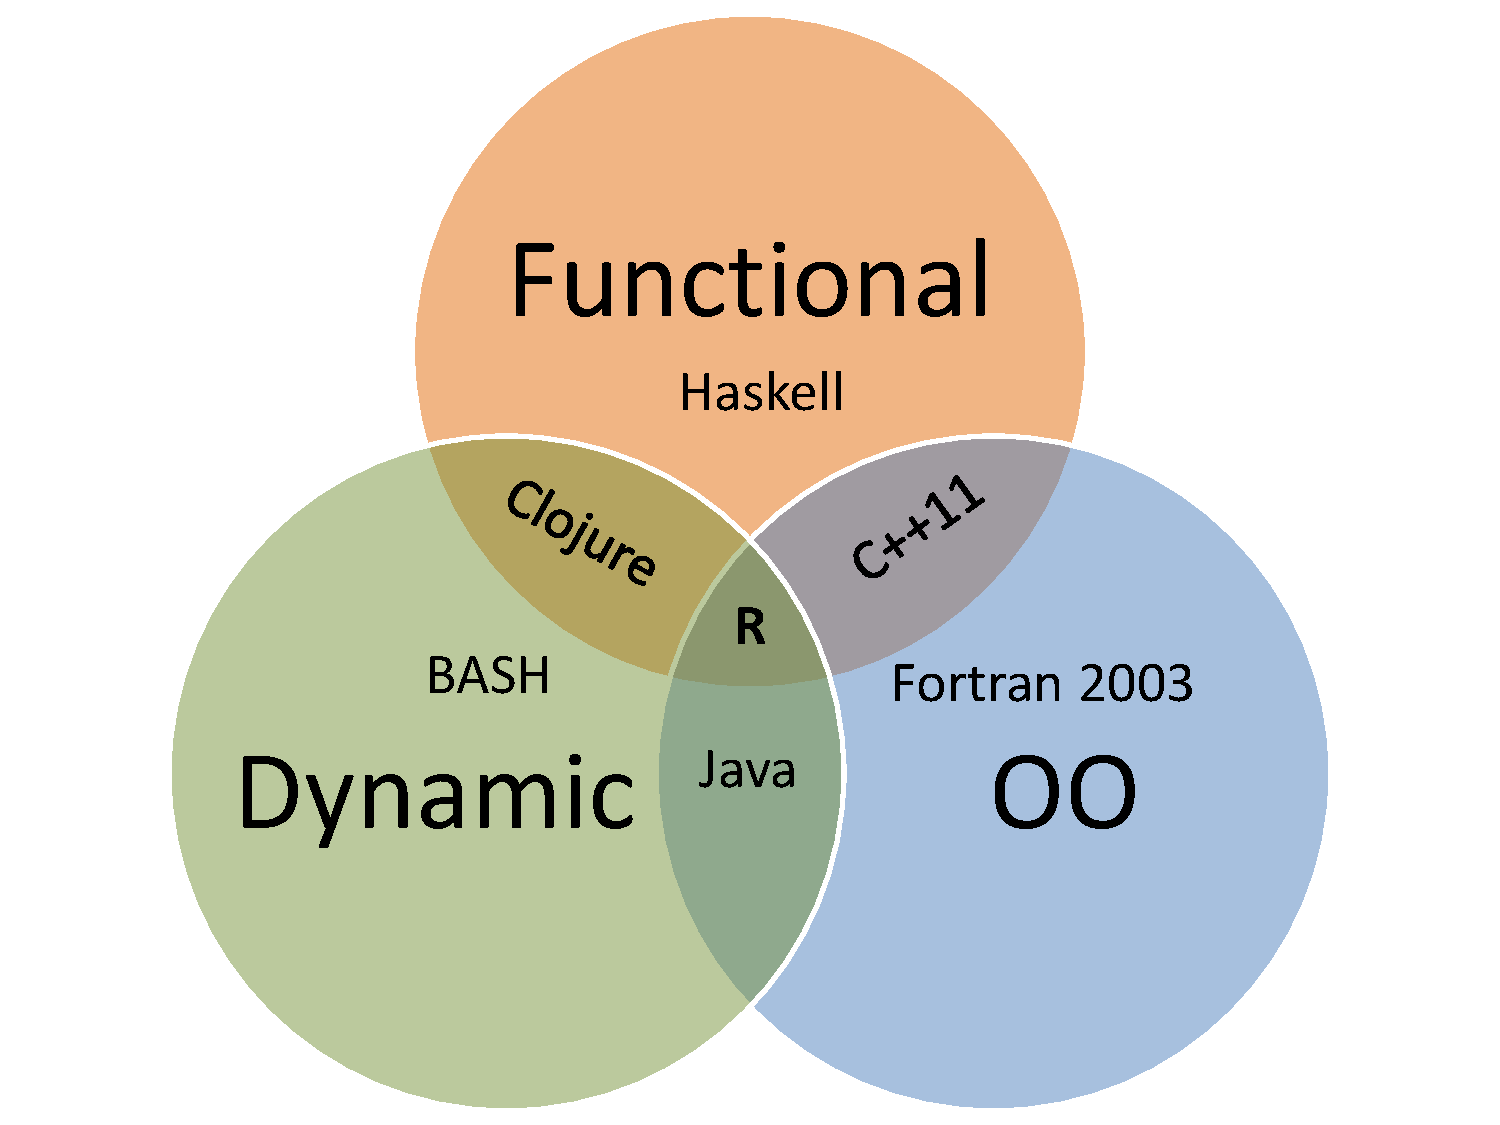
\includegraphics[scale=.35]{../common/pics/languages}
  \end{center}
  \end{block}
\end{frame}

\begin{frame}
  \begin{block}{Data Types}\pause
  \begin{itemize}[<+-|alert@+>]
    \item Storage:  logical, int, double, double complex, character
    \item Structures:  vector, matrix, array, list, dataframe
    \item Caveats:  (Logical) \code{TRUE}, \code{FALSE}, \code{NA}
  \end{itemize}
  For the remainder of the tutorial, we will restrict ourselves to real number 
matrix computations.
\end{block}
\end{frame}




\subsection{Syntax for Data Science}


\begin{frame}[fragile]
\begin{block}{High Level Syntax}\pause
\begin{lstlisting}
x <- matrix(rnorm(30), nrow=10)
x <- x[-1, 2:5]
x <- log(abs(x) + 1)
xtx <- t(x) %*% x
ans <- svd(solve(xtx))
\end{lstlisting}
\end{block}
\end{frame}


\begin{frame}
  \begin{block}{More than just a Matlab clone\dots}\pause
  \begin{itemize}[<+-|alert@+>]
    \item Data science (machine learning, statistics, data mining, \dots) is 
mostly matrix algebra.  \\[.2cm]
     So what about Matlab/Python/Julia/\dots ?
    \item Depends on your ``religion'' 
    \item As a \emph{data analysis} package, R is king.
  \end{itemize}
\end{block}
\end{frame}



\begin{frame}[fragile]
\begin{block}{High Level Syntax \emph{for Data}}\pause
\begin{lstlisting}
pca <- prcomp(x, retx=TRUE, scale=TRUE)
prop_var <- cumsum(pca$sdev)/sum(pca$sdev)
i <- min(which(prop_var > 0.9)) - 1

y <- pca$x[, 1:i]
\end{lstlisting}
\end{block}
\end{frame}

















\section{Parallel Hardware and R}

\hidenum
\begin{frame}[noframenumbering]
\frametitle{Contents}
 \tableofcontents[currentsection,hideothersubsections,sectionstyle=show/hide]
\end{frame}
\shownum

\subsection{Parallel Hardware}

% \begin{frame}
% \begin{block}{A}
%   
% \end{block}
% \end{frame}


\begin{frame}
\begin{block}{Three Basic Flavors of Hardware}
    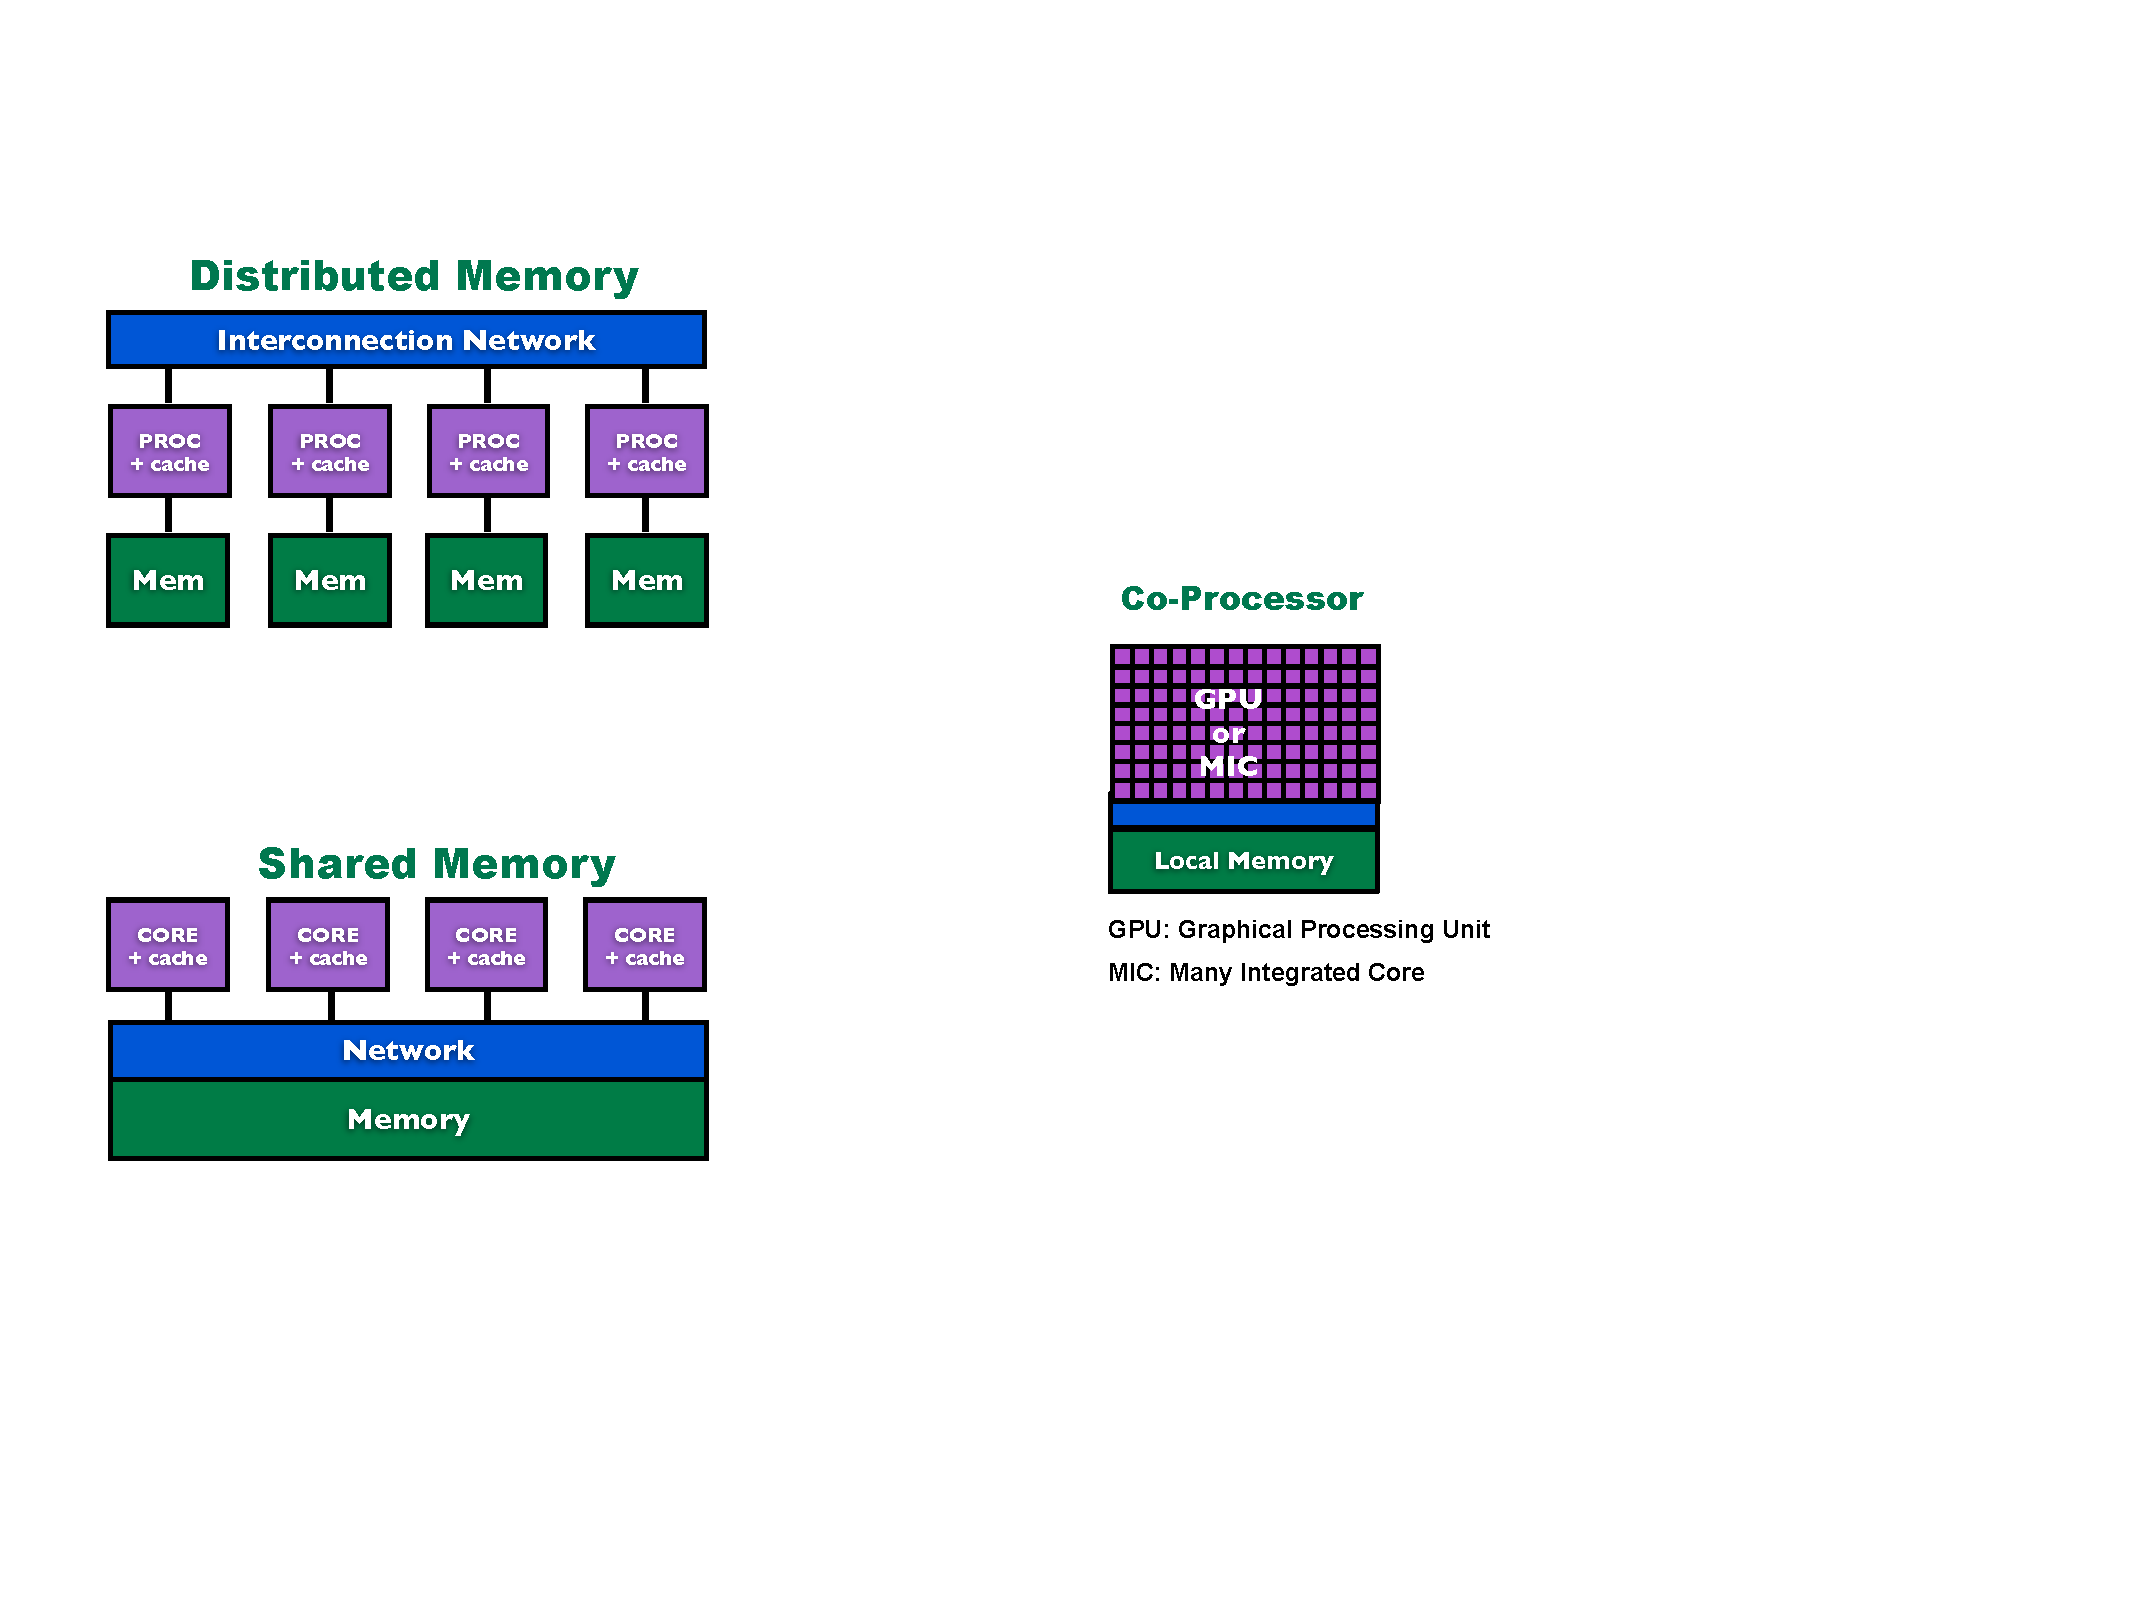
\includegraphics[width=0.95\textwidth]{../common/pics/ParallelHardware1.pdf}
\end{block}
\end{frame}

\begin{frame}
\begin{block}{Your Laptop or Desktop}
    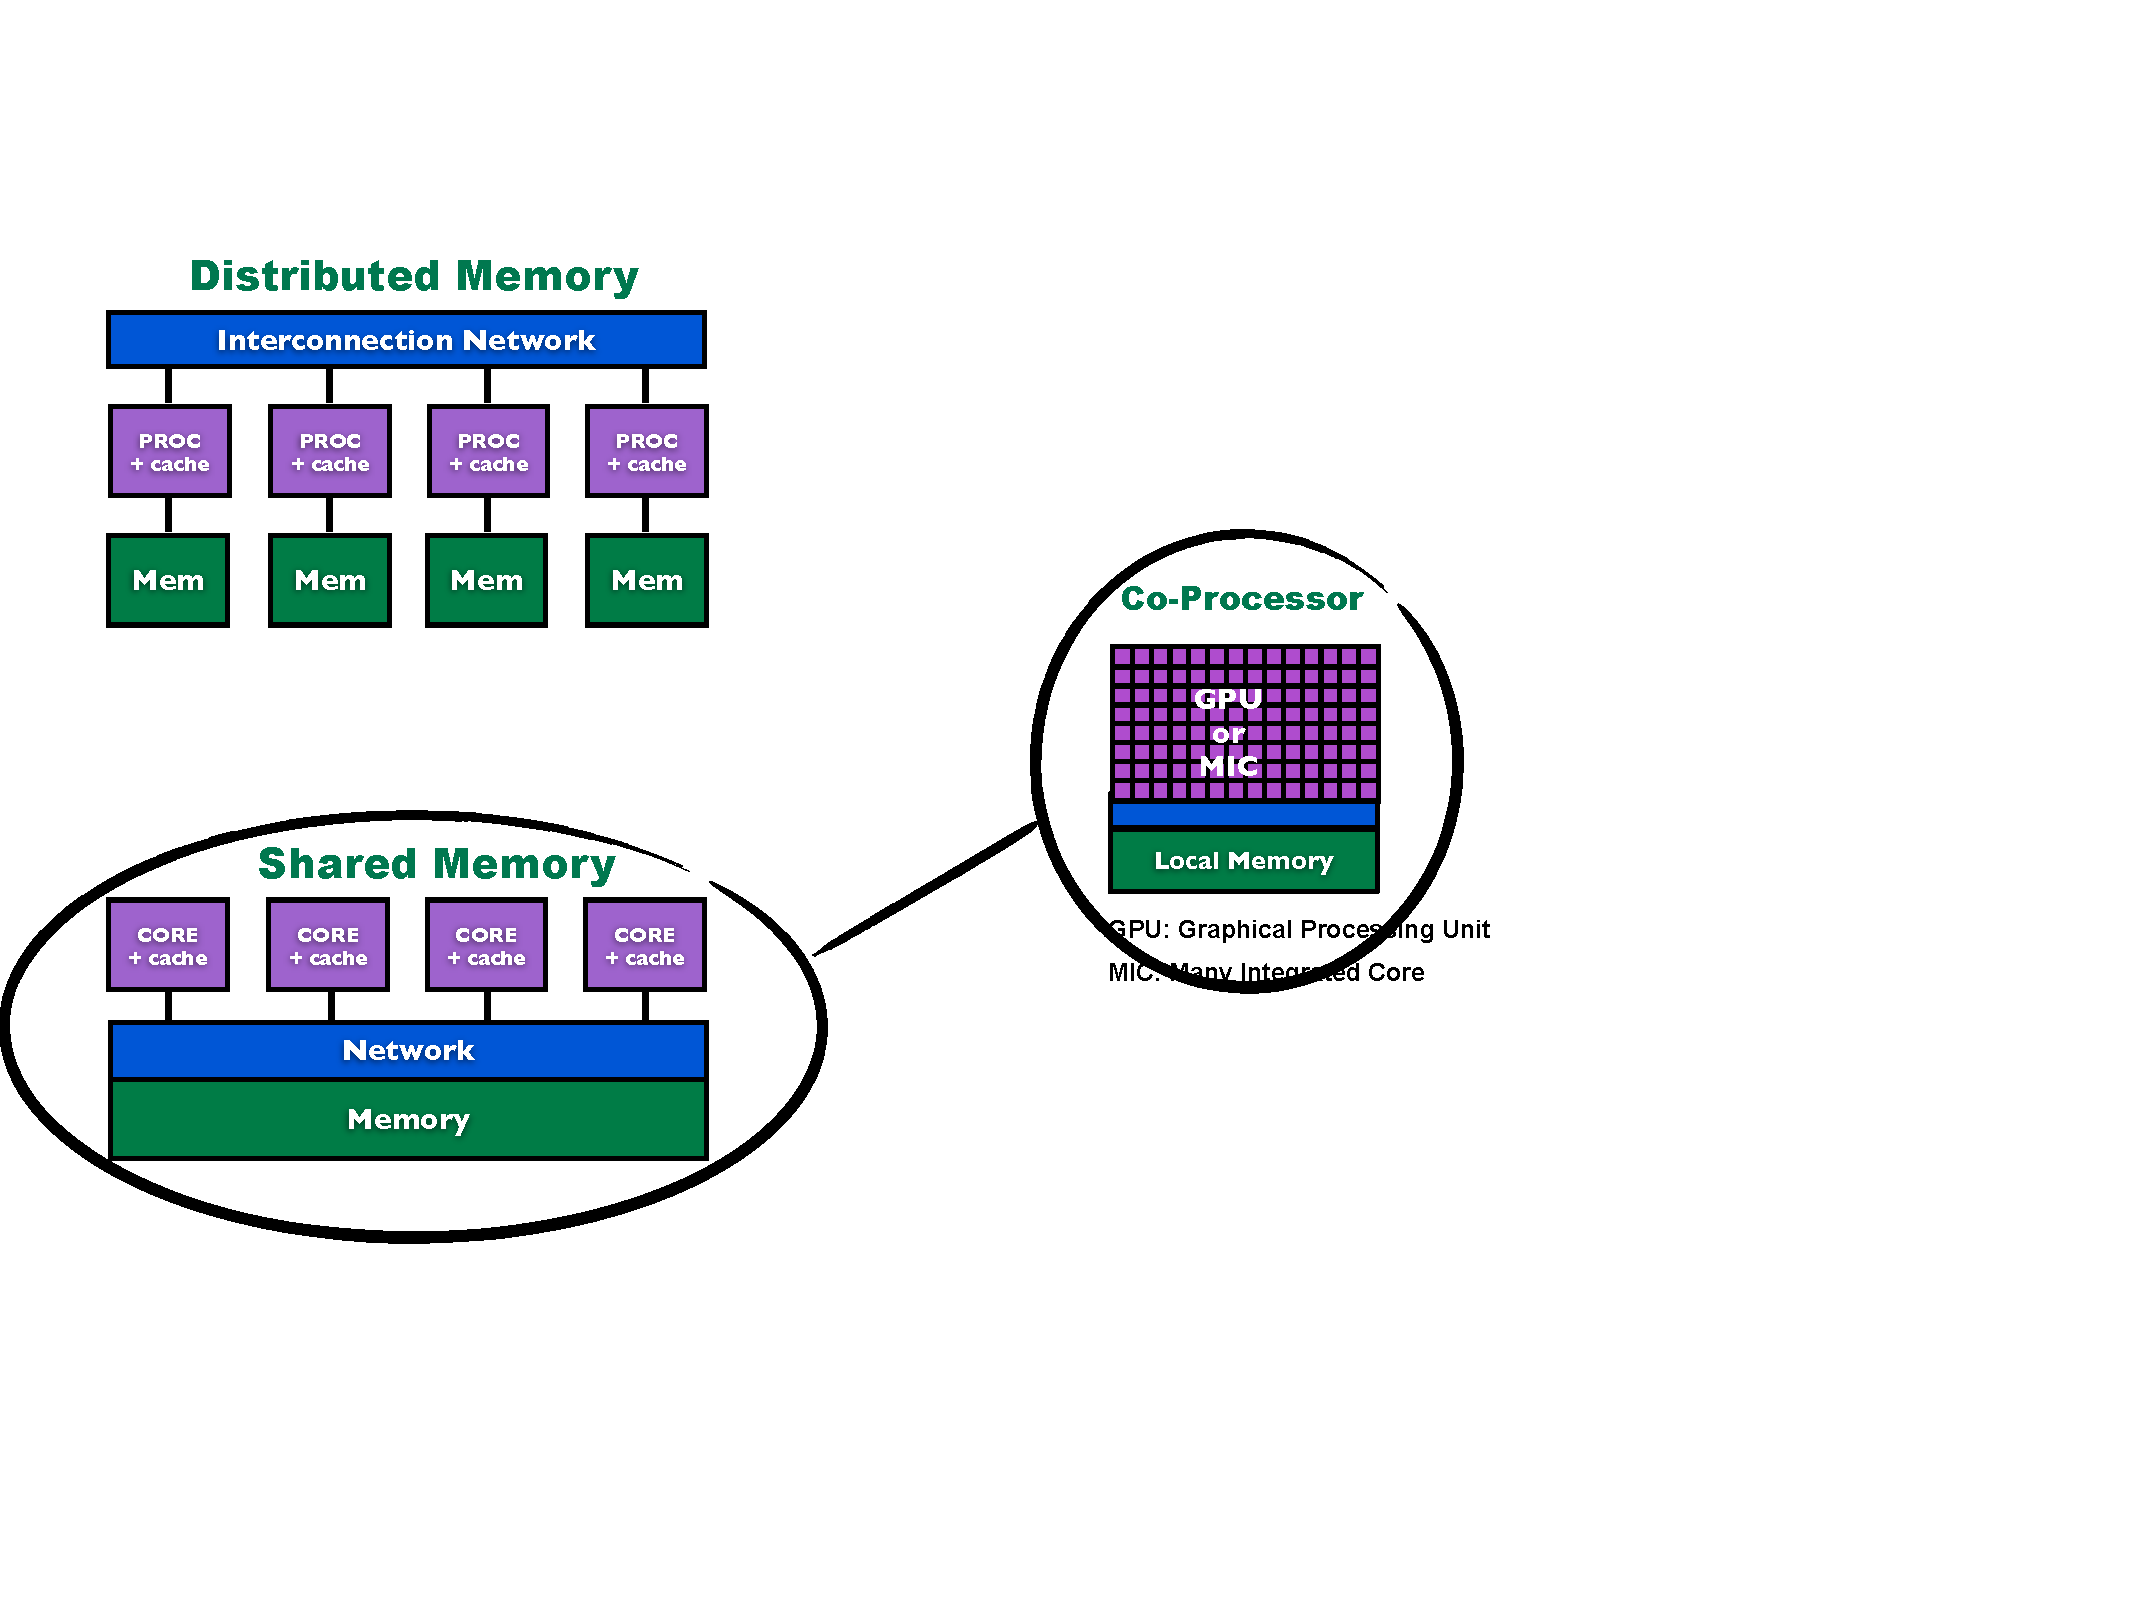
\includegraphics[width=0.95\textwidth]{../common/pics/ParallelHardware2.pdf}
\end{block}
\end{frame}

\begin{frame}
\begin{block}{A Server or Cluster}
    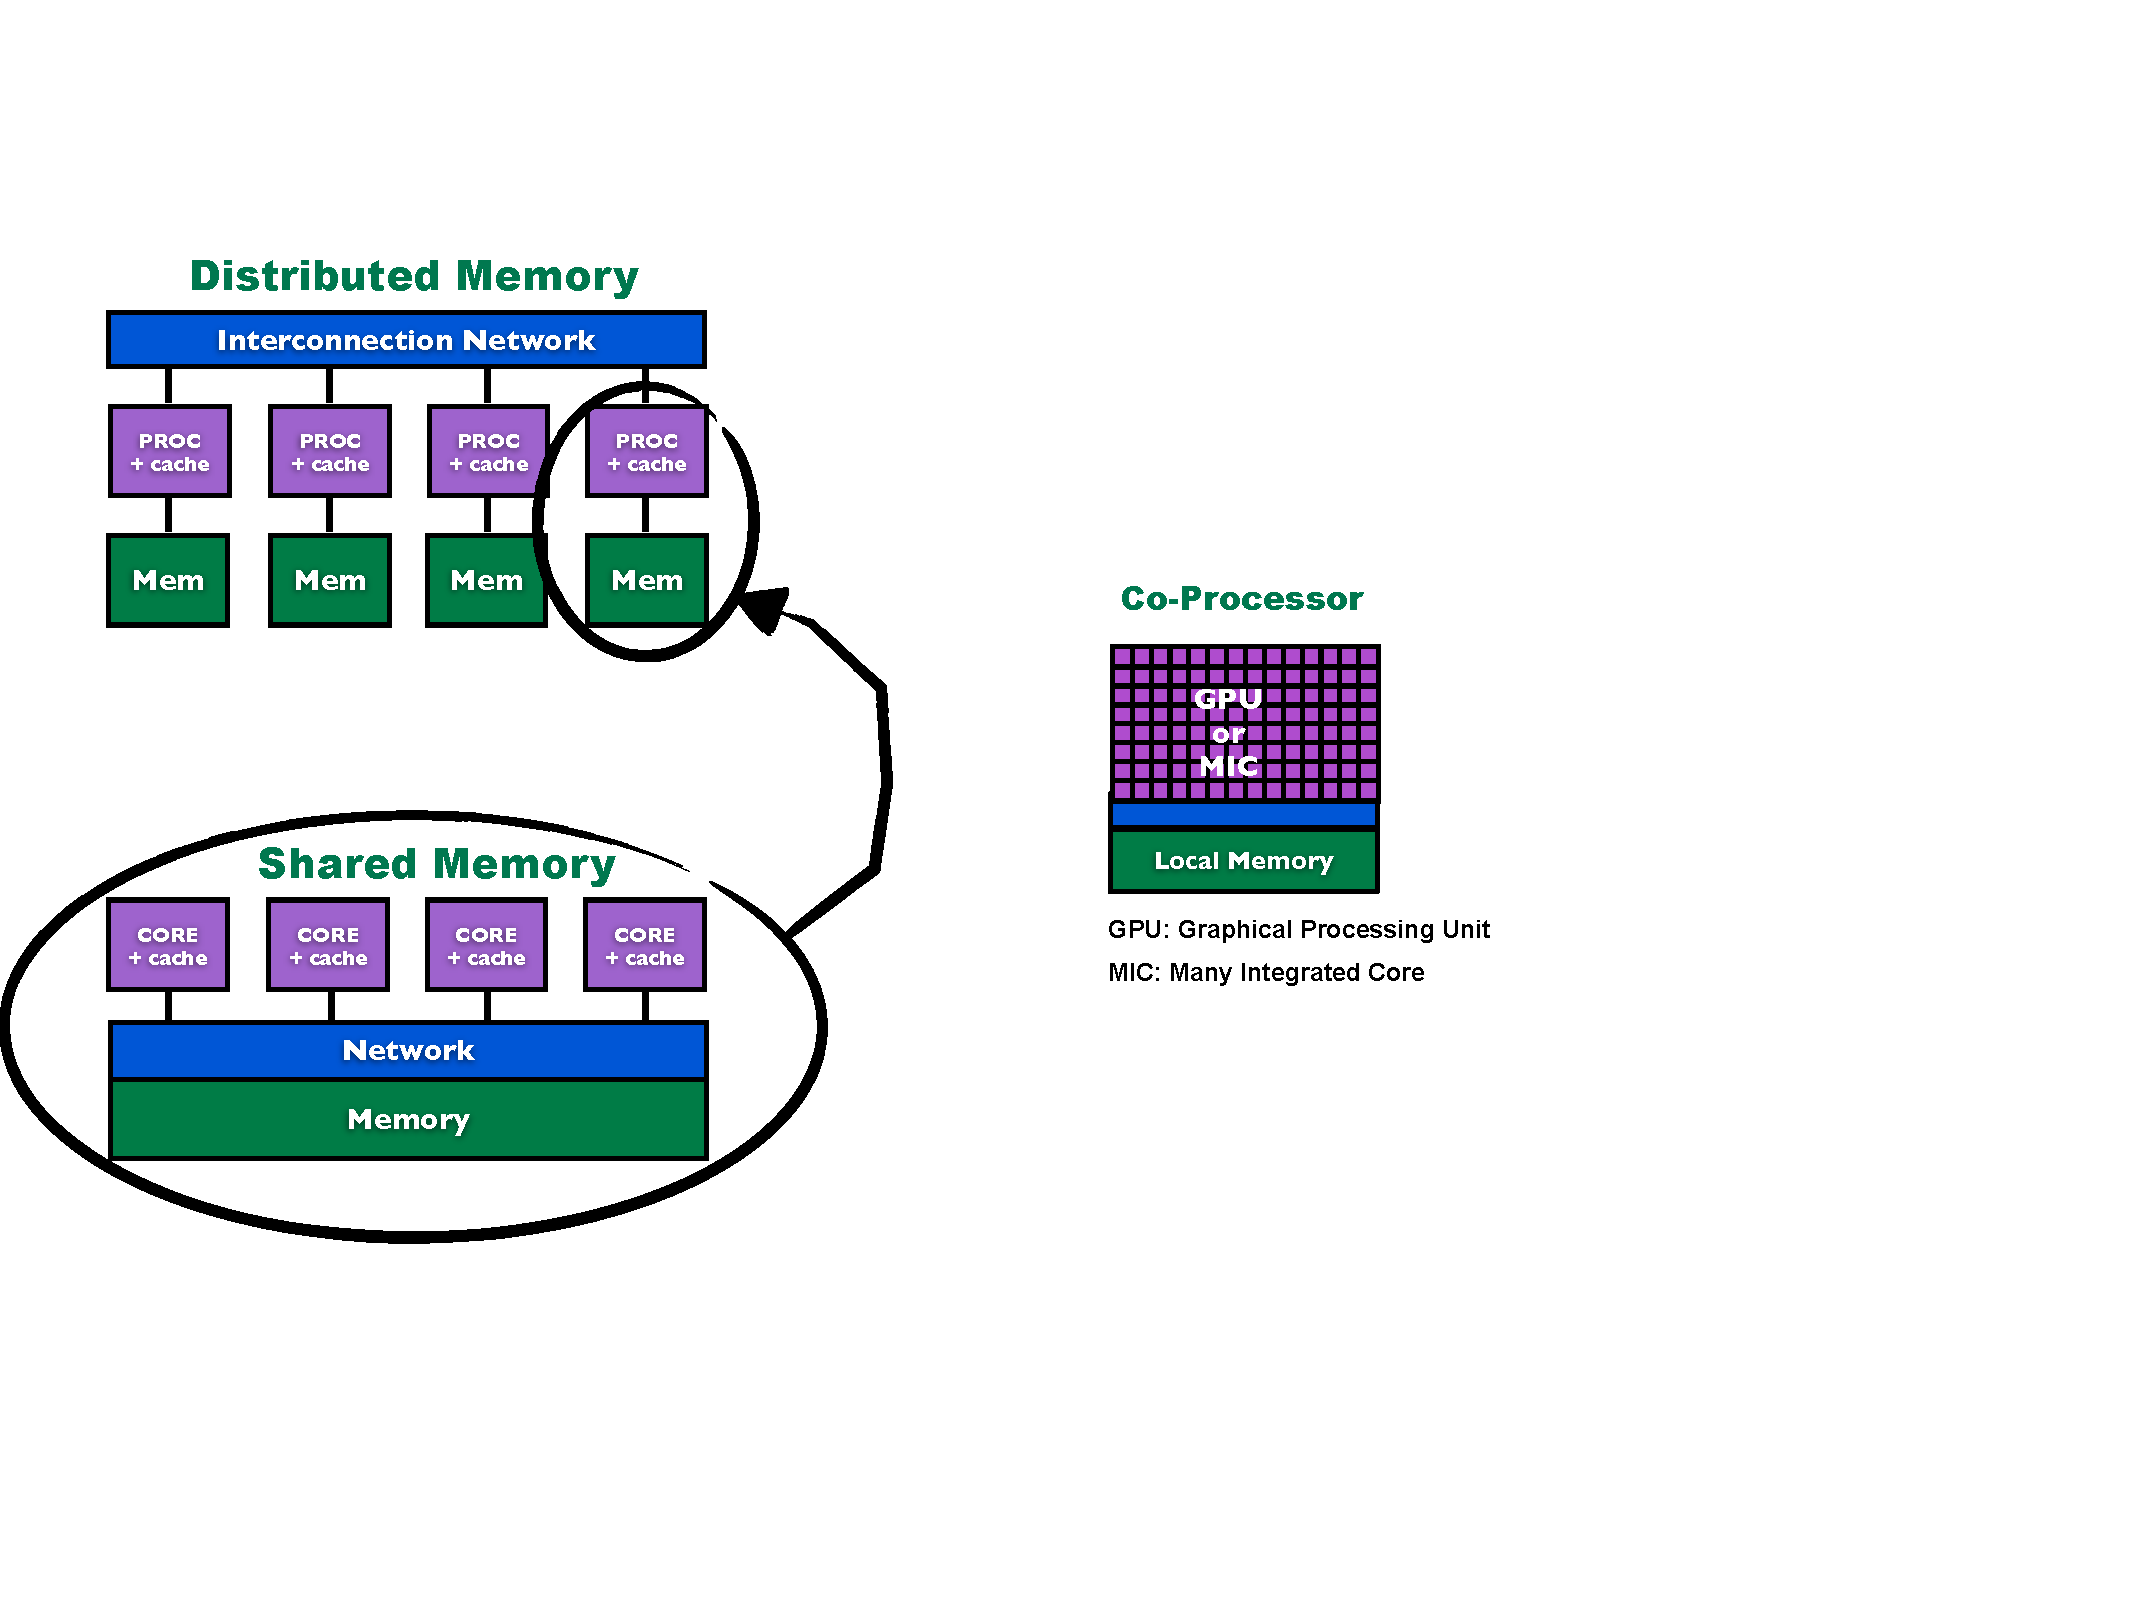
\includegraphics[width=0.95\textwidth]{../common/pics/ParallelHardware3.pdf}
\end{block}
\end{frame}

\begin{frame}
\begin{block}{Server to Supercomputer}
    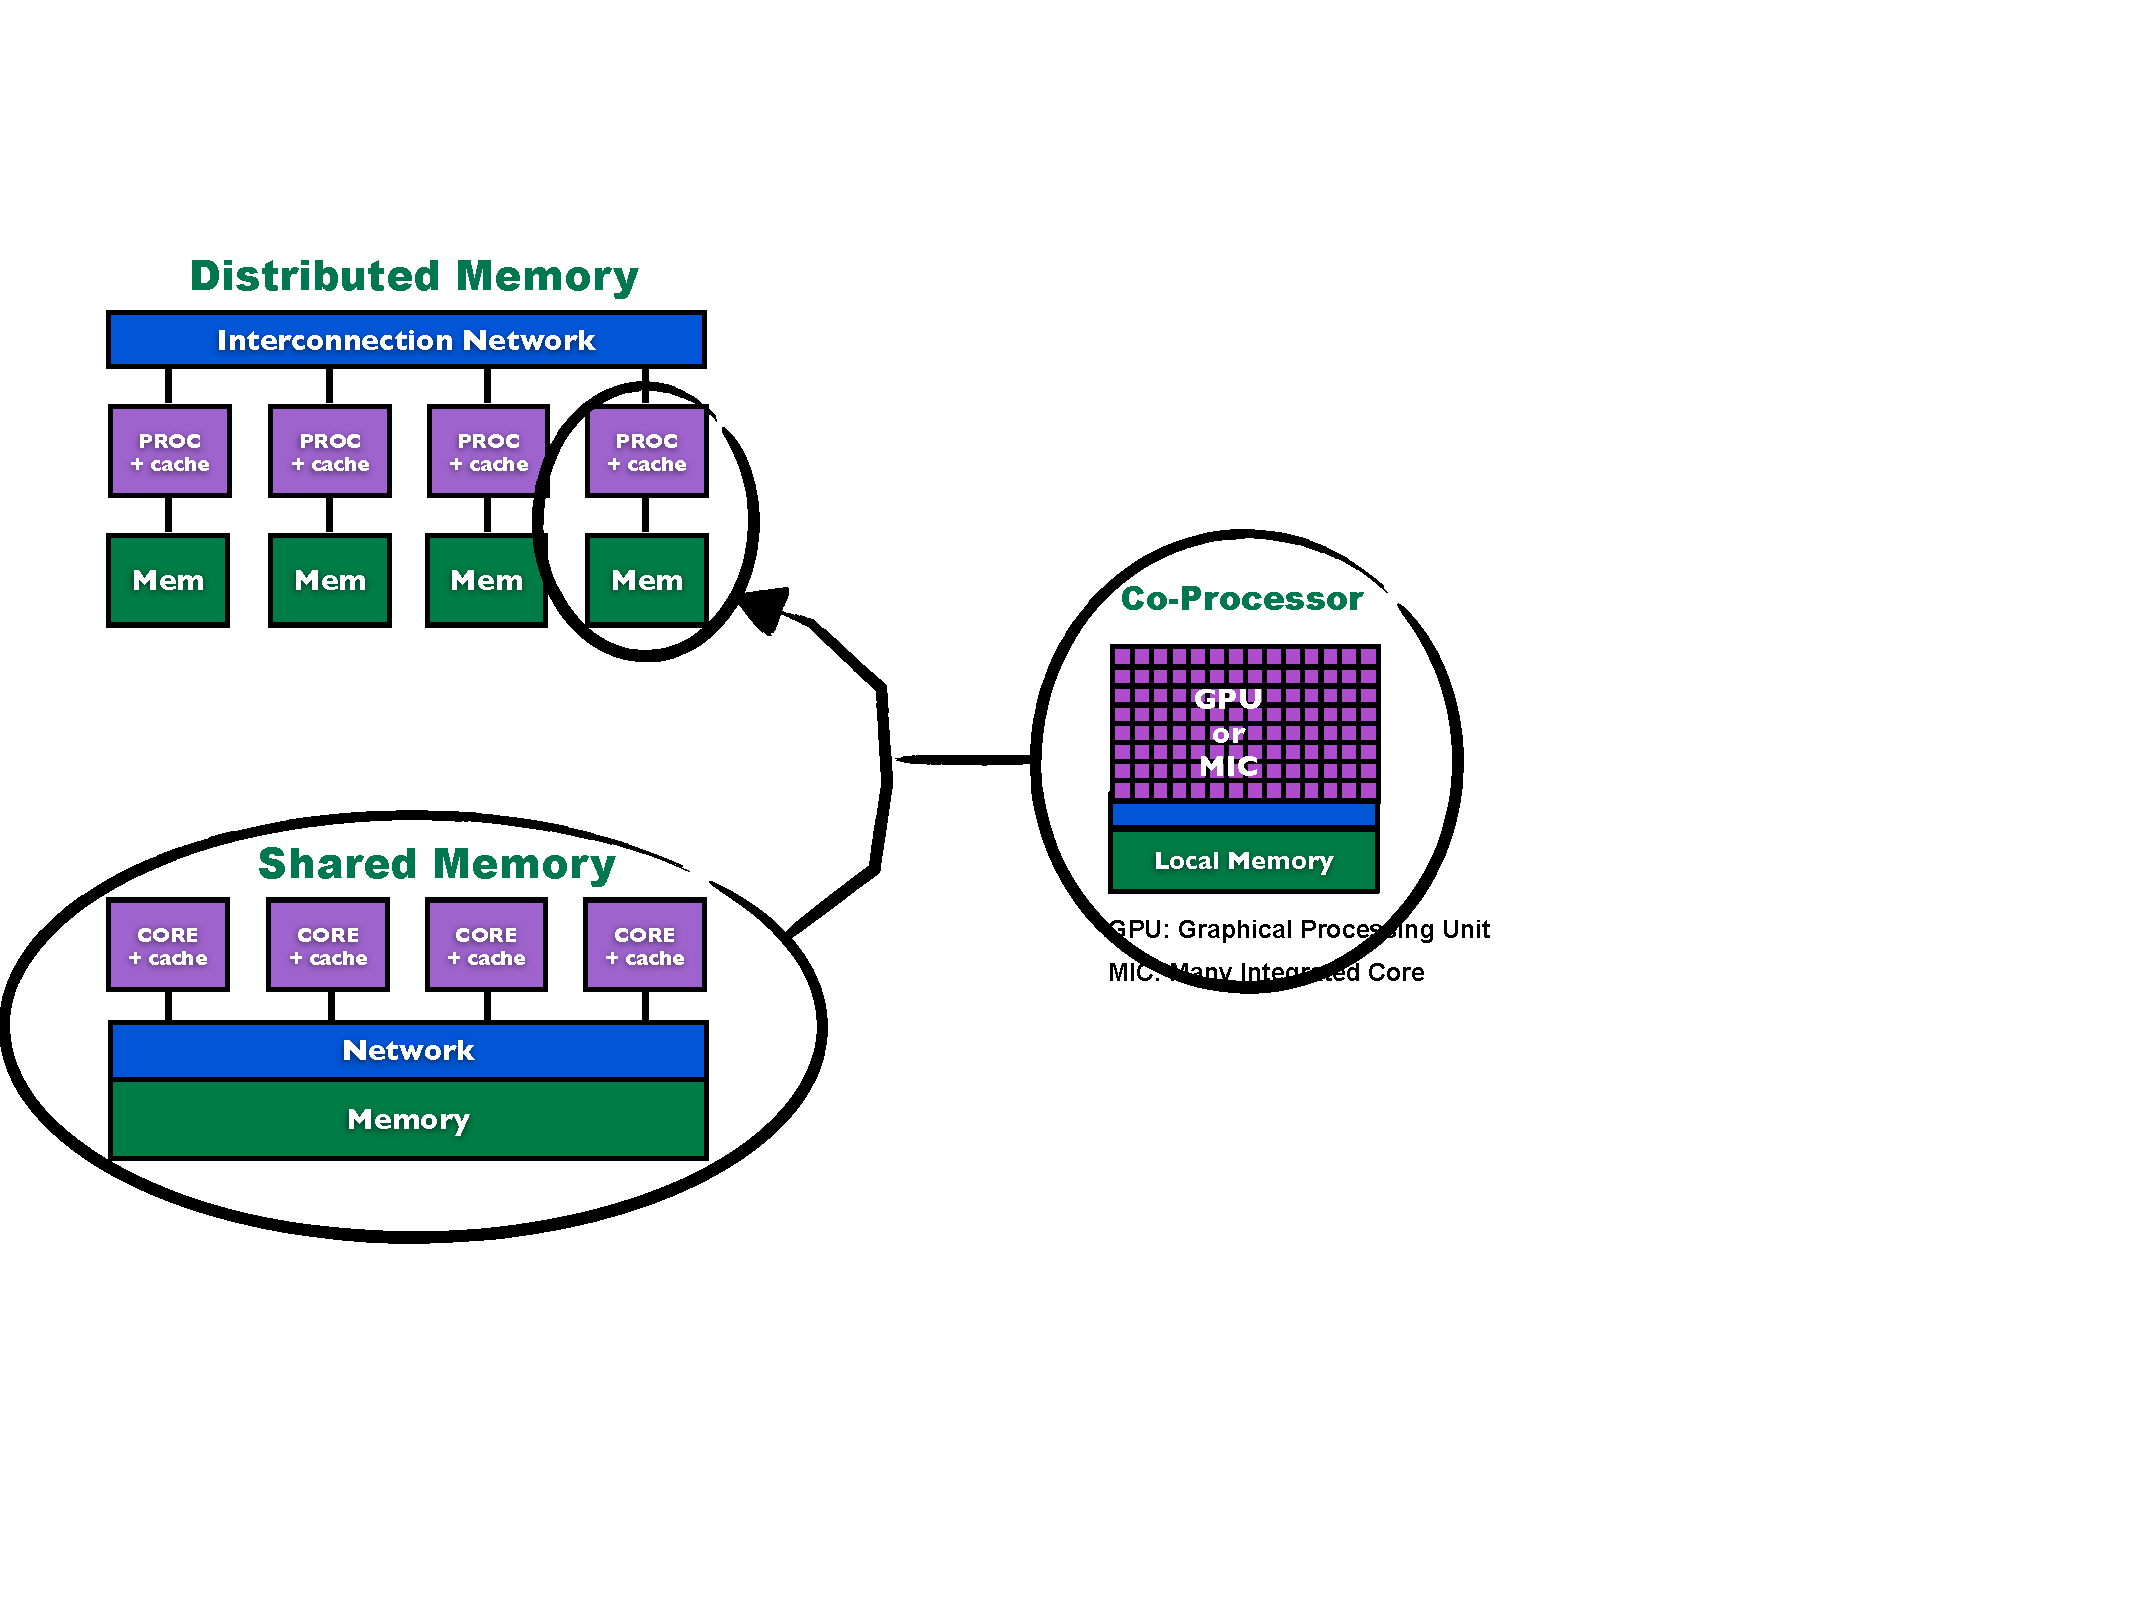
\includegraphics[width=0.95\textwidth]{../common/pics/ParallelHardware4.pdf}
\end{block}
\end{frame}

\begin{frame}
\begin{block}{Knowing the Right Words}
    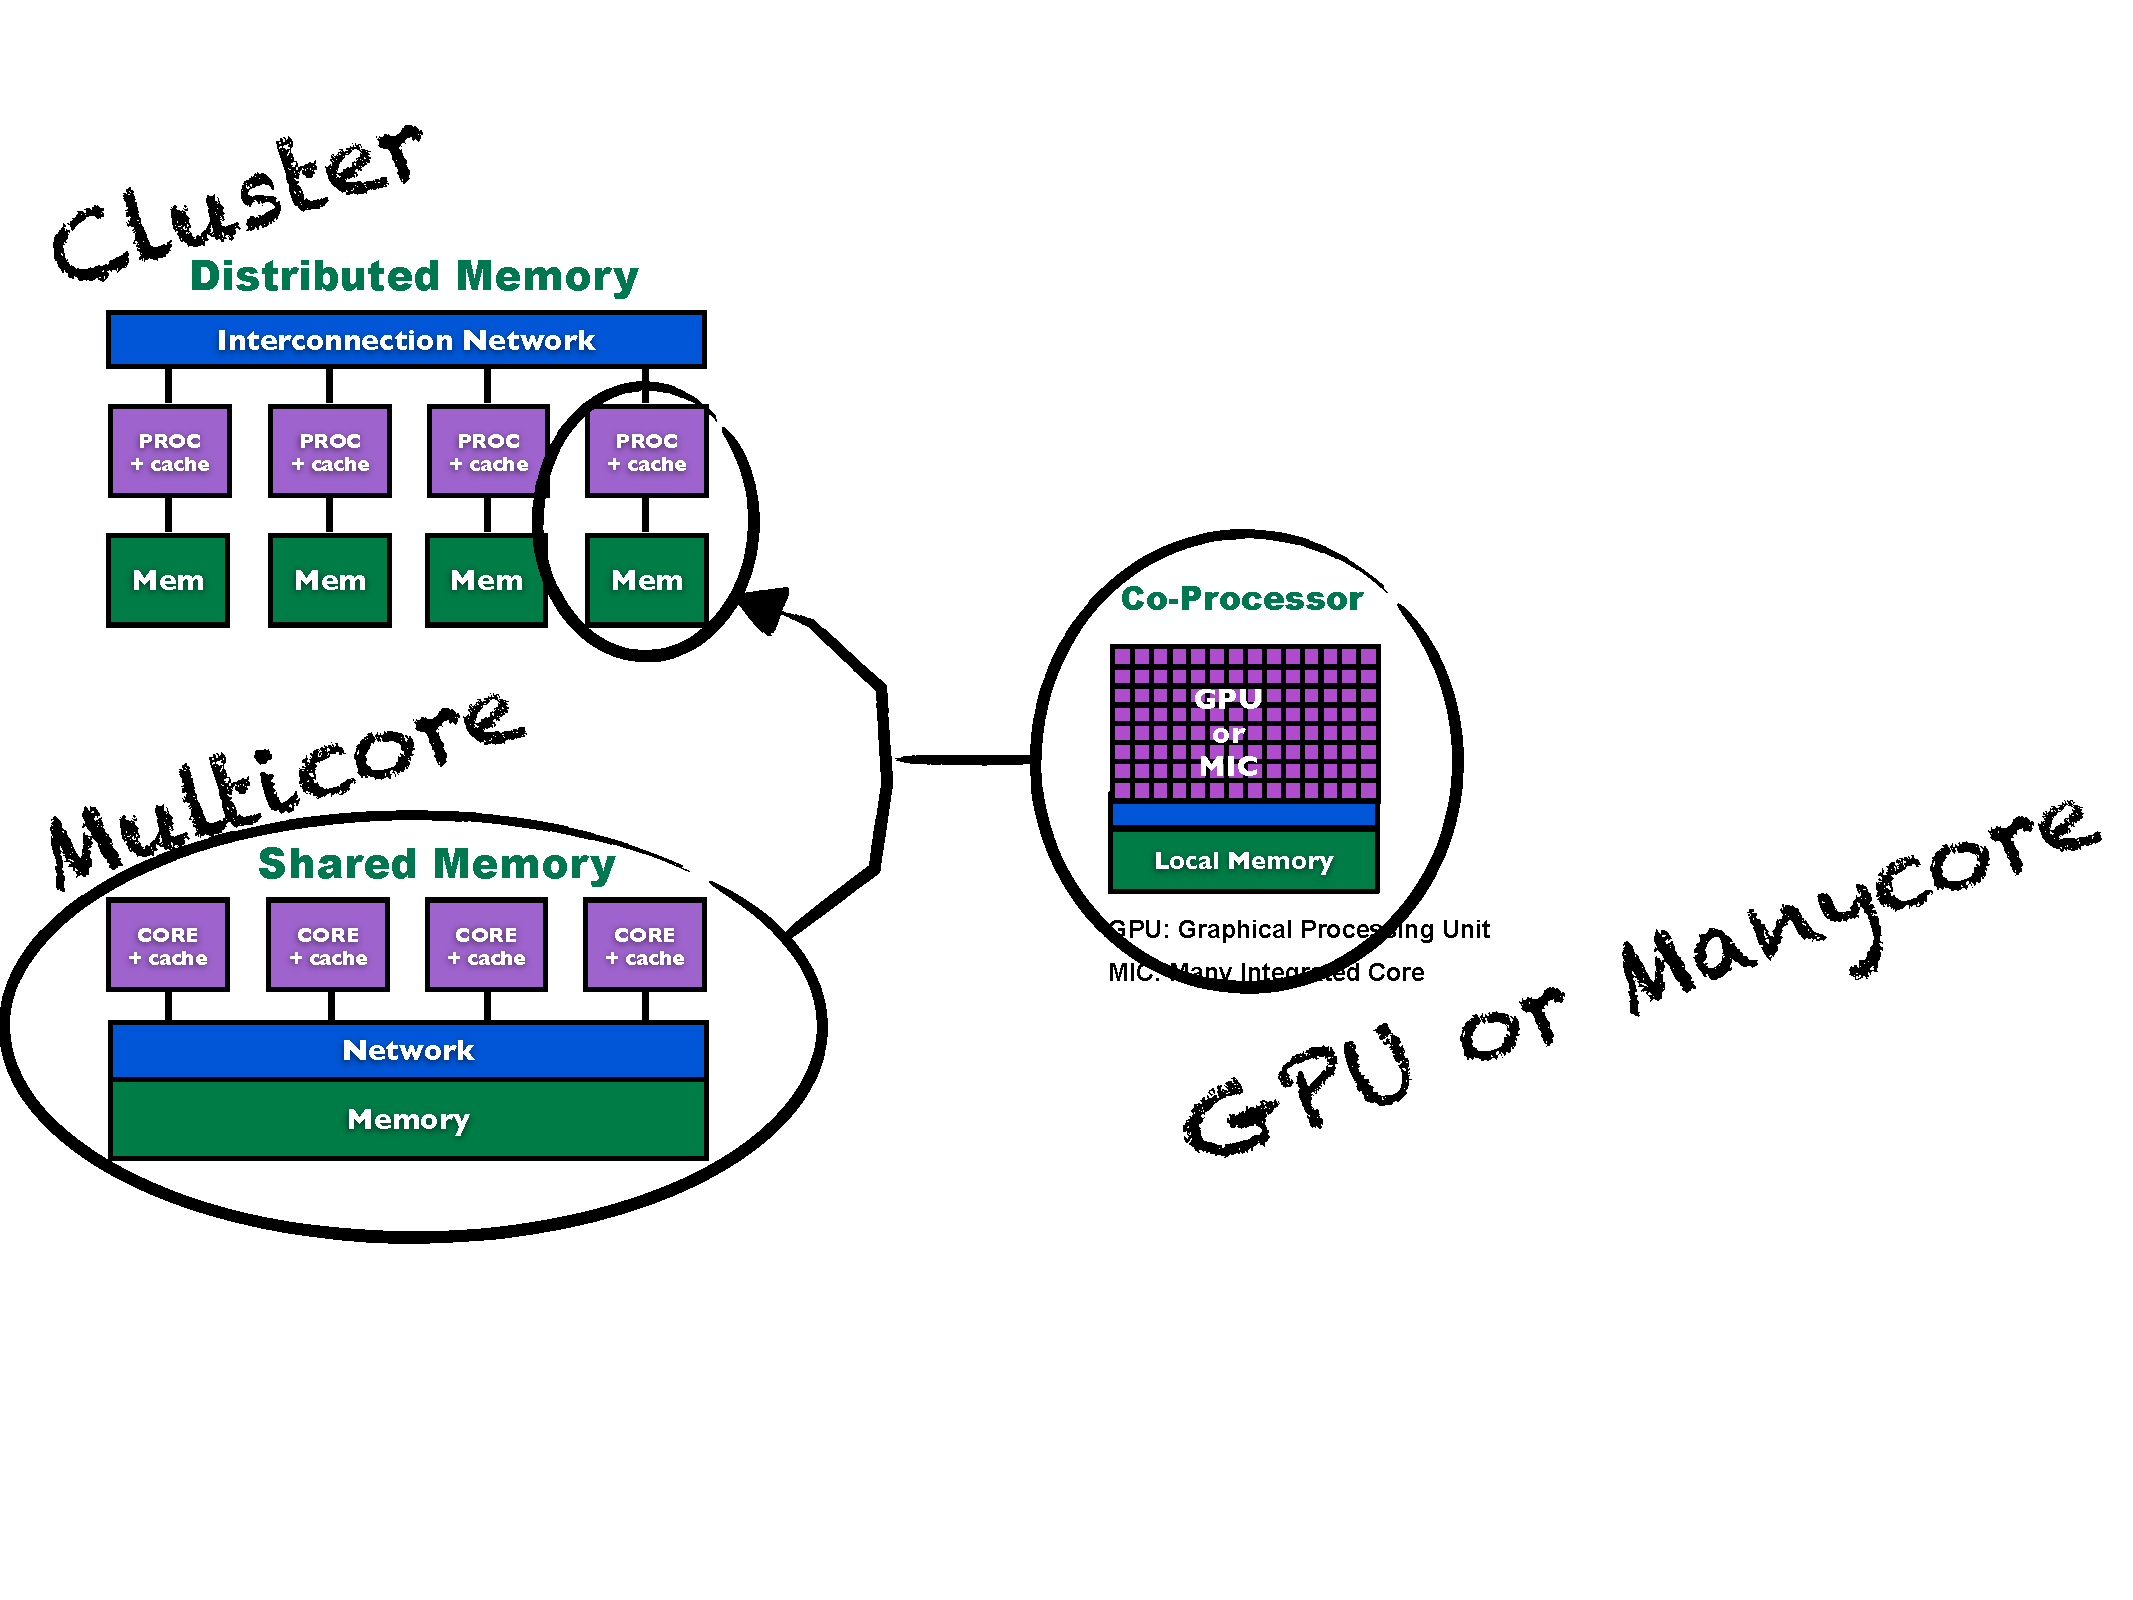
\includegraphics[width=0.95\textwidth]{../common/pics/ParallelHardware5.pdf}
\end{block}
\end{frame}

\begin{frame}
\begin{block}{``Native'' Programming Models and Tools}
    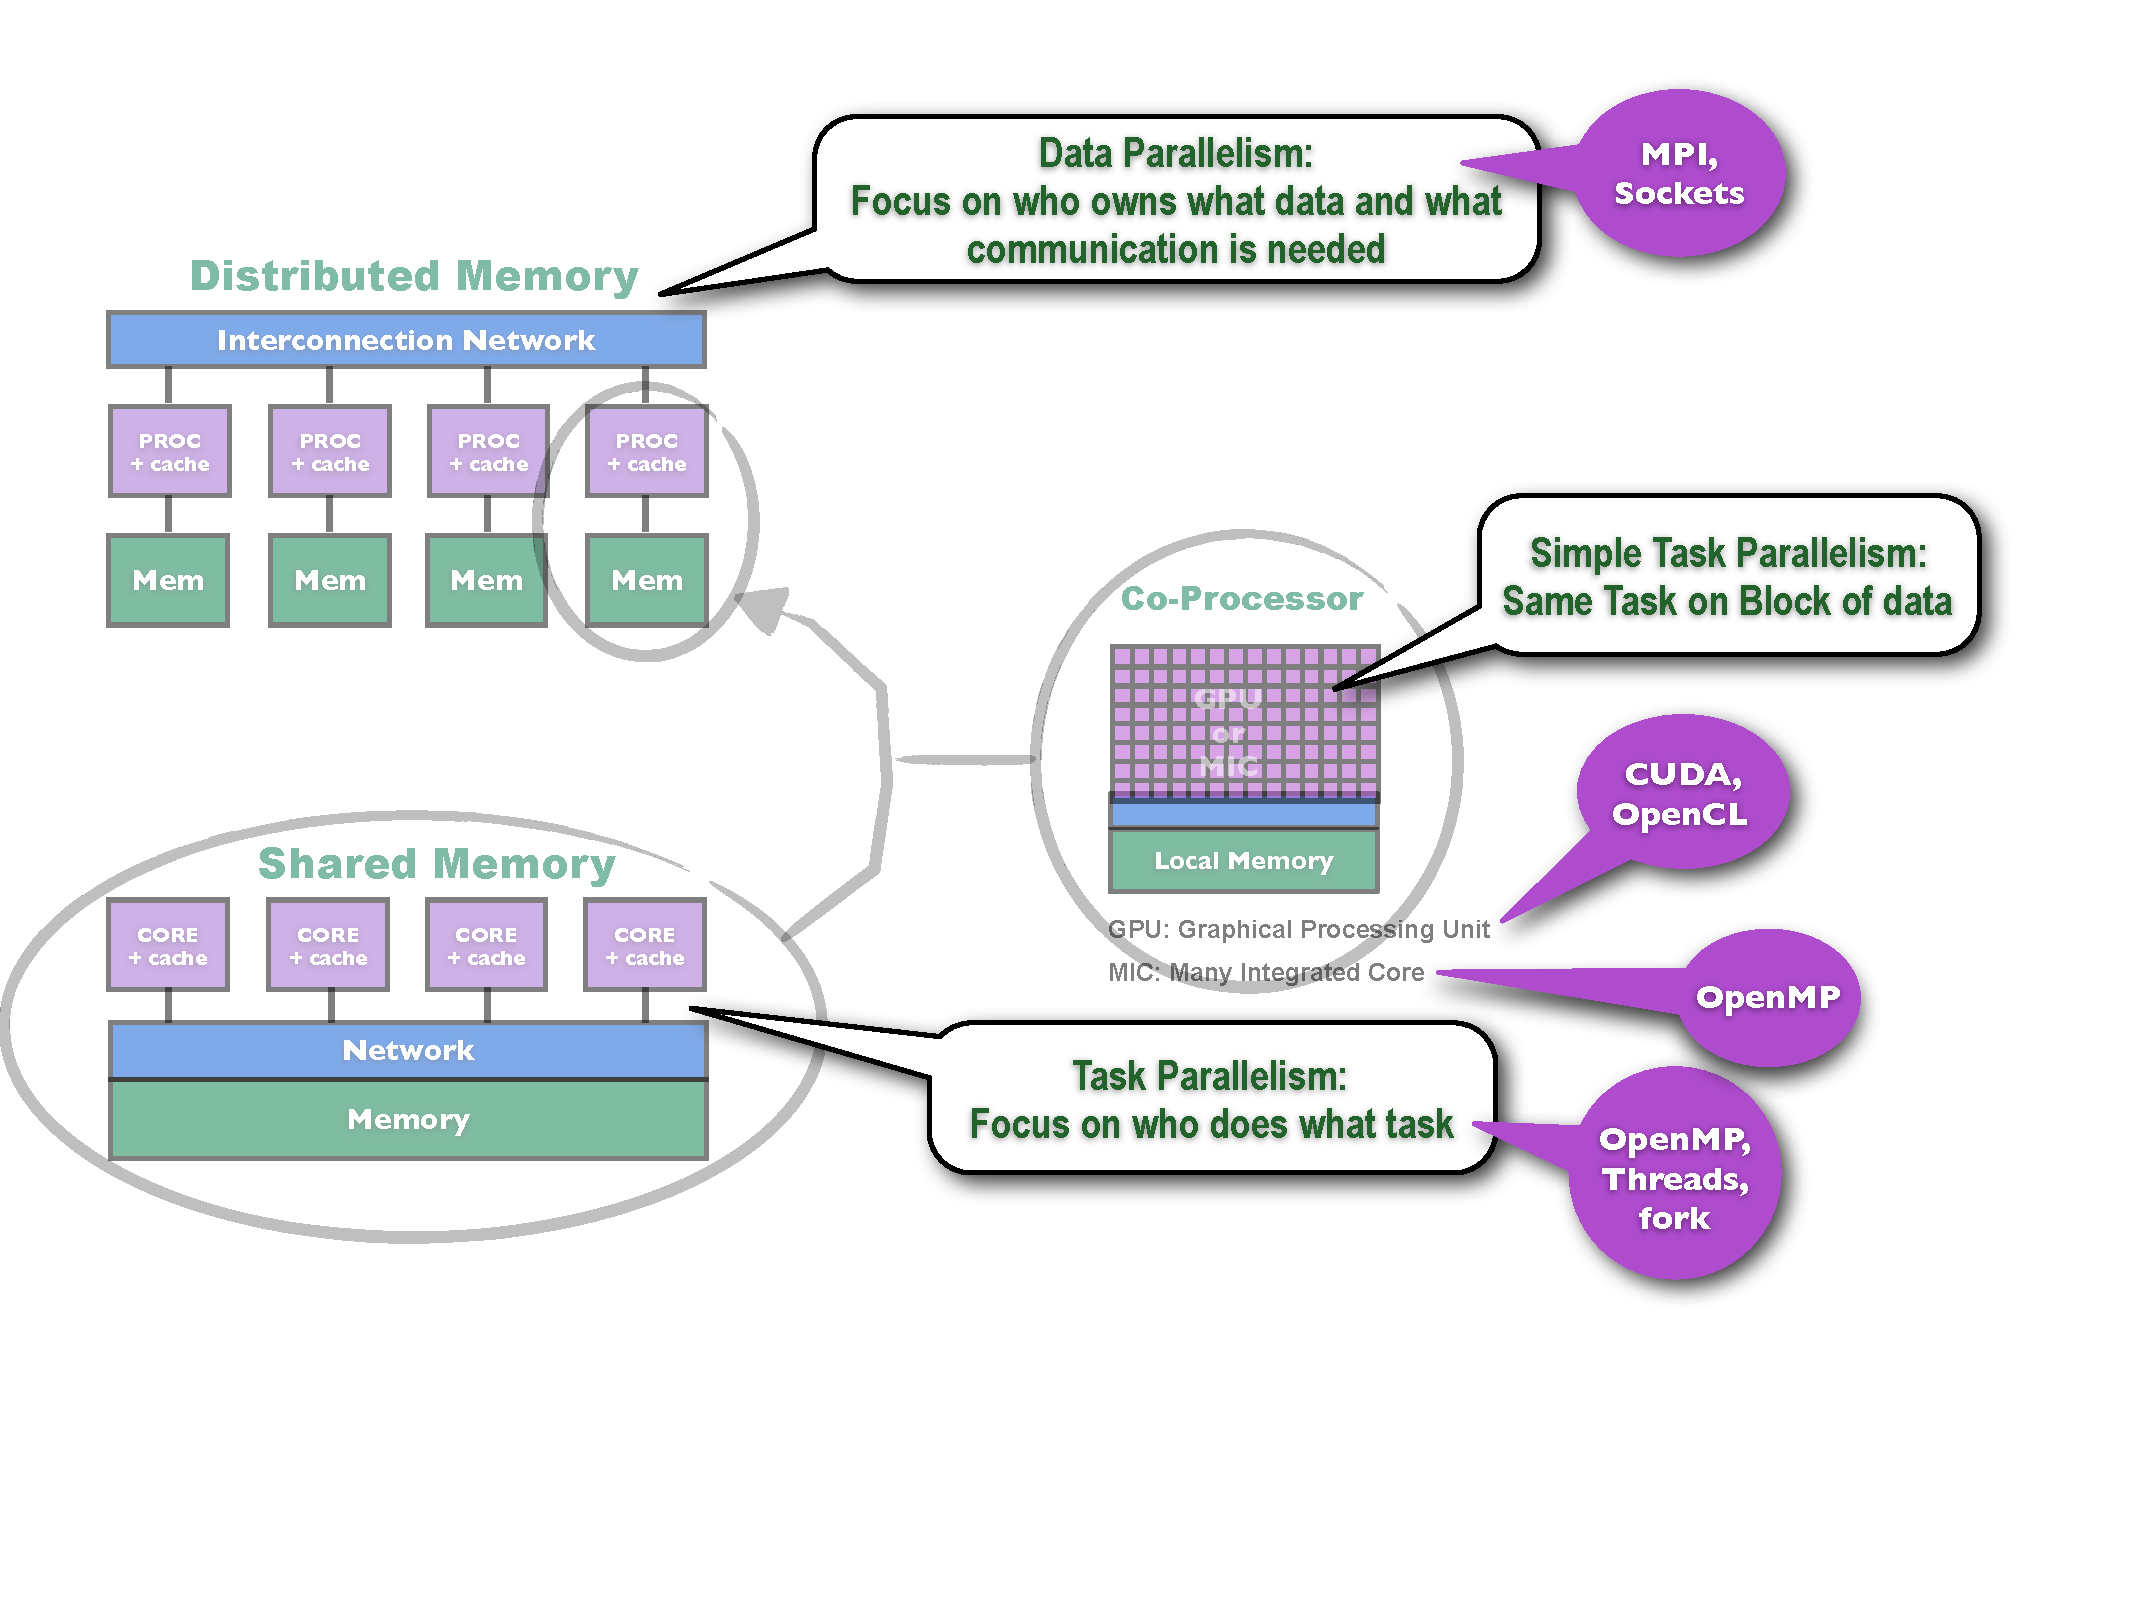
\includegraphics[width=0.95\textwidth]{../common/pics/ParallelHardware6.pdf}
\end{block}
\end{frame}

\subsection{R Interfaces to Parallel Hardware}

\begin{frame}
\begin{block}{R Interfaces to Native Tools}
    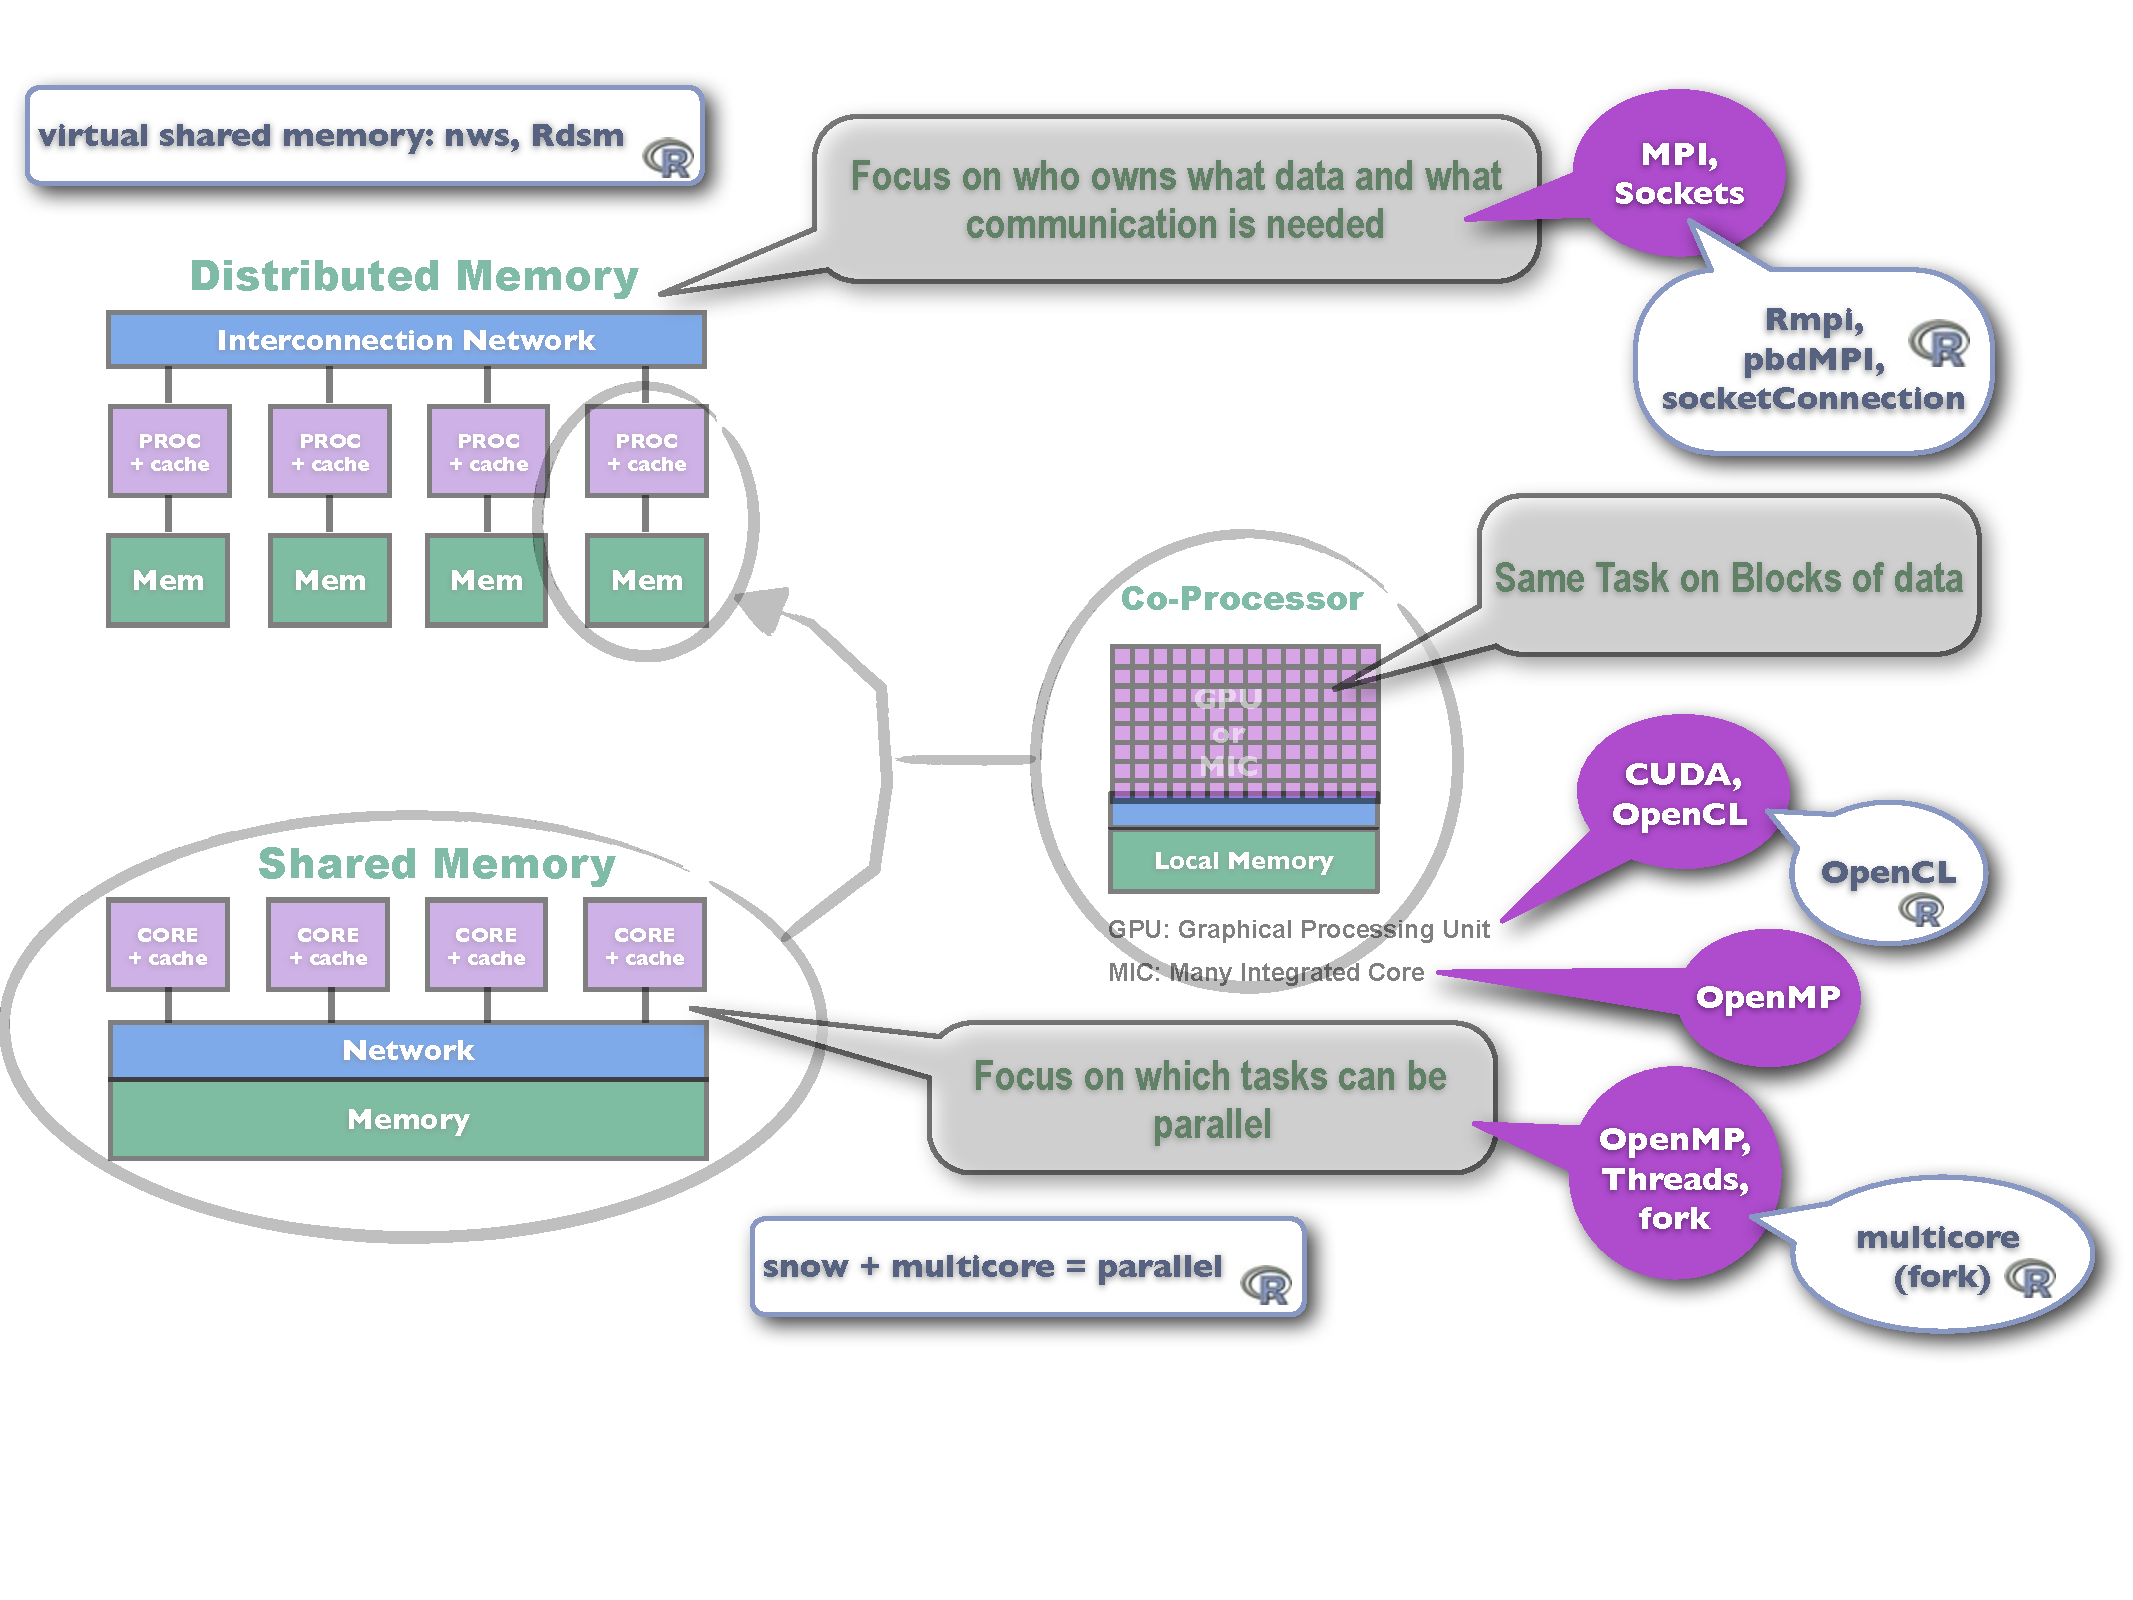
\includegraphics[width=0.95\textwidth]{../common/pics/ParallelHardware7.pdf}
\end{block}
\end{frame}

\begin{frame}
\begin{block}{30+ Years of Parallel Computing Research}
    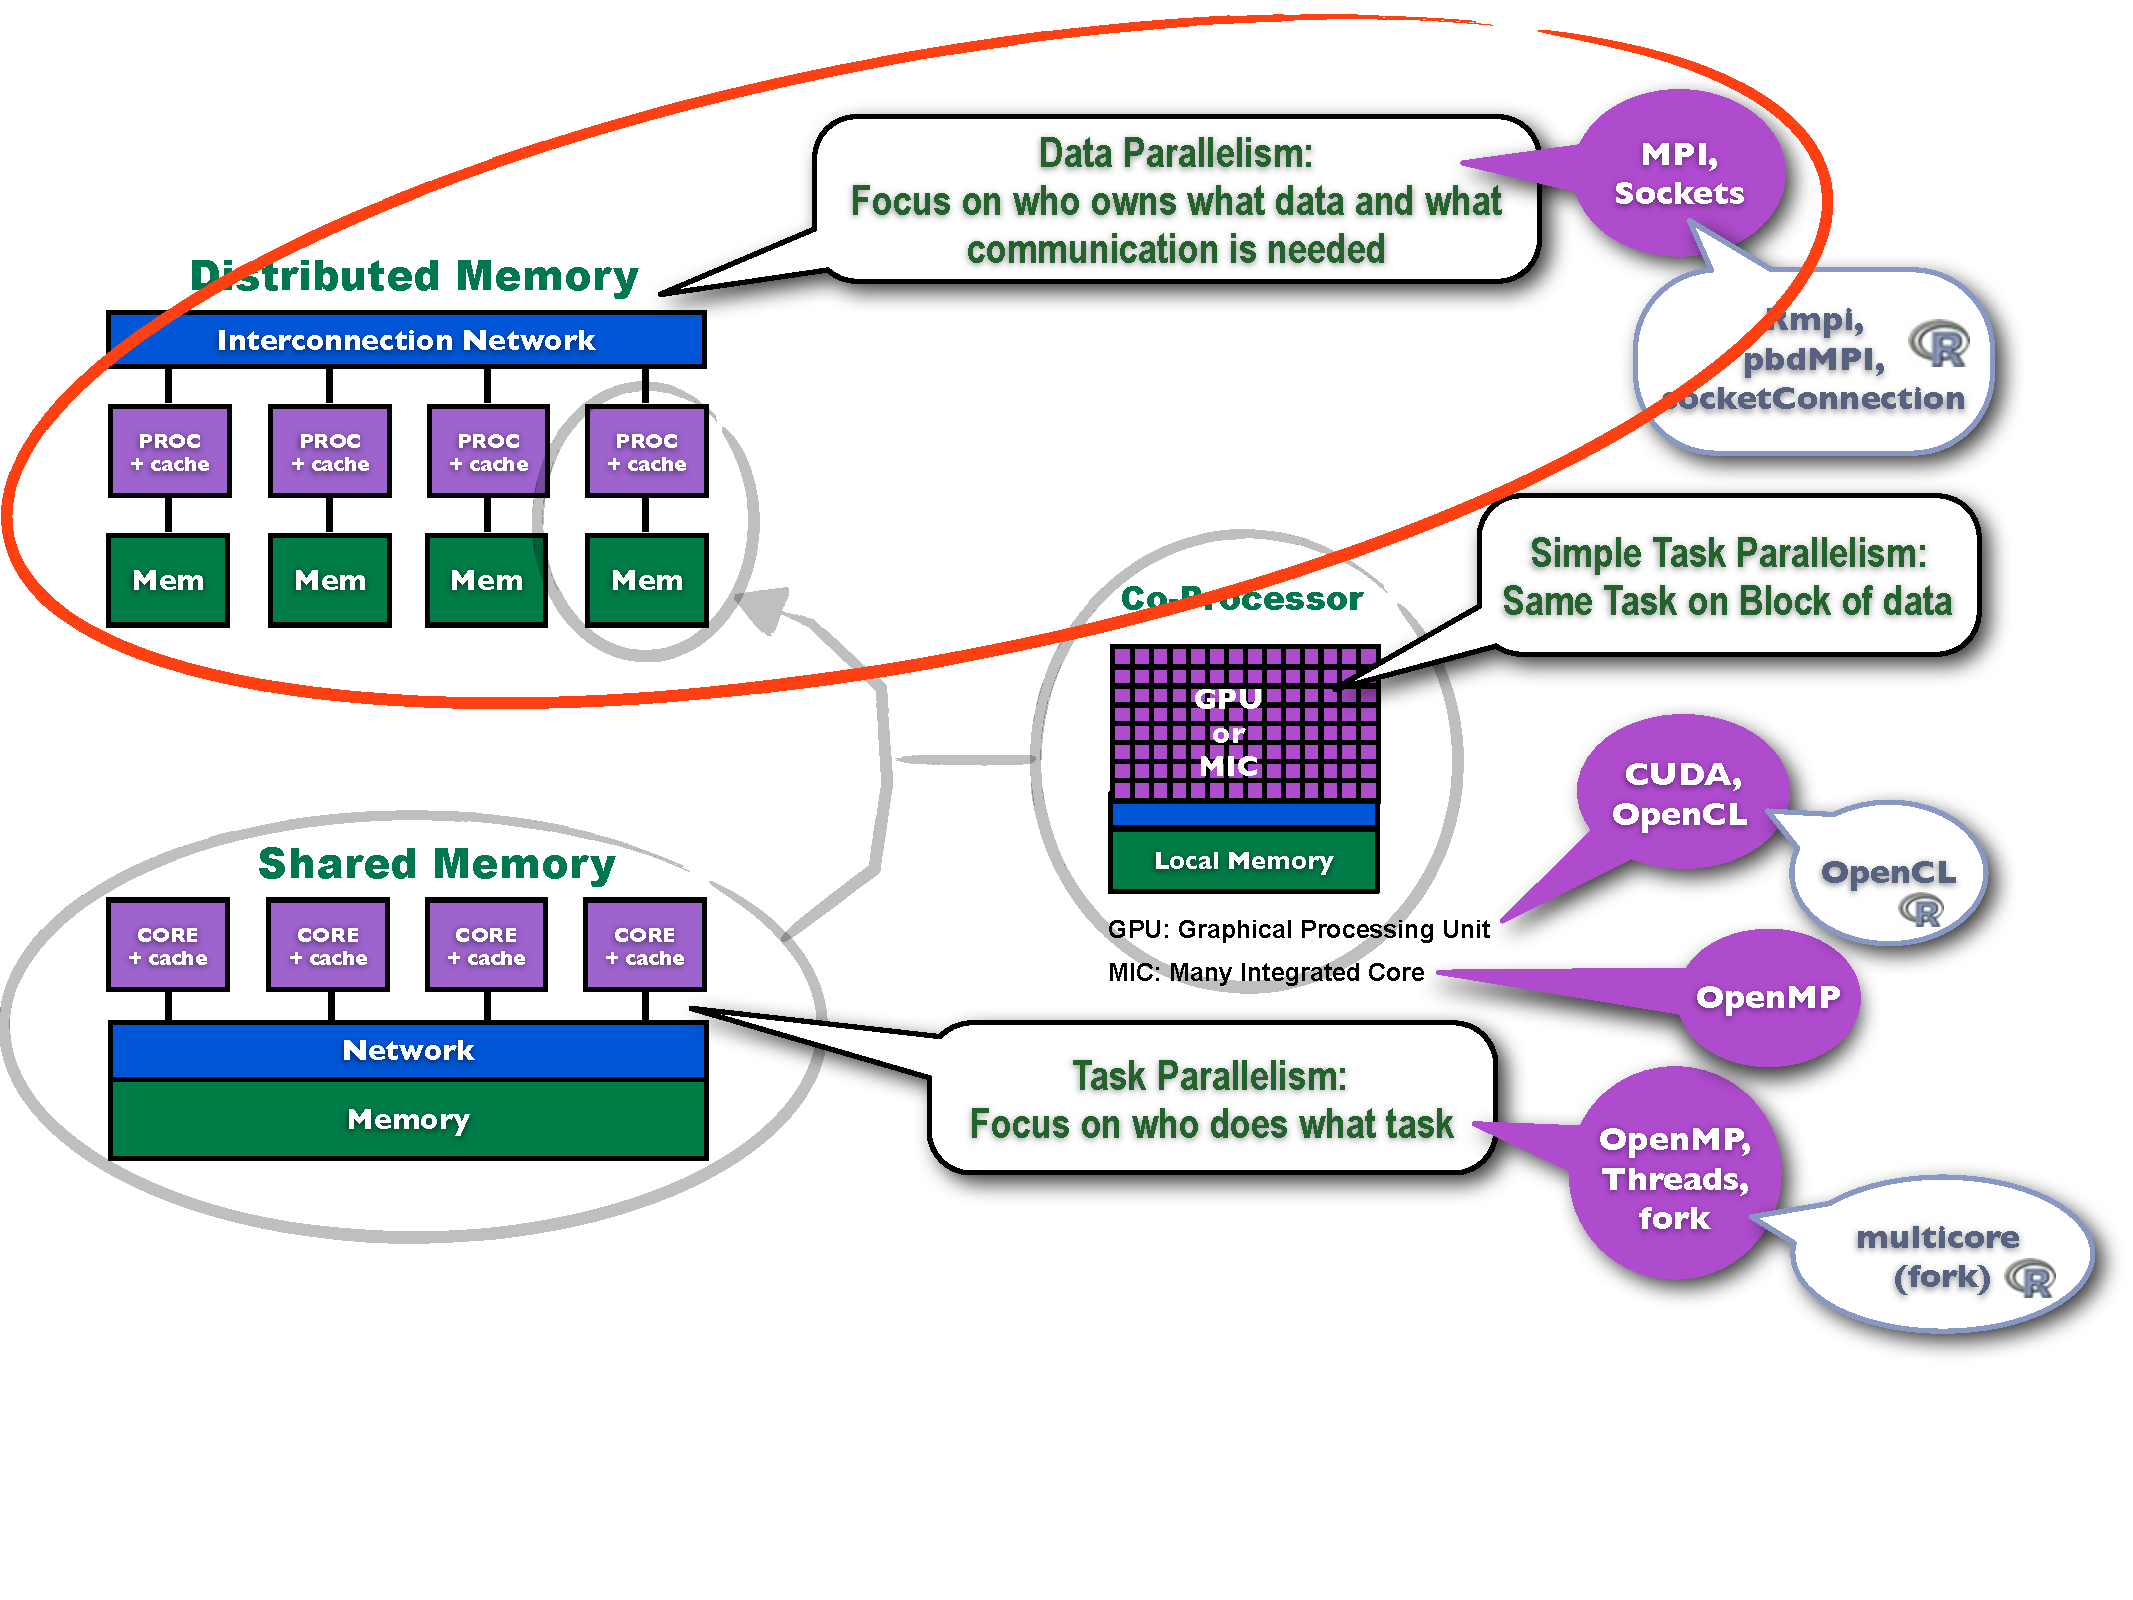
\includegraphics[width=0.95\textwidth]{../common/pics/ParallelHardware8.pdf}
\end{block}
\end{frame}

\begin{frame}
\begin{block}{Last 10 years of Advances}
    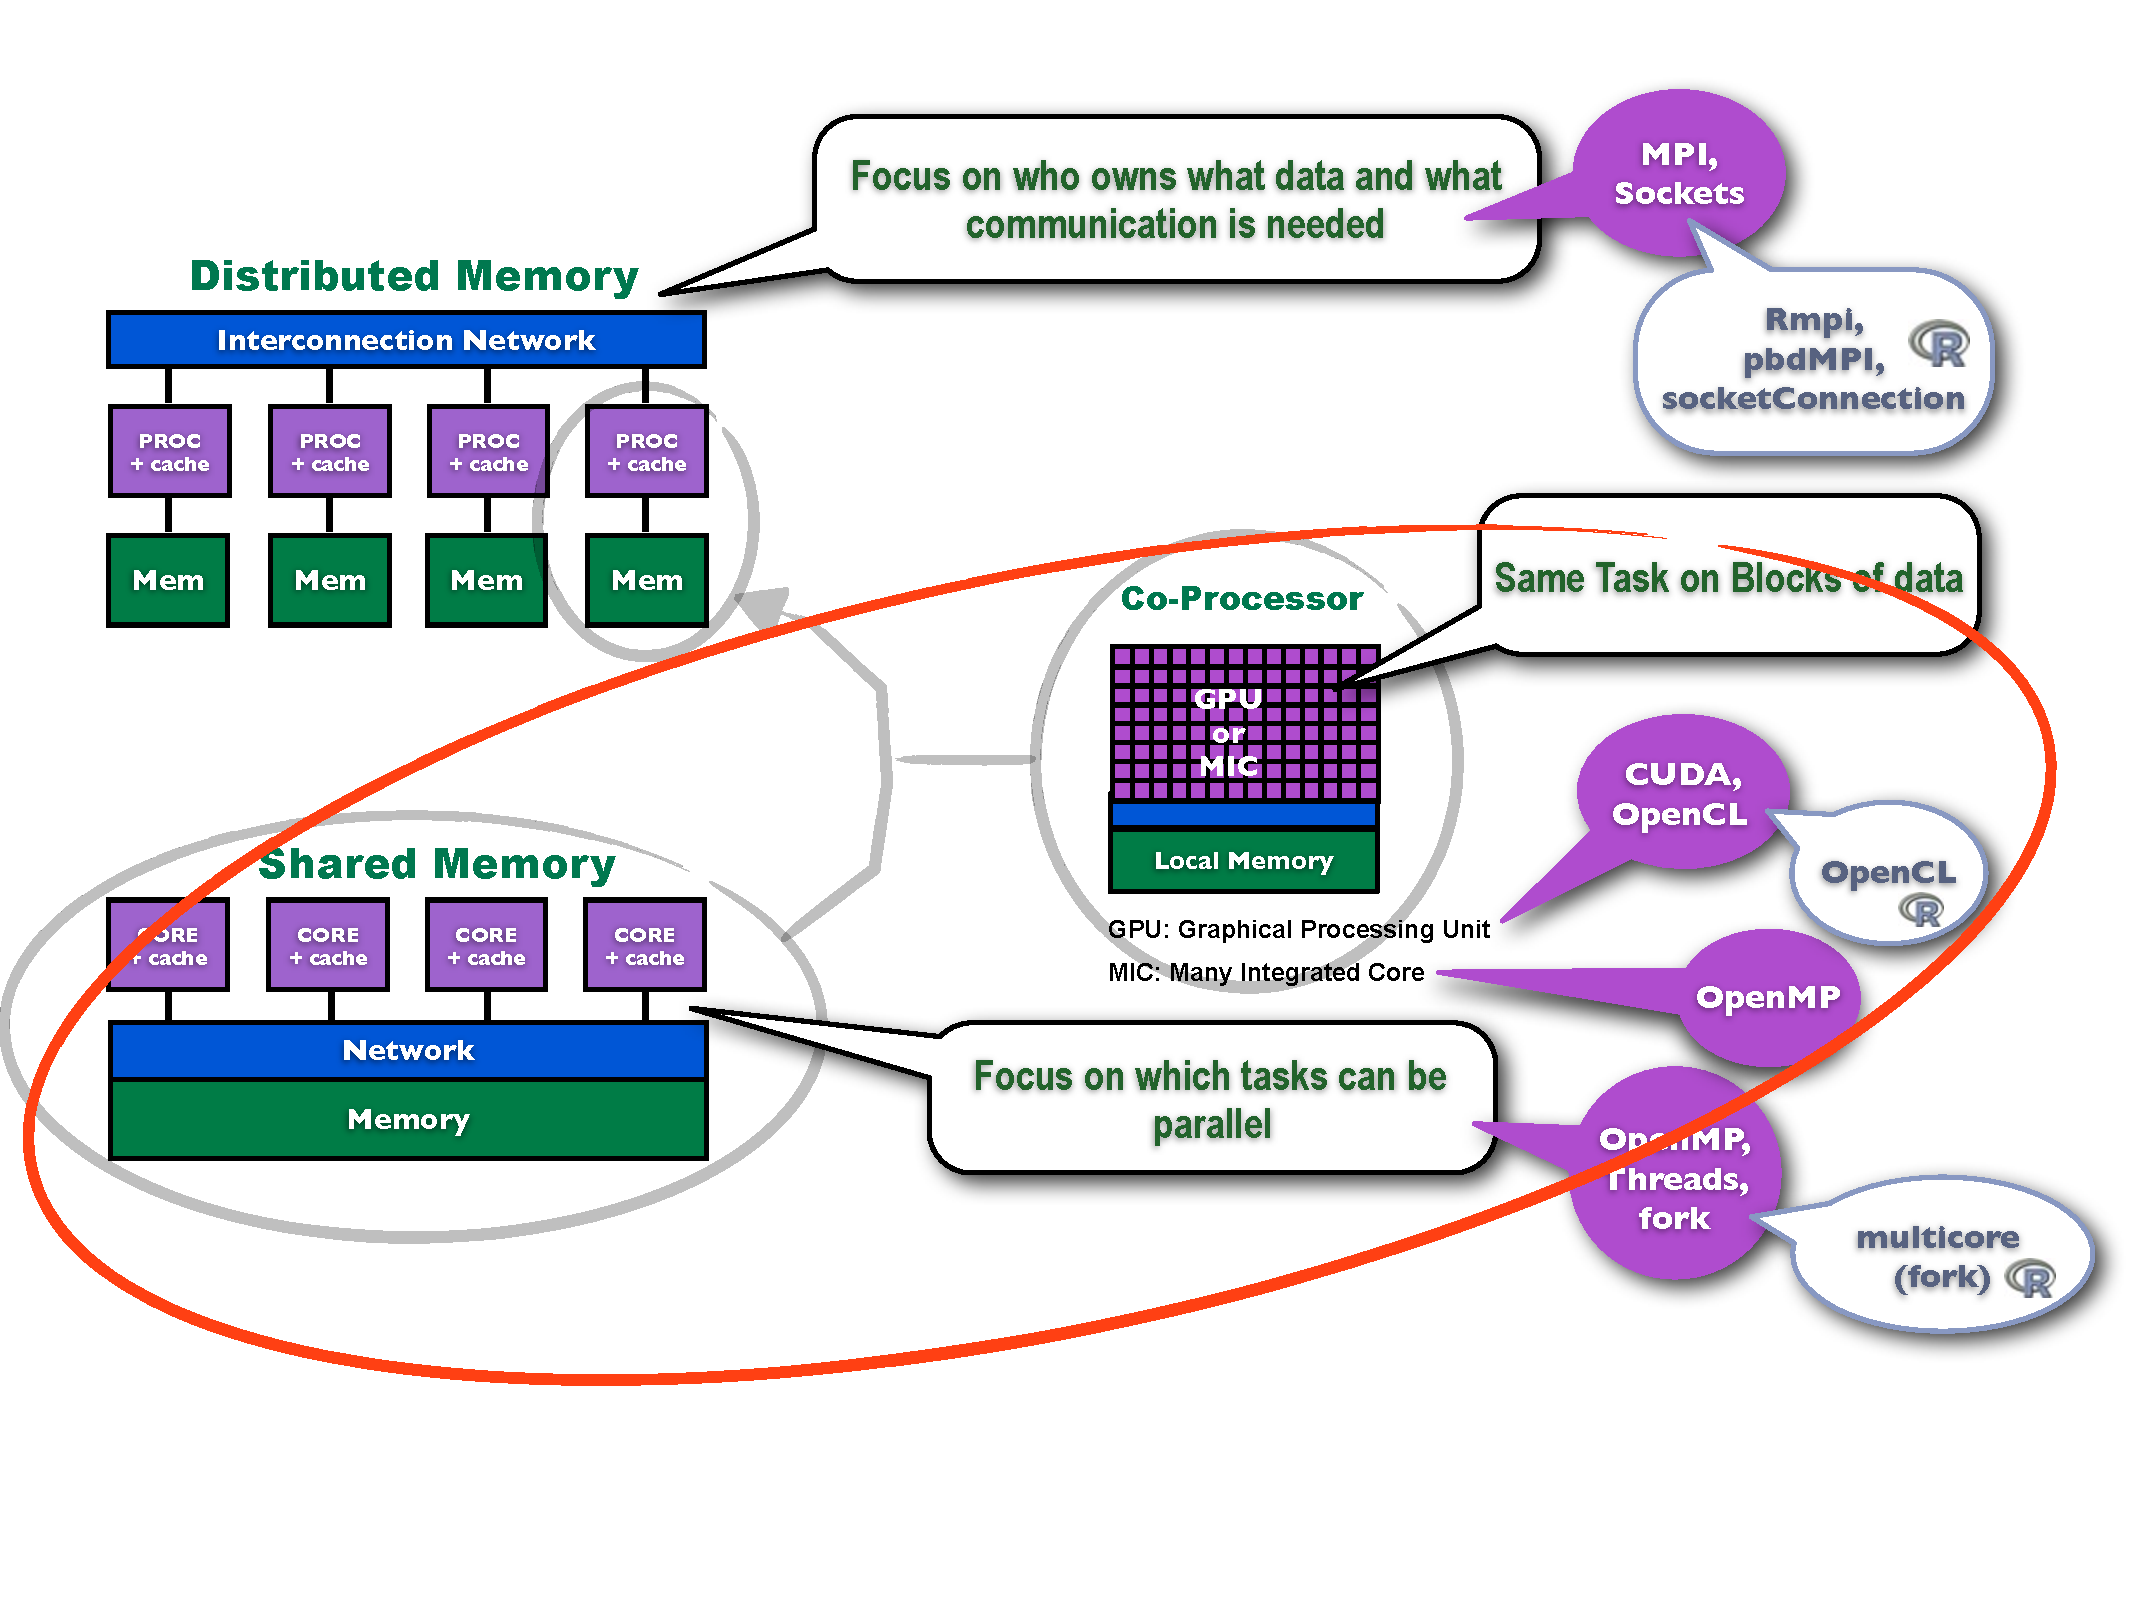
\includegraphics[width=0.95\textwidth]{../common/pics/ParallelHardware9.pdf}
\end{block}
\end{frame}

\begin{frame}
\begin{block}{Putting It All Together Challenge}
    
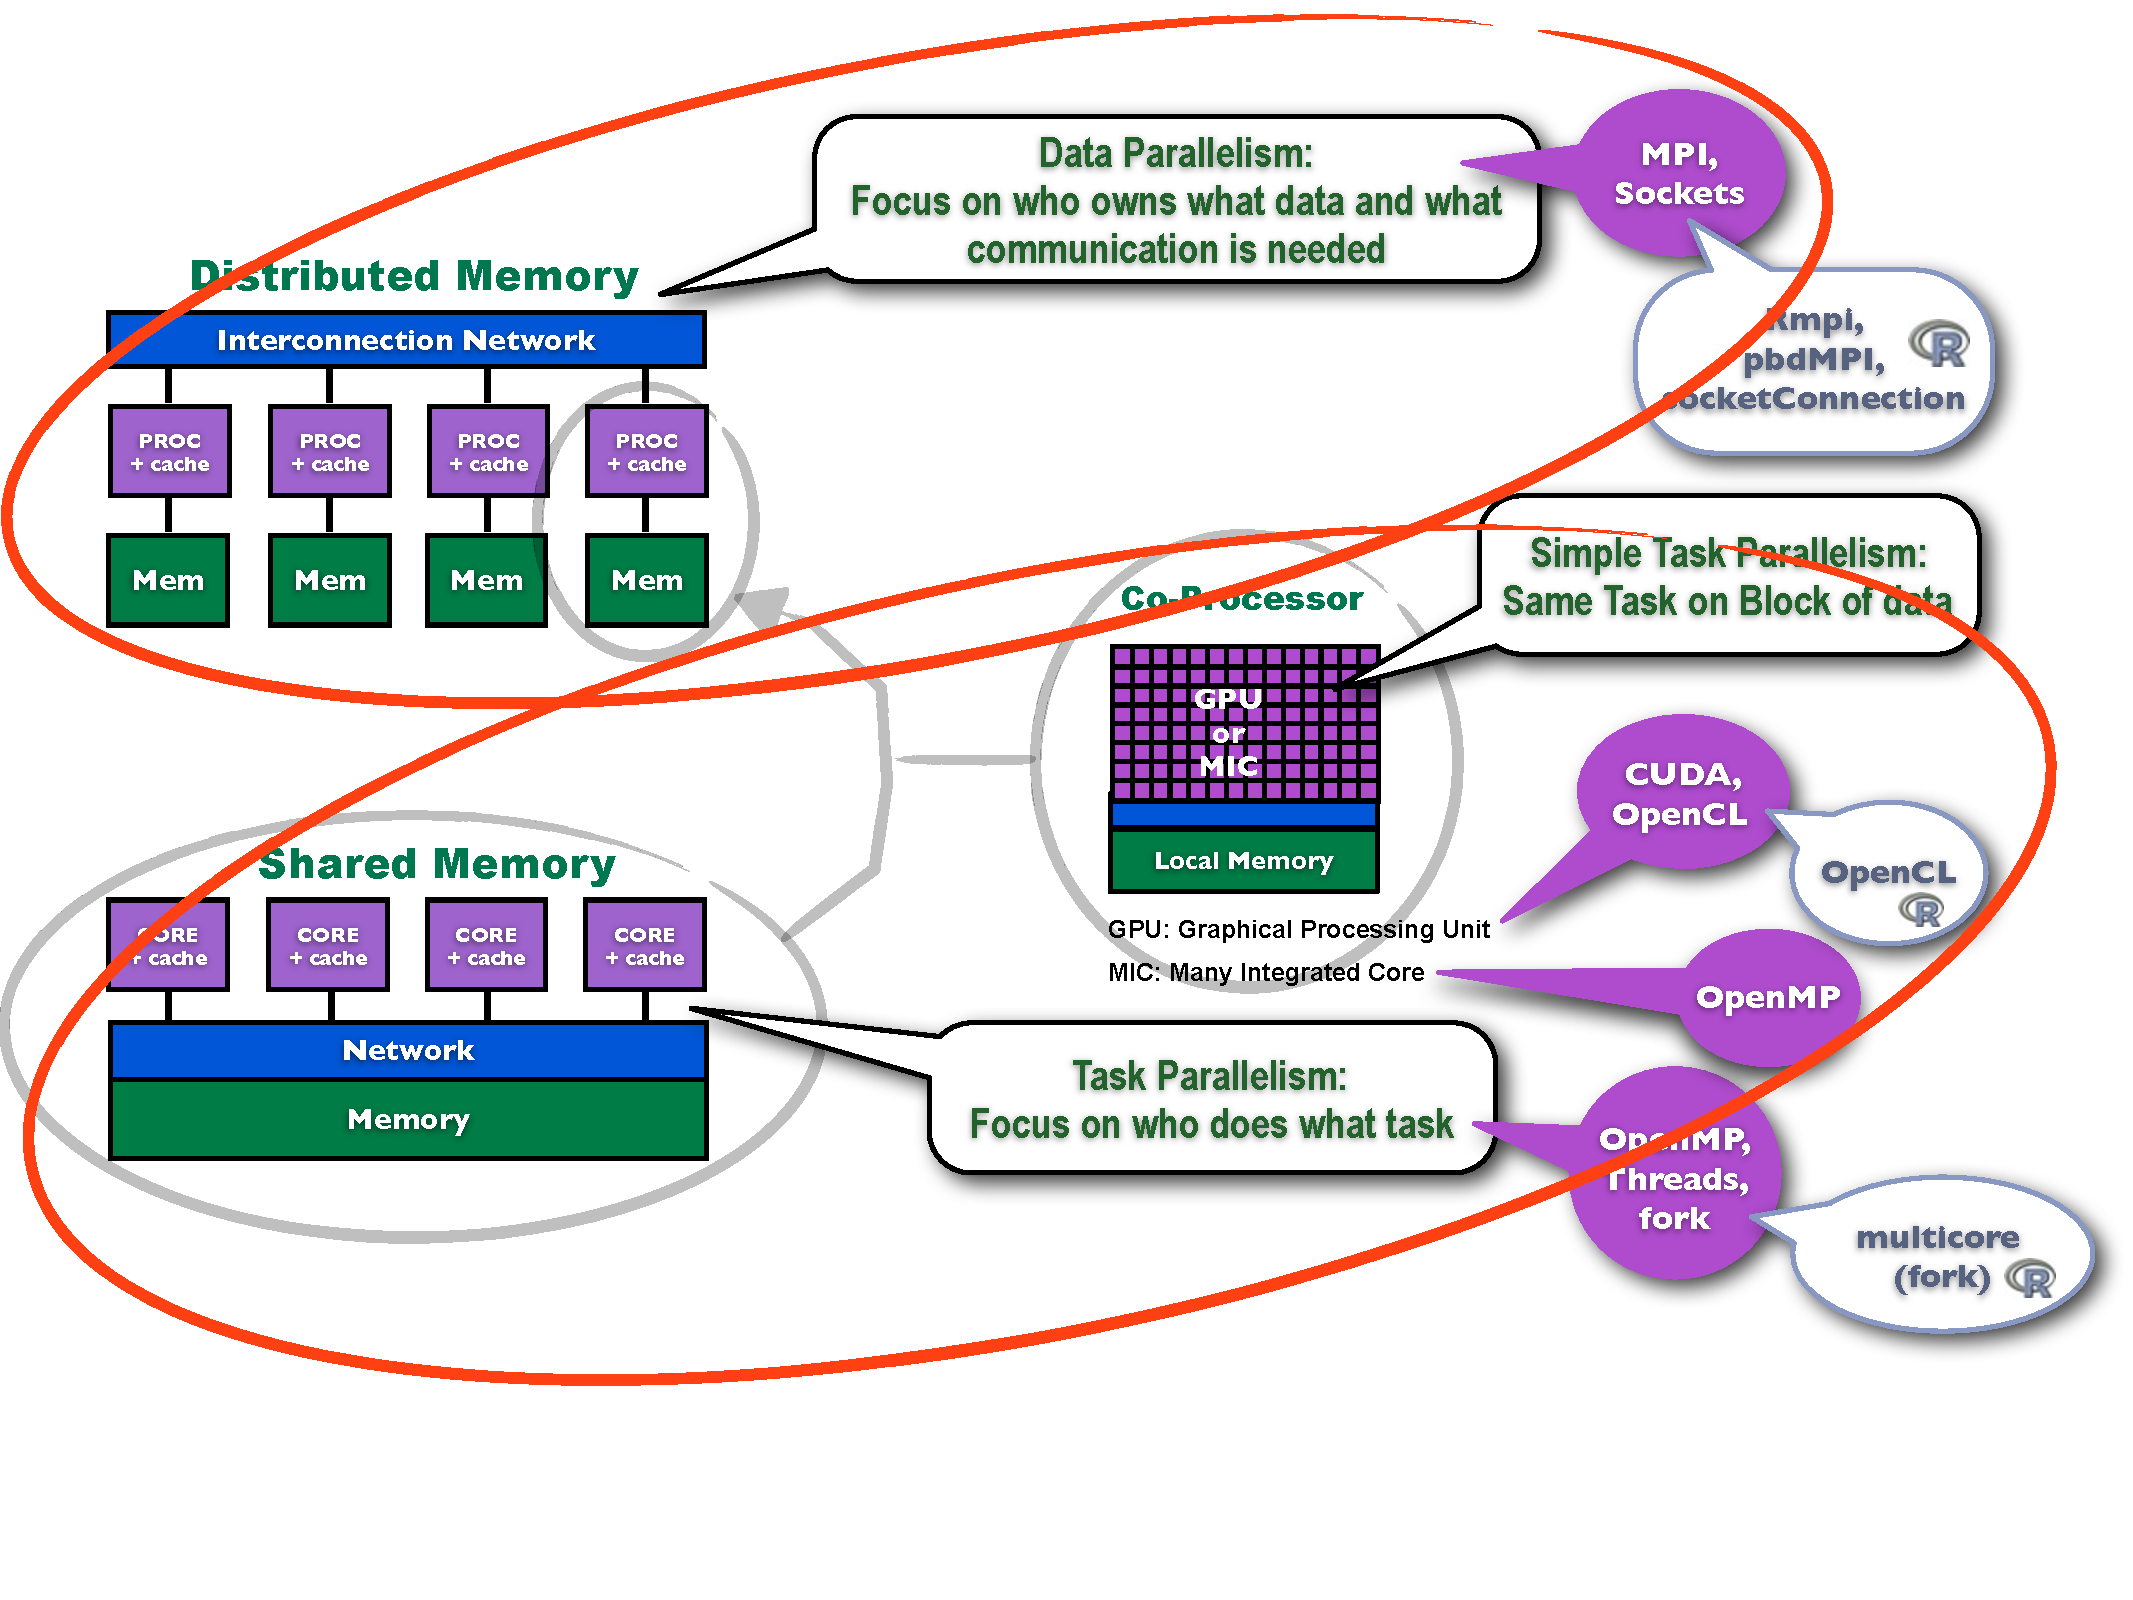
\includegraphics[width=0.95\textwidth]{../common/pics/ParallelHardware10.pdf}
\end{block}
\end{frame}

\begin{frame}
\begin{block}{pbdR Focus on Data Parallelism}
    
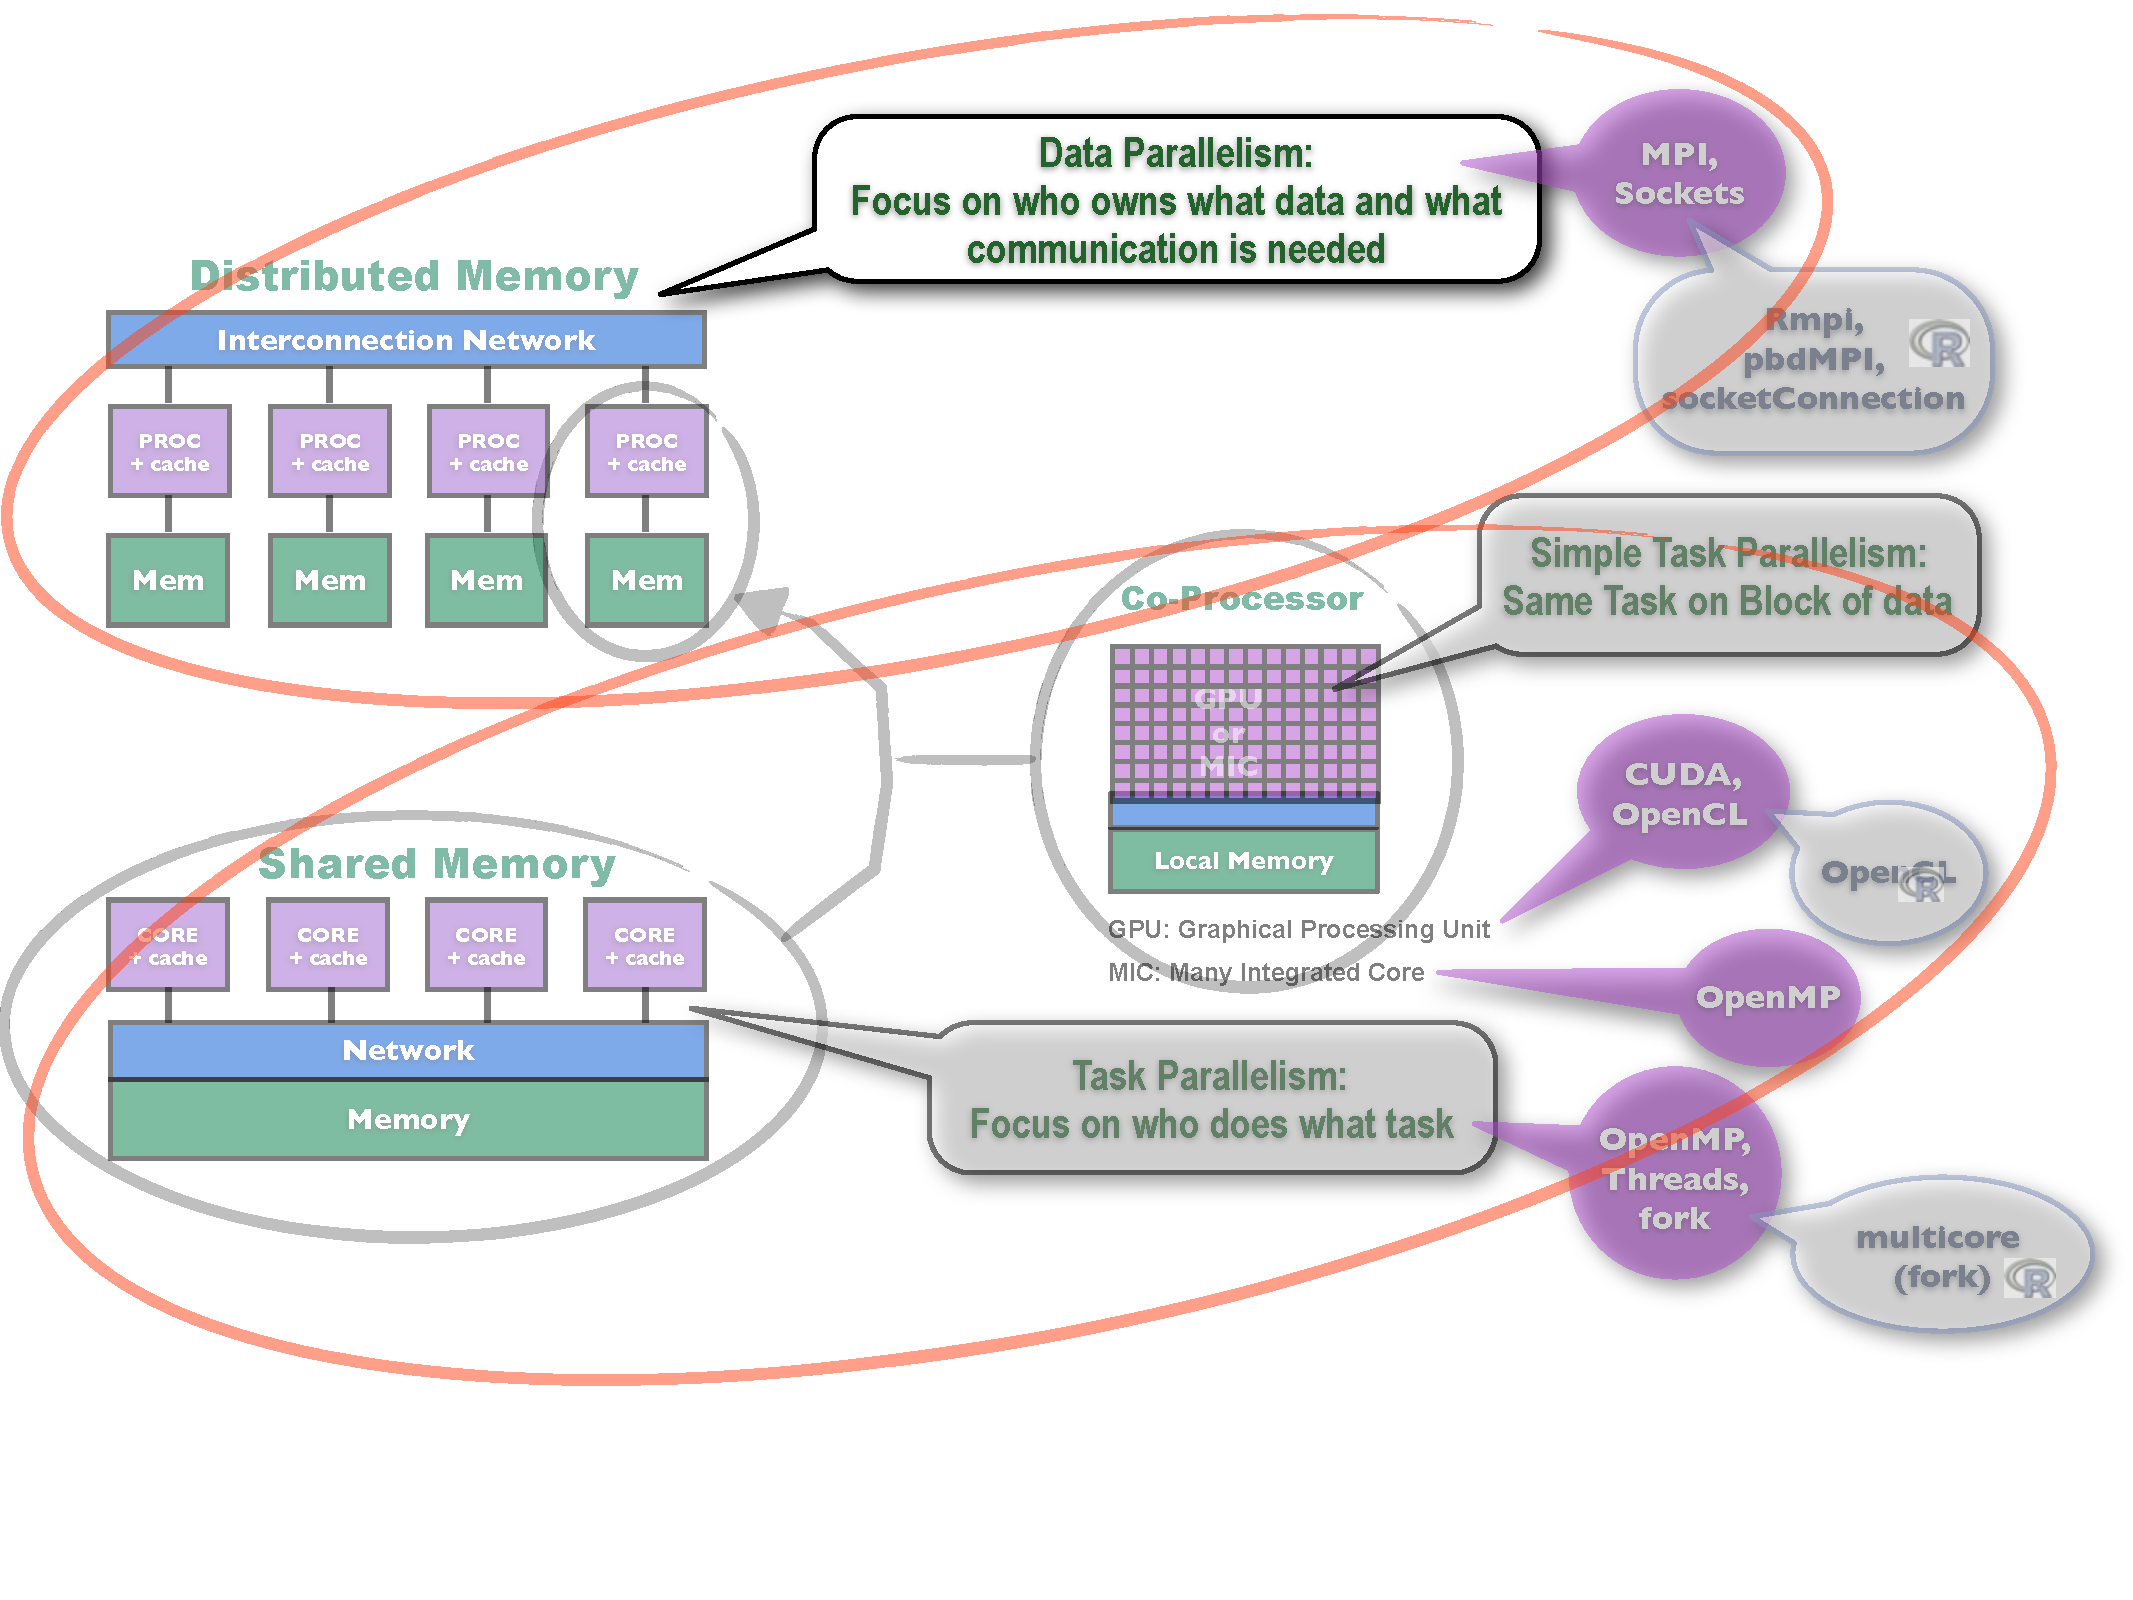
\includegraphics[width=0.95\textwidth]{../common/pics/ParallelHardware11.pdf}
\end{block}
\end{frame}

\section{pbdR}

\hidenum
\begin{frame}[noframenumbering]
\frametitle{Contents}
 \tableofcontents[currentsection,hideothersubsections,sectionstyle=show/hide]
\end{frame}
\shownum


\subsection{The pbdR Project}


\begin{frame}
  \begin{block}{Programming with Big Data in R (pbdR)}
       \centering Striving for \emph{Productivity, Portability, Performance}\\[.4cm]\pause
  \begin{columns}[onlytextwidth]
    \begin{column}{0.30\textwidth}
      \centering
       
\includegraphics[width=3.4cm]{pics/simple}\\[.2cm]
    \end{column}
    \begin{column}{0.65\textwidth}
  \begin{itemize}[<+-|alert@+>]
    \item Series of \emph{free}\footnote{MPL, BSD, and GPL licensed} R packages.
    \item Scalable, big data analytics with high-level syntax.
    \item Implicit management of distributed data details.
    \item Methods have syntax \emph{identical} to R.
    \item Powered by state of the art numerical libraries (MPI, ScaLAPACK, PBLAS, BLACS, LAPACK, BLAS, \dots)
  \end{itemize}
    \end{column}
​  \end{columns}
\end{block}
\end{frame}




\begin{frame}[shrink]
  \begin{block}{pbdR Packages}
    \begin{center}
        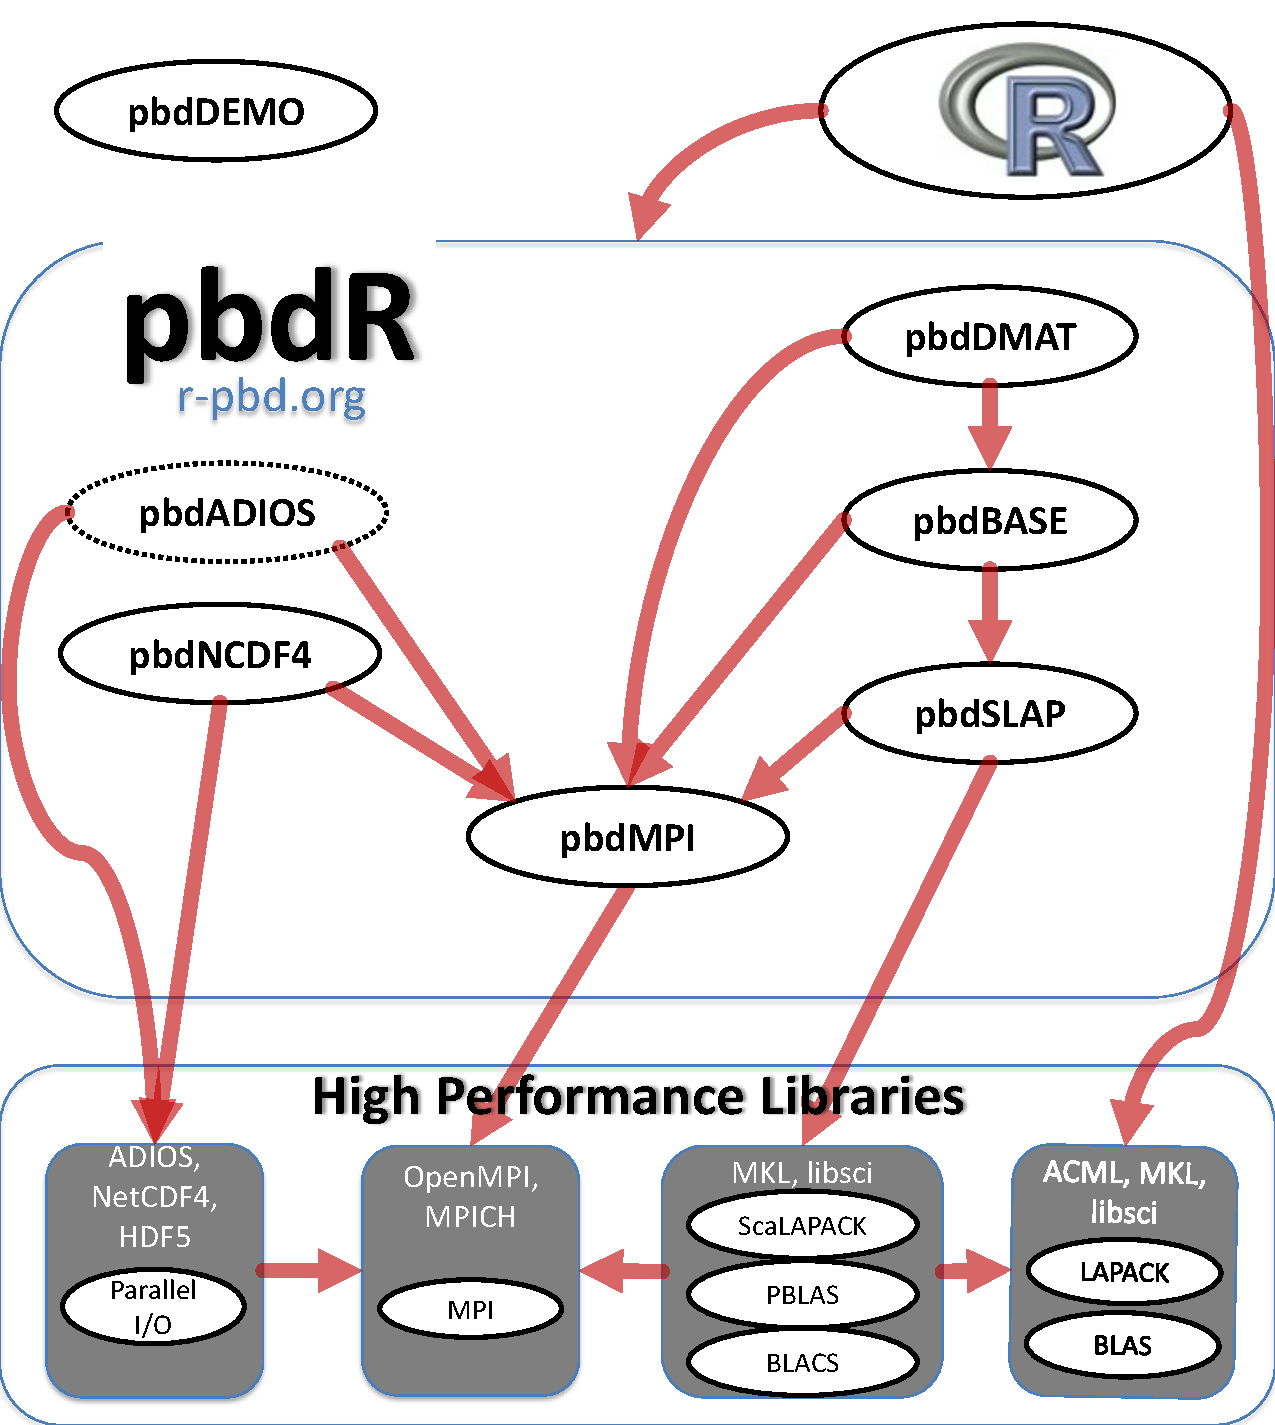
\includegraphics[width=7cm, height=7cm]{pics/pbdpacks}
    \end{center}
  \end{block}
\end{frame}


\begin{frame}[shrink]
  \begin{block}{pbdR Packages --- http://code.r-pbd.org}\pause
  Released to CRAN:
  \begin{itemize}[<+-|alert@+>]
    \item \pkg{pbdMPI}: MPI bindings (explicit, low-level)
    \item \pkg{pbdSLAP}: Foreign library (just install it, nothing to use)
    \item \pkg{pbdBASE}: Compiled code (used by DMAT, also for devs)
    \item \pkg{pbdDMAT}: Distributed matrices (mostly implicit, high-level)
    \item \pkg{pbdNCDF4}: Parallel NetCDF4 reader
    \item \pkg{pbdDEMO}: Package demonstrations, examples, vignette written in textbook style
  \end{itemize}
%     \\[.2cm]
    Future Development:
  \begin{itemize}[<+-|alert@+>]
    \item Profiling tools
    \item Client/server interface for interactive sessions
    \item \dots
  \end{itemize}
  \end{block}
\end{frame}



\begin{frame}[fragile]
  \begin{block}{Example Syntax}\pause
  \begin{lstlisting}
x <- x[-1, 2:5]
x <- log(abs(x) + 1)
xtx <- t(x) %*% x
ans <- svd(solve(xtx))
  \end{lstlisting}
  \begin{center}
  \pause Look familiar?\\[.4cm] \pause
  \emph{The above runs on 1 core with R or 10,000 cores with pbdR}
  \end{center}
  \end{block}
\end{frame}



\subsection{pbdR Paradigms}

%%%%%% FIXME
%% distributed
%% batch
%% spmd
%% OO
%% ...?


\begin{frame}
  \begin{block}{pbdR Focus:  Distributed Machines}
   \begin{center}
    \begin{minipage}[t]{.47\textwidth}
    \begin{block}{\centering Shared Memory Machines}
    \begin{center}
    Thousands of cores\\[.2cm]
    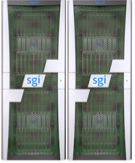
\includegraphics[scale=.65]{pics/nautilus}\\
    {\tiny \emph{Nautilus}, University of Tennessee\\1024 cores}
    \end{center}
    \end{block}
    \end{minipage}
    \hspace{.1cm}
    \begin{minipage}[t]{.47\textwidth}
    \begin{block}{\centering Distributed Memory Machines}
    \begin{center}
    Hundreds of thousands of cores\\[.2cm]
    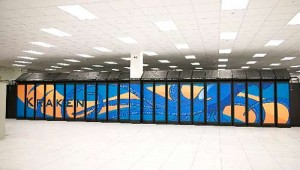
\includegraphics[width=.95\textwidth]{pics/kraken}\\
    {\tiny \emph{Kraken}, University of Tennessee\\ 112,896 cores}
    \end{center}
    \end{block}
    \end{minipage}
    \end{center}
    \end{block}
\end{frame}

\begin{frame}
  \begin{block}{pbdR Paradigms}
  Programs that use pbdR are meant to utilize the:
  \begin{itemize}[<+-|alert@+>]
   \item Data Parallelism method
   \item Single Program/Multiple Data (SPMD) style
  \end{itemize}
  \end{block}
\end{frame}



\begin{frame}
  \begin{block}{SPMD}\pause
  The pbdR Packages enable high-level ``Single Program/Multiple Data'' (SPMD) programming:
    \begin{itemize}
      \item SPMD is a programming \emph{paradigm}.
      \item Arguably the simplest extension of serial programming.
      \item Sort of like trying to explain breathing \dots
      \item Not to be confused with SIMD.
      \item SPMD utilizes MIMD architecture computers.
      \item Only one program is written, executed in batch independently on all processors.
      \item Different processors are autonomous; there is no manager.
%       \item Like ``Map/Reduce'', you probably used it without knowing it even had a name.
    \end{itemize}
  \end{block}
\end{frame}


\begin{frame}[fragile]
  \begin{block}{SPMD}\pause
      SPMD codes are run in batch (non-interactively):
\begin{lstlisting}[backgroundcolor=\color{white},keywordstyle=\color{black},title=From the Shell]
mpirun -np 4 Rscript my_script.R
\end{lstlisting}
  \end{block}
\end{frame}


\begin{frame}
  \begin{block}{pbdR Paradigms:  Data Parallelism}
  With data parallelism:
  \begin{itemize}[<+-|alert@+>]
   \item No one processor/node owns all the data.
   \item Processors own local pieces of a (conceptually) global object
  \end{itemize}
  \end{block}
\end{frame}


\begin{frame}
  \begin{block}{pbdR Paradigms:  SPMD}
  \begin{itemize}[<+-|alert@+>]
   \item Natural extension of writing serial codes.
   \item Different from Manager/Worker.
   \item No one processor is in charge. Each thinks it's the boss (``it's like academia'').
   \item One program written, executed independently by all processors.
   \item Each processor owns a local sub-piece of data from the (conceptual) whole.
  \end{itemize}
  \end{block}
\end{frame}

% 
% \begin{frame}
%   \begin{block}{Manager/Worker vs SPMD}
%    \begin{center}
%    Graphics will go here\\
%     \begin{minipage}[t]{.47\textwidth}
%     \begin{block}{\centering Manager/Worker:  Fascism}
% %image
%     \end{block}
%     \end{minipage}
%     \hspace{.1cm}
%     \begin{minipage}[t]{.47\textwidth}
%     \begin{block}{\centering SPMD: Democracy}
% %image 
%     \end{block}
%     \end{minipage}
%     \end{center}
%     \end{block}
% \end{frame}
\section[pbdMPI]{Introduction to pbdMPI}

\hidenum
\begin{frame}[noframenumbering]
\frametitle{Contents}
 \tableofcontents[currentsection,hideothersubsections,sectionstyle=show/hide]
\end{frame}
\shownum

\subsection{Managing a Communicator}

\begin{frame}
  \begin{block}{Message Passing Interface (MPI)}\pause
    \begin{itemize}
      \item \textit{MPI}: Standard for managing communications (data and instructions) between different nodes/computers.
      \item \textit{Implementations}:  OpenMPI, MPICH2, Cray MPT, \dots
      \item Enables parallelism (via communication) on distributed machines.
      \item \textit{Communicator}: manages communications between processors.
    \end{itemize}
  \end{block}
\end{frame}


\begin{frame}
  \begin{block}{MPI Operations (1 of 2)}\pause
    \begin{itemize}
      \item \textbf{Managing a Communicator}:  Create and destroy communicators.\\
      \code{init()} --- initialize communicator\\
      \code{finalize()} --- shut down communicator(s)
      \\[.4cm]
      %
      \item \textbf{Rank query}: determine the processor's position in the communicator.\\
      \code{comm.rank()} --- ``who am I?''\\
      \code{comm.size()} --- ``how many of us are there?''\\[.4cm]
      \item \textbf{Printing}:  Printing output from various ranks.\\
      \code{comm.print(x)}\\
      \code{comm.cat(x)}\\
      \textbf{WARNING}: only use these functions on \emph{results}, never on yet-to-be-computed things.\\
    \end{itemize}
  \end{block}
\end{frame}


\begin{frame}[fragile]
  \begin{exampleblock}{Quick Example 1}
  \centering
\begin{lstlisting}[title=Rank Query: 1\_rank.r]
library(pbdMPI, quiet = TRUE)
init()

my.rank <- comm.rank()
comm.print(my.rank, all.rank=TRUE)

finalize()
\end{lstlisting}
  \begin{columns}[t,onlytextwidth]
    \begin{column}{0.62\textwidth}
\begin{lstlisting}[backgroundcolor=\color{white},keywordstyle=\color{black},title=Execute this script via:]
mpirun -np 2 Rscript 1_rank.r
\end{lstlisting}    
    \end{column}
    \hfill
    \begin{column}{0.35\textwidth}
\begin{lstlisting}[title=Sample Output:]
COMM.RANK = 0
[1] 0
COMM.RANK = 1
[1] 1
\end{lstlisting}
    \end{column}
​  \end{columns}
  \end{exampleblock}
\end{frame}



\begin{frame}[fragile]
  \begin{exampleblock}{Quick Example 2}
\begin{lstlisting}[title=Hello World: 2\_hello.r]
library(pbdMPI, quiet=TRUE)
init()

comm.print("Hello, world")

comm.print("Hello again", all.rank=TRUE, quiet=TRUE)

finalize()
\end{lstlisting}
  \begin{columns}[t,onlytextwidth]
    \begin{column}{0.58\textwidth}
\begin{lstlisting}[backgroundcolor=\color{white},keywordstyle=\color{black},title=Execute this script via:]
mpirun -np 2 Rscript 2_hello.r
\end{lstlisting}    
    \end{column}
    \hfill
    \begin{column}{0.4\textwidth}
\begin{lstlisting}[title=Sample Output:]
COMM.RANK = 0
[1] "Hello, world"
[1] "Hello again"
[1] "Hello again"
\end{lstlisting}
    \end{column}
​  \end{columns}
  \end{exampleblock}
\end{frame}



\subsection{Reduce, Gather, Broadcast, and Barrier}


\begin{frame}
  \begin{block}{MPI Operations}
    \begin{enumerate}
      \item Reduce
      \item Gather
      \item Broadcast
      \item Barrier
    \end{enumerate}
  \end{block}
\end{frame}

\begin{frame}
  \begin{block}{Reductions --- Combine results into single result}
    \begin{center}
      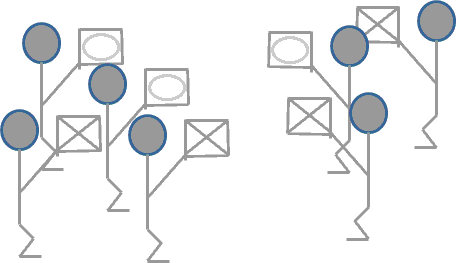
\includegraphics[scale=.6]{pics/mpi_reduce}
    \end{center}
  \end{block}
\end{frame}


\begin{frame}
  \begin{block}{Gather --- Many-to-one}
    \begin{center}
      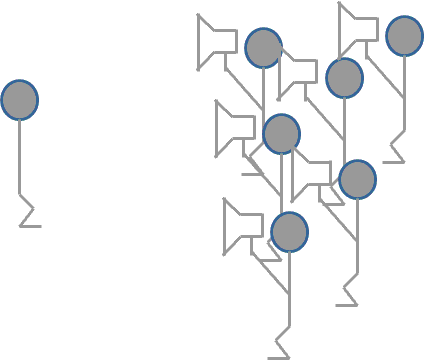
\includegraphics[scale=.6]{pics/mpi_gather}
    \end{center}
  \end{block}
\end{frame}


\begin{frame}
  \begin{block}{Broadcast --- One-to-many}
    \begin{center}
      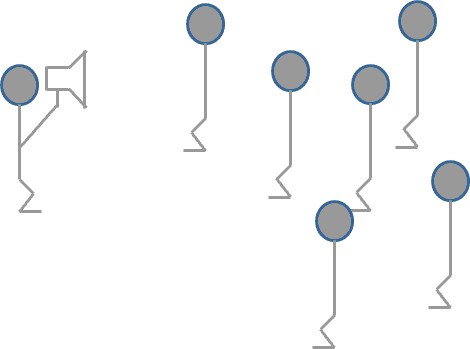
\includegraphics[scale=.6]{pics/mpi_bcast}
    \end{center}
  \end{block}
\end{frame}


\begin{frame}
  \begin{block}{Barrier --- Synchronization}
    \begin{center}
      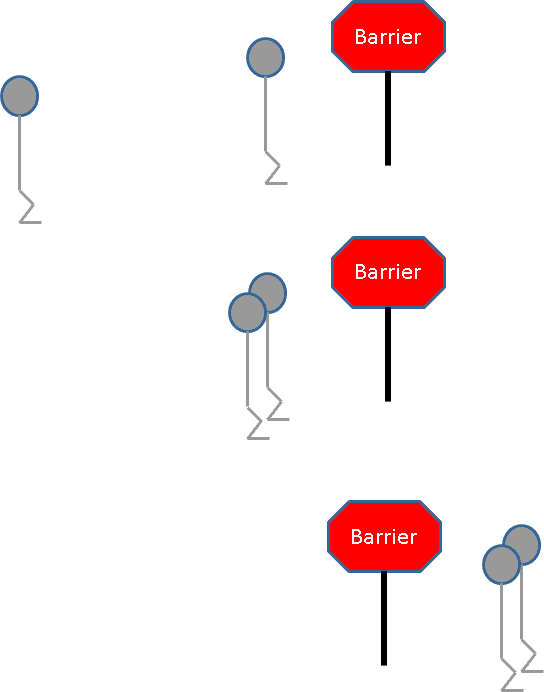
\includegraphics[scale=.38]{pics/mpi_barrier}
    \end{center}
  \end{block}
\end{frame}



\begin{frame}[shrink]
  \begin{block}{MPI Operations (2 of 2)}\pause
    \begin{itemize}
      \item \textbf{Reduction}:  each processor has a number \code{x}; add all of them up, find the largest/smallest, \dots .\\
      \code{reduce(x, op='sum')} --- reduce to one\\
      \code{allreduce(x, op='sum')} --- reduce to all\\[.4cm]
      %
      \item \textbf{Gather}: each processor has a number; create a new object on some processor containing all of those numbers.\\
      \code{gather(x)} --- gather to one\\
      \code{allgather(x)} --- gather to all\\[.4cm]
      %
      \item \textbf{Broadcast}: one processor has a number \code{x} that every other processor should also have.\\
      \code{bcast(x)}
      \\[.4cm]
      \item \textbf{Barrier}: ``computation wall''; no processor can proceed until \emph{all} processors can proceed.\\
\code{barrier()}
    \end{itemize}
  \end{block}
\end{frame}




\begin{frame}[fragile,shrink]
  \begin{exampleblock}{Quick Example 3}
\begin{lstlisting}[title=Reduce and Gather: 3\_gt.r]
library(pbdMPI, quiet = TRUE)
init()

comm.set.seed(diff=TRUE)

n <- sample(1:10, size=1)

gt <- gather(n)
comm.print(unlist(gt))

sm <- allreduce(n, op='sum')
comm.print(sm, all.rank=T)

finalize()
\end{lstlisting}
  \begin{columns}[t,onlytextwidth]
    \begin{column}{0.58\textwidth}
\begin{lstlisting}[backgroundcolor=\color{white},keywordstyle=\color{black},title=Execute this script via:]
mpirun -np 2 Rscript 3_gt.r
\end{lstlisting}    
    \end{column}
    \hfill
    \begin{column}{0.4\textwidth}
\begin{lstlisting}[title=Sample Output:]
COMM.RANK = 0
[1] 2 8
COMM.RANK = 0
[1] 10
COMM.RANK = 1
[1] 10
\end{lstlisting}
    \end{column}
​  \end{columns}
  \end{exampleblock}
\end{frame}


\begin{frame}[fragile,shrink]
  \begin{exampleblock}{Quick Example 4}
\begin{lstlisting}[title=Broadcast: 4\_bcast.r]
library(pbdMPI, quiet=T)
init()

if (comm.rank()==0){
  x <- matrix(1:4, nrow=2)
} else {
  x <- NULL
}

y <- bcast(x, rank.source=0)

comm.print(y, rank=1)

finalize()
\end{lstlisting}
  \begin{columns}[t,onlytextwidth]
    \begin{column}{0.58\textwidth}
\begin{lstlisting}[backgroundcolor=\color{white},keywordstyle=\color{black},title=Execute this script via:]
mpirun -np 2 Rscript 4_bcast.r
\end{lstlisting}
\end{column}
    \hfill
    \begin{column}{0.4\textwidth}
\begin{lstlisting}[title=Sample Output:]
COMM.RANK = 1
     [,1] [,2]
[1,]    1    3
[2,]    2    4
\end{lstlisting}
    \end{column}
​  \end{columns}
  \end{exampleblock}
\end{frame}







\subsection{Other pbdMPI Tools}


\begin{frame}
  \begin{block}{MPI Package Controls}
The \code{.SPMD.CT} object allows for setting different package options with \pkg{pbdMPI}.  See the entry \emph{SPMD Control} of the \pkg{pbdMPI} manual for information about the \code{.SPMD.CT} object:
\begin{center}
{ \small
\url{http://cran.r-project.org/web/packages/pbdMPI/pbdMPI.pdf}
}
\end{center}
  \end{block}
\end{frame}

\begin{frame}[fragile,shrink]
  \begin{exampleblock}{Quick Example 5}
\begin{lstlisting}[title=Barrier: 5\_barrier.r]
library(pbdMPI, quiet = TRUE)
init()

.SPMD.CT$msg.barrier <- TRUE
.SPMD.CT$print.quiet <- TRUE

for (rank in 1:comm.size()-1){
  if (comm.rank() == rank){
    cat(paste("Hello", rank+1, "of", comm.size(), "\n"))
  }
  barrier()
}

comm.cat("\n")

comm.cat(paste("Hello", comm.rank()+1, "of", comm.size(), "\n"), all.rank=TRUE)

finalize()
\end{lstlisting}
  \begin{columns}[t,onlytextwidth]
    \begin{column}{0.58\textwidth}
\begin{lstlisting}[backgroundcolor=\color{white},keywordstyle=\color{black},title=Execute this script via:]
mpirun -np 2 Rscript 5_barrier.r
\end{lstlisting}
    \end{column}
    \hfill
    \begin{column}{0.4\textwidth}
\begin{lstlisting}[title=Sample Output:]
Hello 1 of 2 
Hello 2 of 2 
\end{lstlisting}
    \end{column}
​  \end{columns}
  \end{exampleblock}
\end{frame}


\begin{frame}
  \begin{block}{Random Seeds}\pause
  \pkg{pbdMPI} offers a simple interface for managing random seeds:
    \begin{itemize}
      \item \code{comm.set.seed(diff=TRUE)} --- Independent streams via the \pkg{rlecuyer} package.
      \item \code{comm.set.seed(seed=1234, diff=FALSE)} --- All processors use the same seed \code{seed=1234}
      \item \code{comm.set.seed(diff=FALSE)} --- All processors use the same seed, determined by processor 0 (using the system clock and PID of processor 0).
    \end{itemize}
  \end{block}
\end{frame}



\begin{frame}[fragile,shrink]
  \begin{exampleblock}{Quick Example 6}
\begin{lstlisting}[title=Timing: 6\_timer.r]
library(pbdMPI, quiet=TRUE)
init()

comm.set.seed(diff=T)

test <- function(timed)
{
  ltime <- system.time(timed)[3]
  
  mintime <- allreduce(ltime, op='min')
  maxtime <- allreduce(ltime, op='max')
  meantime <- allreduce(ltime, op='sum')/comm.size()

  return(data.frame(min=mintime, mean=meantime, max=maxtime))
}

times <- test(rnorm(1e6)) # ~7.6MiB of data
comm.print(times)

finalize()
\end{lstlisting}
  \begin{columns}[t,onlytextwidth]
    \begin{column}{0.58\textwidth}
\begin{lstlisting}[backgroundcolor=\color{white},keywordstyle=\color{black},title=Execute this script via:]
mpirun -np 2 Rscript 6_timer.r
\end{lstlisting}
\end{column}
    \hfill
    \begin{column}{0.35\textwidth}
\begin{lstlisting}[title=Sample Output:]
   min  mean   max
1 0.17 0.173 0.176
\end{lstlisting}
\end{column}
\end{columns}
  \end{exampleblock}
\end{frame}



\begin{frame}
  \begin{block}{Other Helper Tools}\pause
  \pkg{pbdMPI} Also contains useful tools for Manager/Worker and task parallelism codes:
    \begin{itemize}
      \item \textbf{Task Subsetting}: Distributing a list of jobs/tasks\\ 
      \code{get.jid(n)}
      %
      \item \textbf{*ply}:  Functions in the *ply family.\\
      \code{pbdApply(X, MARGIN, FUN, \dots)} --- analogue of \code{apply()}\\
      \code{pbdLapply(X, FUN, \dots)} --- analogue of \code{lapply()}\\
      \code{pbdSapply(X, FUN, \dots)} --- analogue of \code{sapply()}\\
    \end{itemize}
  \end{block}
\end{frame}






\begin{frame}[fragile]
  \begin{block}{Quick Comments for Using pbdMPI}\pause
    \begin{enumerate}
      \item Start by loading the package:
\vspace{-.4cm}
\begin{lstlisting}
library(pbdMPI, quiet = TRUE)
\end{lstlisting}
      \item Always initialize before starting and finalize when finished:
\vspace{-.4cm}
\begin{lstlisting}
init()

# ...

finalize()
\end{lstlisting}
\end{enumerate}
\end{block}
\end{frame}
\begin{frame}
\frametitle{Basic MPI Exercises}
\begin{enumerate}
  \item Experiment with Quick Examples 1 through 6, running them on 2, 4, and 8 processors.
\end{enumerate}
\end{frame}

\section[GBD]{The Generalized Block Distribution}

\hidenum
\begin{frame}[noframenumbering]
\frametitle{Contents}
 \tableofcontents[currentsection,hideothersubsections,sectionstyle=show/hide]
\end{frame}
\shownum


\subsection{The GBD Data Structure}


\begin{frame}
  \begin{block}{Distributing Data}
  \centering
\textbf{Problem:}  How to distribute the data
\begin{center}
    \begin{minipage}{0.47\textwidth}
     \begin{center}
      \begin{align*}
      x &= \left[
            \begin{array}{lll}
            x_{1,1} & x_{1,2} & x_{1,3} \\
            x_{2,1} & x_{2,2} & x_{2,3} \\
            x_{3,1} & x_{3,2} & x_{3,3} \\
            x_{4,1} & x_{4,2} & x_{4,3} \\
            x_{5,1} & x_{5,2} & x_{5,3} \\
            x_{6,1} & x_{6,2} & x_{6,3} \\
            x_{7,1} & x_{7,2} & x_{7,3} \\
            x_{8,1} & x_{8,2} & x_{8,3} \\
            x_{9,1} & x_{9,2} & x_{9,3} \\
            x_{10,1} & x_{10,2} & x_{10,3} \\
            \end{array}
      \right]_{10\times 3}
      \end{align*}
     \end{center}
    \end{minipage}
    \begin{minipage}{0.47\textwidth}
    \centering
      {\fontsize{12cm}{1cm}\selectfont ? }
    \end{minipage}
    \end{center}
  \end{block}
\end{frame}



\begin{frame}
\begin{exampleblock}{Distributing a Matrix Across 4 Processors: Block Distribution}
  \begin{columns}[t,onlytextwidth]
    \begin{column}{0.5\textwidth}
      \hfill Data \hfill\ 
      \begin{align*}
      x &= \left[
            \begin{array}{lll}
            \color{g11}x_{1,1} & \color{g11}x_{1,2} & \color{g11}x_{1,3} \\
            \color{g11}x_{2,1} & \color{g11}x_{2,2} & \color{g11}x_{2,3} \\
            \color{g11}x_{3,1} & \color{g11}x_{3,2} & \color{g11}x_{3,3} \\\hline
            \color{g12}x_{4,1} & \color{g12}x_{4,2} & \color{g12}x_{4,3} \\
            \color{g12}x_{5,1} & \color{g12}x_{5,2} & \color{g12}x_{5,3} \\
            \color{g12}x_{6,1} & \color{g12}x_{6,2} & \color{g12}x_{6,3} \\\hline
            \color{g13}x_{7,1} & \color{g13}x_{7,2} & \color{g13}x_{7,3} \\
            \color{g13}x_{8,1} & \color{g13}x_{8,2} & \color{g13}x_{8,3} \\
            \color{g13}x_{9,1} & \color{g13}x_{9,2} & \color{g13}x_{9,3} \\\hline
            \color{g21}x_{10,1} & \color{g21}x_{10,2} & \color{g21}x_{10,3} \\
            \end{array}
      \right]_{10\times 3}
      \end{align*}
    \end{column}
    \begin{column}{0.5\textwidth}
    \hfill Processors \hfill\ 
      \begin{align*}
      \begin{tabular}{l}
        \color{g11}0 \\
        \color{g12}1 \\
        \color{g13}2 \\
        \color{g21}3 
      \end{tabular}
      \end{align*}
    \end{column}
  \end{columns}
\end{exampleblock}
\end{frame}


\begin{frame}
\begin{exampleblock}{Distributing a Matrix Across 4 Processors: Local Load Balance}
  \begin{columns}[t,onlytextwidth]
    \begin{column}{0.5\textwidth}
      \hfill Data \hfill\ 
      \begin{align*}
      x &= \left[
            \begin{array}{lll}
            \color{g11}x_{1,1} & \color{g11}x_{1,2} & \color{g11}x_{1,3} \\
            \color{g11}x_{2,1} & \color{g11}x_{2,2} & \color{g11}x_{2,3} \\
            \color{g11}x_{3,1} & \color{g11}x_{3,2} & \color{g11}x_{3,3} \\\hline
            \color{g12}x_{4,1} & \color{g12}x_{4,2} & \color{g12}x_{4,3} \\
            \color{g12}x_{5,1} & \color{g12}x_{5,2} & \color{g12}x_{5,3} \\
            \color{g12}x_{6,1} & \color{g12}x_{6,2} & \color{g12}x_{6,3} \\\hline
            \color{g13}x_{7,1} & \color{g13}x_{7,2} & \color{g13}x_{7,3} \\
            \color{g13}x_{8,1} & \color{g13}x_{8,2} & \color{g13}x_{8,3} \\\hline
            \color{g21}x_{9,1} & \color{g21}x_{9,2} & \color{g21}x_{9,3} \\
            \color{g21}x_{10,1} & \color{g21}x_{10,2} & \color{g21}x_{10,3} \\
            \end{array}
      \right]_{10\times 3}
      \end{align*}
    \end{column}
    \begin{column}{0.5\textwidth}
    \hfill Processors \hfill\ 
      \begin{align*}
      \begin{tabular}{l}
        \color{g11}0 \\
        \color{g12}1 \\
        \color{g13}2 \\
        \color{g21}3 
      \end{tabular}
      \end{align*}
    \end{column}
  \end{columns}
\end{exampleblock}
\end{frame}




\begin{frame}[fragile]
  \fontsize{8pt}{10}\selectfont
  \begin{block}{The \code{GBD} Data Structure}\pause
  Throughout the examples, we will make use of the Generalized Block Distribution, or \code{GBD} distributed matrix structure.
  \begin{columns}[c,onlytextwidth]
    \begin{column}{0.64\textwidth}
  \begin{enumerate}
    \item \code{GBD} is \emph{distributed}.  No processor owns all the data.
    \item \code{GBD} is \emph{non-overlapping}. Rows uniquely assigned to processors.
    \item \code{GBD} is \emph{row-contiguous}.  If a processor owns one element of a row, it owns the entire row.
    \item \code{GBD} is globally \emph{row-major}, locally \emph{column-major}.
    \item \code{GBD} is often \emph{locally balanced}, where each processor owns (almost) the same amount of data.  But this is not required.
    \end{enumerate}
    \end{column}
    \begin{column}{0.35\textwidth}
      \begin{align*}
      \left[
            \begin{array}{lll}
            \color{g11}x_{1,1} & \color{g11}x_{1,2} & \color{g11}x_{1,3} \\
            \color{g11}x_{2,1} & \color{g11}x_{2,2} & \color{g11}x_{2,3} \\
            \color{g11}x_{3,1} & \color{g11}x_{3,2} & \color{g11}x_{3,3} \\\hline
            \color{g12}x_{4,1} & \color{g12}x_{4,2} & \color{g12}x_{4,3} \\
            \color{g12}x_{5,1} & \color{g12}x_{5,2} & \color{g12}x_{5,3} \\
            \color{g12}x_{6,1} & \color{g12}x_{6,2} & \color{g12}x_{6,3} \\\hline
            \color{g13}x_{7,1} & \color{g13}x_{7,2} & \color{g13}x_{7,3} \\
            \color{g13}x_{8,1} & \color{g13}x_{8,2} & \color{g13}x_{8,3} \\\hline
            \color{g21}x_{9,1} & \color{g21}x_{9,2} & \color{g21}x_{9,3} \\\
            \color{g21}x_{10,1} & \color{g21}x_{10,2} & \color{g21}x_{10,3} \\
            \end{array}
      \right]
      \end{align*}
    \end{column}
  \end{columns}
  \begin{enumerate}
    \setcounter{enumi}{5}
    \item The last row of the local storage of a processor is adjacent (by global row) to the first row of the local storage of next processor (by communicator number) that owns data.
    \item \code{GBD} is (relatively) easy to understand, but can lead to bottlenecks if you have many more columns than rows.
  \end{enumerate}
  \end{block}
\end{frame}





\subsection{GBD:  Example 1}

\begin{frame}
\begin{exampleblock}{Understanding GBD:  Global Matrix}
\begin{align*}
x &= \left[
      \begin{array}{lllllllll}
      x_{11} & x_{12} & x_{13} & x_{14} & x_{15} & x_{16} & x_{17} & x	_{18} & x_{19}\\
      x_{21} & x_{22} & x_{23} & x_{24} & x_{25} & x_{26} & x_{27} & x	_{28} & x_{29}\\
      x_{31} & x_{32} & x_{33} & x_{34} & x_{35} & x_{36} & x_{37} & x	_{38} & x_{39}\\
      x_{41} & x_{42} & x_{43} & x_{44} & x_{45} & x_{46} & x_{47} & x	_{48} & x_{49}\\
      x_{51} & x_{52} & x_{53} & x_{54} & x_{55} & x_{56} & x_{57} & x	_{58} & x_{59}\\
      x_{61} & x_{62} & x_{63} & x_{64} & x_{65} & x_{66} & x_{67} & x	_{68} & x_{69}\\
      x_{71} & x_{72} & x_{73} & x_{74} & x_{75} & x_{76} & x_{77} & x	_{78} & x_{79}\\
      x_{81} & x_{82} & x_{83} & x_{84} & x_{85} & x_{86} & x_{87} & x	_{88} & x_{89}\\
      x_{91} & x_{92} & x_{93} & x_{94} & x_{95} & x_{96} & x_{97} & x	_{98} & x_{99}
      \end{array}
\right]_{9\times 9}
\end{align*}
\begin{align*}
\text{Processors = }
      \begin{array}{llllll}
      \color{g11}0 & \color{g12}1 & \color{g13}2 & \color{g21}3 & \color{g22}4 & \color{g23}5
      \end{array}
\end{align*}
\end{exampleblock}
\end{frame}


\begin{frame}
\begin{exampleblock}{Understanding GBD:  Load Balanced GBD}
\begin{align*}
x &= \left[
      \begin{array}{lllllllll}
      \color{g11}x_{11} & \color{g11}x_{12} & \color{g11}x_{13} & \color{g11}x_{14} & \color{g11}x_{15} & \color{g11}x_{16} & \color{g11}x_{17} & \color{g11}x_{18} & \color{g11}x_{19}\\
      %
      \color{g11}x_{21} & \color{g11}x_{22} & \color{g11}x_{23} & \color{g11}x_{24} & \color{g11}x_{25} & \color{g11}x_{26} & \color{g11}x_{27} & \color{g11}x_{28} & \color{g11}x_{29}\\\hline
      %
      \color{g12}x_{31} & \color{g12}x_{32} & \color{g12}x_{33} & \color{g12}x_{34} & \color{g12}x_{35} & \color{g12}x_{36} & \color{g12}x_{37} & \color{g12}x_{38} & \color{g12}x_{39}\\
      %
      \color{g12}x_{41} & \color{g12}x_{42} & \color{g12}x_{43} & \color{g12}x_{44} & \color{g12}x_{45} & \color{g12}x_{46} & \color{g12}x_{47} & \color{g12}x_{48} & \color{g12}x_{49}\\\hline
      %
      \color{g13}x_{51} & \color{g13}x_{52} & \color{g13}x_{53} & \color{g13}x_{54} & \color{g13}x_{55} & \color{g13}x_{56} & \color{g13}x_{57} & \color{g13}x_{58} & \color{g13}x_{59}\\
      %
      \color{g13}x_{61} & \color{g13}x_{62} & \color{g13}x_{63} & \color{g13}x_{64} & \color{g13}x_{65} & \color{g13}x_{66} & \color{g13}x_{67} & \color{g13}x_{68} & \color{g13}x_{69}\\\hline
      %
      \color{g21}x_{71} & \color{g21}x_{72} & \color{g21}x_{73} & \color{g21}x_{74} & \color{g21}x_{75} & \color{g21}x_{76} & \color{g21}x_{77} & \color{g21}x_{78} & \color{g21}x_{79}\\\hline
      %
      \color{g22}x_{81} & \color{g22}x_{82} & \color{g22}x_{83} & \color{g22}x_{84} & \color{g22}x_{85} & \color{g22}x_{86} & \color{g22}x_{87} & \color{g22}x_{88} & \color{g22}x_{89}\\\hline
      %
      \color{g23}x_{91} & \color{g23}x_{92} & \color{g23}x_{93} & \color{g23}x_{94} & \color{g23}x_{95} & \color{g23}x_{96} & \color{g23}x_{97} & \color{g23}x_{98} & \color{g23}x_{99}\\
      \end{array}
\right]_{9\times 9}
\end{align*}
\begin{align*}
\text{Processors = }
      \begin{array}{llllll}
      \color{g11}0 & \color{g12}1 & \color{g13}2 & \color{g21}3 & \color{g22}4 & \color{g23}5
      \end{array}
\end{align*}
\end{exampleblock}
\end{frame}

\begin{frame}[shrink]
\begin{exampleblock}{Understanding GBD:  Local View}
\begin{align*}
\left[\begin{array}{lllllllll}
      \color{g11}x_{11} & \color{g11}x_{12} & \color{g11}x_{13} & \color{g11}x_{14} & \color{g11}x_{15} & \color{g11}x_{16} & \color{g11}x_{17} & \color{g11}x_{18} & \color{g11}x_{19}\\
      \color{g11}x_{21} & \color{g11}x_{22} & \color{g11}x_{23} & \color{g11}x_{24} & \color{g11}x_{25} & \color{g11}x_{26} & \color{g11}x_{27} & \color{g11}x_{28} & \color{g11}x_{29}
\end{array}\right]_{2\times 9}
\\
\left[\begin{array}{lllllllll}
      \color{g12}x_{31} & \color{g12}x_{32} & \color{g12}x_{33} & \color{g12}x_{34} & \color{g12}x_{35} & \color{g12}x_{36} & \color{g12}x_{37} & \color{g12}x_{38} & \color{g12}x_{39}\\
      \color{g12}x_{41} & \color{g12}x_{42} & \color{g12}x_{43} & \color{g12}x_{44} & \color{g12}x_{45} & \color{g12}x_{46} & \color{g12}x_{47} & \color{g12}x_{48} & \color{g12}x_{49}
\end{array}\right]_{2\times 9}
\\
\left[\begin{array}{lllllllll}
      \color{g13}x_{51} & \color{g13}x_{52} & \color{g13}x_{53} & \color{g13}x_{54} & \color{g13}x_{55} & \color{g13}x_{56} & \color{g13}x_{57} & \color{g13}x_{58} & \color{g13}x_{59}\\
      \color{g13}x_{61} & \color{g13}x_{62} & \color{g13}x_{63} & \color{g13}x_{64} & \color{g13}x_{65} & \color{g13}x_{66} & \color{g13}x_{67} & \color{g13}x_{68} & \color{g13}x_{69}
\end{array}\right]_{2\times 9}
\\
\left[\begin{array}{lllllllll}
      \color{g21}x_{71} & \color{g21}x_{72} & \color{g21}x_{73} & \color{g21}x_{74} & \color{g21}x_{75} & \color{g21}x_{76} & \color{g21}x_{77} & \color{g21}x_{78} & \color{g21}x_{79}
\end{array}\right]_{1\times 9}
\\
\left[\begin{array}{lllllllll}
      \color{g22}x_{81} & \color{g22}x_{82} & \color{g22}x_{83} & \color{g22}x_{84} & \color{g22}x_{85} & \color{g22}x_{86} & \color{g22}x_{87} & \color{g22}x_{88} & \color{g22}x_{89}
\end{array}\right]_{1\times 9}
\\
\left[\begin{array}{lllllllll}
      \color{g23}x_{91} & \color{g23}x_{92} & \color{g23}x_{93} & \color{g23}x_{94} & \color{g23}x_{95} & \color{g23}x_{96} & \color{g23}x_{97} & \color{g23}x_{98} & \color{g23}x_{99}\\
\end{array}\right]_{1\times 9}
\end{align*}
\begin{align*}
\text{Processors = }
      \begin{array}{llllll}
      \color{g11}0 & \color{g12}1 & \color{g13}2 & \color{g21}3 & \color{g22}4 & \color{g23}5
      \end{array}
\end{align*}
\end{exampleblock}
\end{frame}



\subsection{GBD:  Example 2}

\begin{frame}
\begin{exampleblock}{Understanding GBD:  Non-Balanced GBD}
\begin{align*}
x &= \left[
      \begin{array}{lllllllll}
      \\\hline
      \color{g12}x_{11} & \color{g12}x_{12} & \color{g12}x_{13} & \color{g12}x_{14} & \color{g12}x_{15} & \color{g12}x_{16} & \color{g12}x_{17} & \color{g12}x_{18} & \color{g12}x_{19}\\
      %
      \color{g12}x_{21} & \color{g12}x_{22} & \color{g12}x_{23} & \color{g12}x_{24} & \color{g12}x_{25} & \color{g12}x_{26} & \color{g12}x_{27} & \color{g12}x_{28} & \color{g12}x_{29}\\
      %
      \color{g12}x_{31} & \color{g12}x_{32} & \color{g12}x_{33} & \color{g12}x_{34} & \color{g12}x_{35} & \color{g12}x_{36} & \color{g12}x_{37} & \color{g12}x_{38} & \color{g12}x_{39}\\
      %
      \color{g12}x_{41} & \color{g12}x_{42} & \color{g12}x_{43} & \color{g12}x_{44} & \color{g12}x_{45} & \color{g12}x_{46} & \color{g12}x_{47} & \color{g12}x_{48} & \color{g12}x_{49}\\\hline
      %%%%
      \color{g13}x_{51} & \color{g13}x_{52} & \color{g13}x_{53} & \color{g13}x_{54} & \color{g13}x_{55} & \color{g13}x_{56} & \color{g13}x_{57} & \color{g13}x_{58} & \color{g13}x_{59}\\
      %
      \color{g13}x_{61} & \color{g13}x_{62} & \color{g13}x_{63} & \color{g13}x_{64} & \color{g13}x_{65} & \color{g13}x_{66} & \color{g13}x_{67} & \color{g13}x_{68} & \color{g13}x_{69}\\\hline
      %%%%
      \color{g21}x_{71} & \color{g21}x_{72} & \color{g21}x_{73} & \color{g21}x_{74} & \color{g21}x_{75} & \color{g21}x_{76} & \color{g21}x_{77} & \color{g21}x_{78} & \color{g21}x_{79}\\\hline\hline
      %%%%
      \color{g23}x_{81} & \color{g23}x_{82} & \color{g23}x_{83} & \color{g23}x_{84} & \color{g23}x_{85} & \color{g23}x_{86} & \color{g23}x_{87} & \color{g23}x_{88} & \color{g23}x_{89}\\
      %
      \color{g23}x_{91} & \color{g23}x_{92} & \color{g23}x_{93} & \color{g23}x_{94} & \color{g23}x_{95} & \color{g23}x_{96} & \color{g23}x_{97} & \color{g23}x_{98} & \color{g23}x_{99}\\
      \end{array}
\right]_{9\times 9}
\end{align*}
\begin{align*}
\text{Processors = }
      \begin{array}{llllll}
      \color{g11}0 & \color{g12}1 & \color{g13}2 & \color{g21}3 & \color{g22}4 & \color{g23}5
      \end{array}
\end{align*}
\end{exampleblock}
\end{frame}

\begin{frame}[shrink]
\begin{exampleblock}{Understanding GBD:  Local View}
\begin{align*}
\left[\begin{array}{lllllllll}
      &&&&&&&&\hspace{4.55cm} 
\end{array}\right]_{0\times 9}
\\
\left[\begin{array}{lllllllll}
      \color{g12}x_{11} & \color{g12}x_{12} & \color{g12}x_{13} & \color{g12}x_{14} & \color{g12}x_{15} & \color{g12}x_{16} & \color{g12}x_{17} & \color{g12}x_{18} & \color{g12}x_{19}\\
      %
      \color{g12}x_{21} & \color{g12}x_{22} & \color{g12}x_{23} & \color{g12}x_{24} & \color{g12}x_{25} & \color{g12}x_{26} & \color{g12}x_{27} & \color{g12}x_{28} & \color{g12}x_{29}\\
      %
      \color{g12}x_{31} & \color{g12}x_{32} & \color{g12}x_{33} & \color{g12}x_{34} & \color{g12}x_{35} & \color{g12}x_{36} & \color{g12}x_{37} & \color{g12}x_{38} & \color{g12}x_{39}\\
      %
      \color{g12}x_{41} & \color{g12}x_{42} & \color{g12}x_{43} & \color{g12}x_{44} & \color{g12}x_{45} & \color{g12}x_{46} & \color{g12}x_{47} & \color{g12}x_{48} & \color{g12}x_{49}\\
\end{array}\right]_{4\times 9}
\\
\left[\begin{array}{lllllllll}
      \color{g13}x_{51} & \color{g13}x_{52} & \color{g13}x_{53} & \color{g13}x_{54} & \color{g13}x_{55} & \color{g13}x_{56} & \color{g13}x_{57} & \color{g13}x_{58} & \color{g13}x_{59}\\
      %
      \color{g13}x_{61} & \color{g13}x_{62} & \color{g13}x_{63} & \color{g13}x_{64} & \color{g13}x_{65} & \color{g13}x_{66} & \color{g13}x_{67} & \color{g13}x_{68} & \color{g13}x_{69}\\
\end{array}\right]_{2\times 9}
\\
\left[\begin{array}{lllllllll}
      \color{g21}x_{71} & \color{g21}x_{72} & \color{g21}x_{73} & \color{g21}x_{74} & \color{g21}x_{75} & \color{g21}x_{76} & \color{g21}x_{77} & \color{g21}x_{78} & \color{g21}x_{79}
\end{array}\right]_{1\times 9}
\\
\left[\begin{array}{lllllllll}
    &&&&&&&&\hspace{4.55cm} 
\end{array}\right]_{0\times 9}
\\
\left[\begin{array}{lllllllll}
      \color{g23}x_{81} & \color{g23}x_{82} & \color{g23}x_{83} & \color{g23}x_{84} & \color{g23}x_{85} & \color{g23}x_{86} & \color{g23}x_{87} & \color{g23}x_{88} & \color{g23}x_{89}\\
      \color{g23}x_{91} & \color{g23}x_{92} & \color{g23}x_{93} & \color{g23}x_{94} & \color{g23}x_{95} & \color{g23}x_{96} & \color{g23}x_{97} & \color{g23}x_{98} & \color{g23}x_{99}\\
\end{array}\right]_{2\times 9}
\end{align*}
\begin{align*}
\text{Processors = }
      \begin{array}{llllll}
      \color{g11}0 & \color{g12}1 & \color{g13}2 & \color{g21}3 & \color{g22}4 & \color{g23}5
      \end{array}
\end{align*}
\end{exampleblock}
\end{frame}



\begin{frame}[fragile]
  \begin{block}{Quick Comment for GBD}\pause
    Local pieces of \code{GBD} distributed objects will be given the suffix \code{.gbd} to visually help distinguish them from global objects.  This suffix carries no semantic meaning.
  \end{block}
\end{frame}













\section[Stats eg's]{Basic Statistics Examples}

\hidenum
\begin{frame}[noframenumbering]
\frametitle{Contents}
 \tableofcontents[currentsection,hideothersubsections,sectionstyle=show/hide]
\end{frame}
\shownum


\subsection{pbdMPI Example: Monte Carlo Simulation}

\begin{frame}[shrink]
  \begin{block}{Example \countex :  Monte Carlo Simulation}\pause
  Sample $N$ uniform observations $(x_i, y_i)$ in the unit square $[0, 1]\times [0,1]$.  Then
\begin{equation*}
\pi \approx 4\left(\frac{\#\ Inside\ Circle}{\#\ Total}\right) = 4\left(\frac{\text{\color{blue}{\# Blue}}}{\text{\color{blue}{\# Blue}}+\text{\color{red}{\# Red}}}\right)
\label{eqn:pi}
\end{equation*}
  \begin{center}
   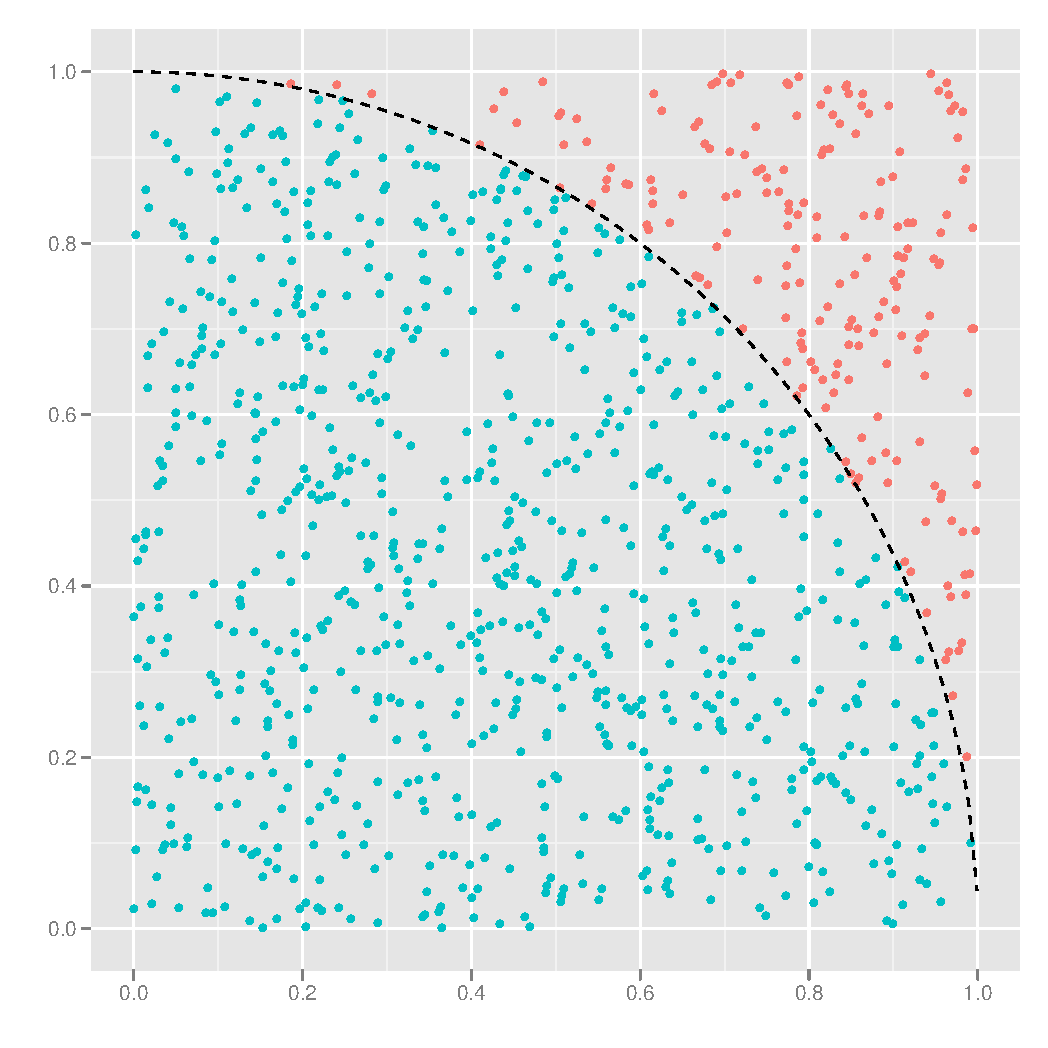
\includegraphics[scale=.25]{pics/pi} 
  \end{center}
  \end{block}
\end{frame}


\begin{frame}[fragile]
  \begin{block}{Example \showex :  Monte Carlo Simulation GBD Algorithm}\pause
    \begin{enumerate}
     \item Let $n$ be big-ish; we'll take $n=50,000$.
     \item Generate an $n\times 2$ matrix $x$ of standard uniform observations.
     \item Count the number of rows satisfying $x^2 + y^2 \leq 1$
     \item Ask everyone else what their answer is; sum it all up.
     \item Take this new answer, multiply by 4 and divide by $n$
     \item If my rank is 0, print the result.
    \end{enumerate}
  \end{block}
\end{frame}


\begin{frame}[fragile,scale,shrink]
  \begin{exampleblock}{Example \showex :  Monte Carlo Simulation Code}\pause
\begin{lstlisting}[title=Serial Code]
N <- 50000
X <- matrix(runif(N * 2), ncol=2)
r <- sum(rowSums(X^2) <= 1)
PI <- 4*r/N
print(PI)
\end{lstlisting}

\begin{lstlisting}[title=Parallel Code]
library(pbdMPI, quiet = TRUE)
init()
comm.set.seed(diff=TRUE)

N.gbd <- 50000 / comm.size()
X.gbd <- matrix(runif(N.gbd * 2), ncol = 2)
r.gbd <- sum(rowSums(X.gbd^2) <= 1)
r <- allreduce(r.gbd)
PI <- 4*r/(N.gbd * comm.size())
comm.print(PI)

finalize()
\end{lstlisting}
  \end{exampleblock}
\end{frame}

\begin{frame}[fragile]
  \begin{block}{Note}\pause
    For the remainder, we will exclude loading, init, and finalize calls.
  \end{block}
\end{frame}










\subsection{pbdMPI Example: Sample Covariance}

\begin{frame}
  \begin{block}{Example \countex :  Sample Covariance}\pause
  \begin{align*}
    cov(x_{n\times p}) = \frac{1}{n-1}\sum_{i=1}^n\left(x_i-\mu_x\right)\left(x_i-\mu_x\right)^T
  \end{align*}
  \end{block}
\end{frame}


\begin{frame}
  \begin{block}{Example \showex :  Sample Covariance GBD Algorithm}\pause
    \begin{enumerate}
     \item Determine the total number of rows $N$.
     \item Compute the vector of column means of the full matrix.
     \item Subtract each column's mean from that column's entries in each local matrix.
     \item Compute the crossproduct locally and reduce.
     \item Divide by $N-1$.
    \end{enumerate}
  \end{block}
\end{frame}


\begin{frame}[fragile,shrink]
  \begin{exampleblock}{Example \showex :  Sample Covariance Code}\pause
\begin{lstlisting}[title=Serial Code]
N <- nrow(X)
mu <- colSums(X) / N

X <- sweep(X, STATS=mu, MARGIN=2)
Cov.X <- crossprod(X) / (N-1)

print(Cov.X)
\end{lstlisting}
  
\begin{lstlisting}[title=Parallel Code]
N <- allreduce(nrow(X.gbd), op="sum")
mu <- allreduce(colSums(X.gbd) / N, op="sum")

X.gbd <- sweep(X.gbd, STATS=mu, MARGIN=2)
Cov.X <- allreduce(crossprod(X.gbd), op="sum") / (N-1)

comm.print(Cov.X)
\end{lstlisting}
  \end{exampleblock}
\end{frame}







\subsection{pbdMPI Example: Linear Regression}

\begin{frame}
  \begin{block}{Example \countex :  Linear Regression}\pause
      Find $\bbeta$ such that
      \begin{align*}
      \by = \bX\bbeta + \bepsilon
      \end{align*}

      When $\bX$ is full rank,
      \begin{align*}
      \hat{\bbeta} = (\bX^T\bX)^{-1}\bX^T\by \label{math:ols}
      \end{align*}
  \end{block}
\end{frame}


\begin{frame}
  \begin{block}{Example \showex :  Linear Regression GBD Algorithm}\pause
    \begin{enumerate}
     \item Locally, compute $tx = x^T$
     \item Locally, compute $A = tx * x$. Query every other processor for this result and sum up all the results.
     \item Locally, compute $B = tx * y$.  Query every other processor for this result and sum up all the results.
     \item Locally, compute $A^{-1} * B$
    \end{enumerate}
  \end{block}
\end{frame}


\begin{frame}[fragile,shrink]
  \begin{exampleblock}{Example \showex :  Linear Regression Code}\pause
\begin{lstlisting}[title=Serial Code]
tX <- t(X)
A <- tX %*% X
B <- tX %*% y

ols <- solve(A) %*% B
\end{lstlisting}
  
\begin{lstlisting}[title=Parallel Code]
tX.gbd <- t(X.gbd)
A <- allreduce(tX.gbd %*% X.gbd, op = "sum")
B <- allreduce(tX.gbd %*% y.gbd, op = "sum")

ols <- solve(A) %*% B
\end{lstlisting}
  \end{exampleblock}
\end{frame}
\begin{frame}
\frametitle{MPI Exercises}
\begin{enumerate}
  \item Experiment with Statistics Examples 1 through 3, running them on 2, 4, and 8 processors.
\end{enumerate}
\end{frame}


\begin{frame}[allowframebreaks=.8]
\frametitle{Advanced MPI Exercises}
\begin{enumerate}
  \item Write a script that will have each processor randomly take a sample of
        size 1 of \code{TRUE} and \code{FALSE}. Have each processor print its
        result.\label{ex:mpi1}

  \item Modify the script in Exercise~\ref{ex:mpi1} above to determine if any
  processors sampled \code{TRUE}. Do the same to determine if all processors 
  sampled \code{TRUE}. In each case, print the result. Compare to the functions 
  \code{comm.all()} and \code{comm.any()}.
  
  \item Generate $50,000,000$ (total) random normal values in parallel on 2, 4, and 8 processors.  Time each run.
  
  %%% GBD
  
  \item Distribute the matrix \code{x <- matrix(1:24, nrow=12)} in GBD format across 4 processors and call it \code{x.spmd}.  
  \begin{enumerate}
    \item Add \code{x.spmd} to itself.
    \item Compute the mean of \code{x.spmd}.
    \item Compute the column means of \code{x.spmd}.
  \end{enumerate}
  
\end{enumerate}
\end{frame}
\section[DMAT]{Introduction to pbdDMAT and the DMAT Structure}

\hidenum
\begin{frame}[noframenumbering]
\frametitle{Contents}
 \tableofcontents[currentsection,hideothersubsections,sectionstyle=show/hide]
\end{frame}
\shownum

\subsection{Introduction to Distributed Matrices}

\begin{frame}
  \begin{block}{Distributed Matrices}\pause
  Most problems in data science are matrix algebra problems, so:
  \begin{center}
  $\text{Distributed matrices} \implies \text{Handle Bigger data}$
  \end{center}
  \end{block}
\end{frame}


\begin{frame}[fragile]
  \begin{block}{Distributed Matrices}\pause
  High level OOP allows \emph{native} serial R syntax:
  \begin{lstlisting}
x <- x[-1, 2:5]
x <- log(abs(x) + 1)
xtx <- t(x) %*% x
ans <- svd(solve(xtx))
  \end{lstlisting}
  \vspace{.4cm}
  However\dots
  \end{block}
\end{frame}


\begin{frame}
  \begin{block}{Distributed Matrices}\pause
  DMAT:
    \begin{itemize}
     \item \textbf{D}istributed \textbf{MAT}rix data structure.
     \item No single processor should hold all of the data.
     \item Block-cyclic matrix distributed across a 2-dimensional grid of processors.
     \item Very robust, but confusing data structure.
    \end{itemize}
  \end{block}
\end{frame}



\begin{frame}
\begin{block}{Distributed Matrices}
\begin{figure}[ht]
        \centering
        \begin{subfigure}[b]{0.3\textwidth}
                \centering
                
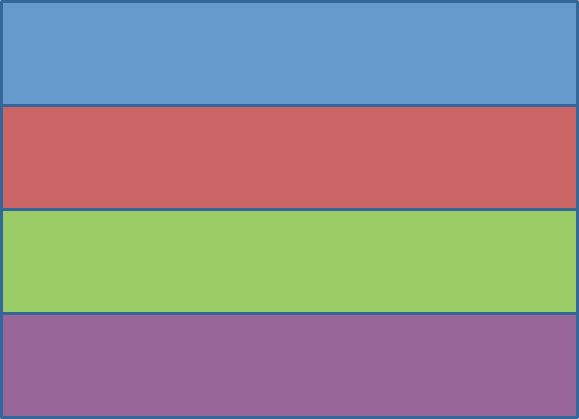
\includegraphics[height=5cm,width=\textwidth]{../common/pics/dmat_block}
                \caption{Block}
        \end{subfigure}
        \hspace{.1cm}
        \begin{subfigure}[b]{0.3\textwidth}
                \centering
                
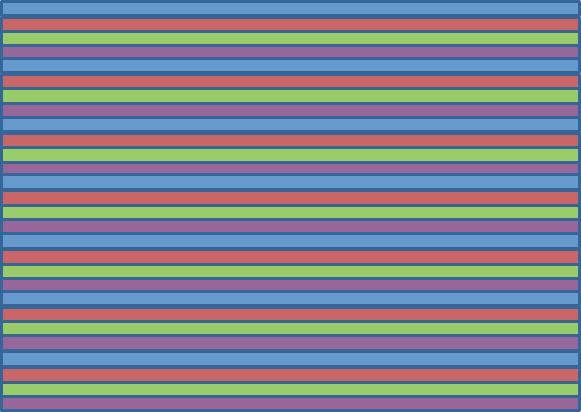
\includegraphics[height=5cm,width=\textwidth]{../common/pics/dmat_cyclic}
                \caption{Cyclic}
        \end{subfigure}
        \hspace{.01cm}
        \begin{subfigure}[b]{0.3\textwidth}
                \centering
                
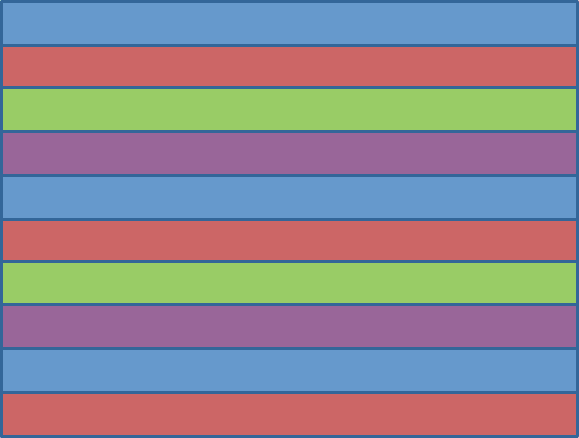
\includegraphics[height=5cm,width=\textwidth]{../common/pics/dmat_blockcyclic}
                \caption{Block-Cyclic}
        \end{subfigure}
        \caption{Matrix Distribution Schemes}\label{fig:dmat1d}
\end{figure}
\end{block}
\end{frame}



\begin{frame}
\begin{block}{Distributed Matrices}
\begin{figure}[ht]
        \centering
        \begin{subfigure}[b]{0.3\textwidth}
                \centering
                
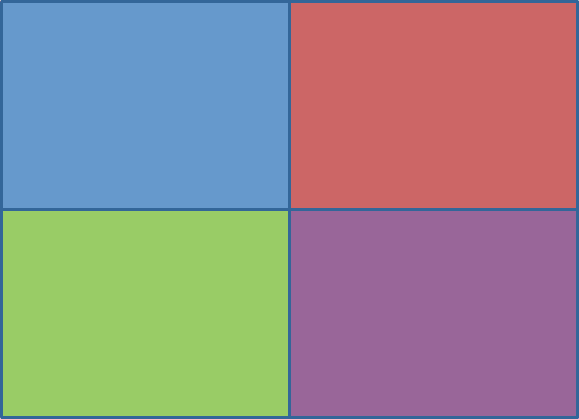
\includegraphics[height=5cm,width=\textwidth]{../common/pics/dmat_block2d}
                \caption{2d Block}
        \end{subfigure}%
        \hspace{.1cm}
        \begin{subfigure}[b]{0.3\textwidth}
                \centering
                
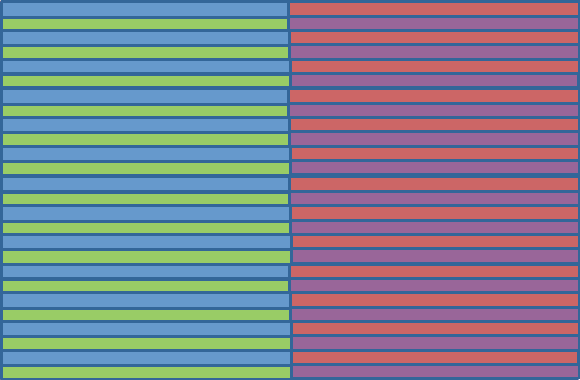
\includegraphics[height=5cm,width=\textwidth]{../common/pics/dmat_cyclic2d}
                \caption{2d Cyclic}
        \end{subfigure}
        \hspace{.01cm}
        \begin{subfigure}[b]{0.3\textwidth}
                \centering
                
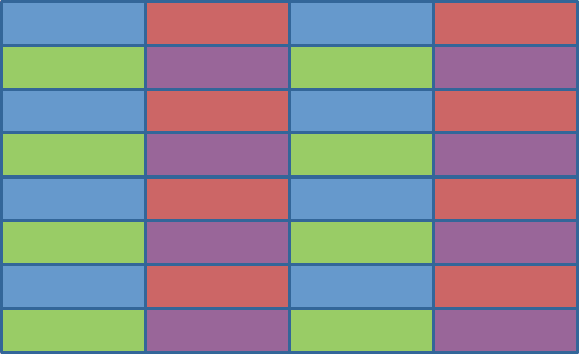
\includegraphics[height=5cm,width=\textwidth]{../common/pics/dmat_blockcyclic2d}
                \caption{2d Block-Cyclic}
        \end{subfigure}
        \caption{Matrix Distribution Schemes Onto a 2-Dimensional 
Grid}\label{fig:dmat2d}
\end{figure}
\end{block}
\end{frame}



\begin{frame}
\begin{block}{Processor Grid Shapes}
\begin{table}[ht]
        \centering
        \begin{subfigure}[b]{0.23\textwidth}
                \centering
              $\left[\begin{tabular}{l}
                  0 \\ 1 \\ 2 \\ 3 \\ 4 \\ 5
                \end{tabular}\right]^T$
                \caption{$1\times 6$}
        \end{subfigure}
        \begin{subfigure}[b]{0.23\textwidth}
                \centering
                $\left[\begin{tabular}{lll}
                  0 & 1 & 2\\
                  3 & 4 & 5
                \end{tabular}\right]$
                \caption{$2\times 3$}
        \end{subfigure}%
        \begin{subfigure}[b]{0.23\textwidth}
                \centering
              $\left[\begin{tabular}{ll}
                  0 & 1 \\
                  2 & 3\\
                  4 & 5
                \end{tabular}\right]$
                \caption{$3\times 2$}
        \end{subfigure}
        \begin{subfigure}[b]{0.23\textwidth}
                \centering
              $\left[\begin{tabular}{l}
                  0 \\ 1 \\ 2 \\ 3 \\ 4 \\ 5
                \end{tabular}\right]$
                \caption{$6\times 1$}
        \end{subfigure}
        \caption{Processor Grid Shapes with 6 Processors}\label{fig:gridshapes}
\end{table}
\end{block}
\end{frame}





\begin{frame}
  \begin{block}{Distributed Matrices}\pause
  The data structure is a special R class (in the OOP sense) called 
\code{ddmatrix}.  It is the ``under the rug'' storage for a block-cyclic matrix 
distributed onto a 2-dimensional processor grid.\\[.4cm]
{\tiny
\begin{align*}
\hspace{.1cm}\text{\code{ddmatrix}}&=\begin{cases}
 $\textbf{Data}$ & $S4 local submatrix, an R matrix$\\
 $\textbf{dim}$ & $S4 dimension of the global matrix, a numeric pair$\\
 $\textbf{ldim}$ & $S4 dimension of the local submatrix, a numeric pair$\\
 $\textbf{bldim}$ & $S4 ScaLAPACK blocking factor, a numeric pair$\\
 $\textbf{CTXT}$ & $S4 BLACS context, an numeric singleton$
 \end{cases}
\end{align*}
}with prototype{\tiny
\begin{align*}
\hspace{-2.9cm}\text{\code{new("ddmatrix")}}&=\begin{cases}
 $\textbf{Data}$ & =\text{\code{matrix(0.0)}}\\
 $\textbf{dim}$ & =\text{\code{c(1,1)}}\\
 $\textbf{ldim}$ & =\text{\code{c(1,1)}}\\
 $\textbf{bldim}$ & =\text{\code{c(1,1)}}\\
 $\textbf{CTXT}$ & =\text{\code{0.0}}
 \end{cases}
\end{align*}
}
  \end{block}
\end{frame}


\begin{frame}
  \begin{block}{Distributed Matrices:  The Data Structure}\pause
      Example:  an $9\times 9$ matrix is distributed with a ``block-cycling'' 
factor of $2\times 2$ on a $2\times 2$ processor grid:
      \begin{center}
      \begin{minipage}{.45\textwidth}
      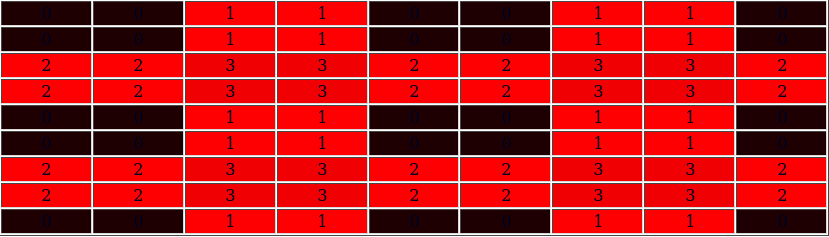
\includegraphics[width=5cm, height=4cm]{../common/pics/dmat_dist}  
      \end{minipage}\hspace{.1cm}
      \begin{minipage}{.45\textwidth}
      \begin{center}
      \begin{align*}
        &=\begin{cases}
        $\textbf{Data}$ & =\text{\code{matrix(\dots)}}\\
        $\textbf{dim}$ & =\text{\code{c(9, 9)}}\\
        $\textbf{ldim}$ & =\text{\code{c(\dots)}}\\
        $\textbf{bldim}$ & =\text{\code{c(2, 2)}}\\
        $\textbf{CTXT}$ & =0
        \end{cases}
        \end{align*}
      \end{center}
      \end{minipage}
      \end{center}
    {\small See \url{http://acts.nersc.gov/scalapack/hands-on/datadist.html}}
  \end{block}
\end{frame}

  
  
  

\subsection{DMAT Distributions}




\begin{frame}
\begin{exampleblock}{Understanding Dmat: Global Matrix}
\begin{align*}
x &= \left[
      \begin{array}{lllllllll}
      x_{11} & x_{12} & x_{13} & x_{14} & x_{15} & x_{16} & x_{17} & x	_{18} & x_{19}\\
      x_{21} & x_{22} & x_{23} & x_{24} & x_{25} & x_{26} & x_{27} & x	_{28} & x_{29}\\
      x_{31} & x_{32} & x_{33} & x_{34} & x_{35} & x_{36} & x_{37} & x	_{38} & x_{39}\\
      x_{41} & x_{42} & x_{43} & x_{44} & x_{45} & x_{46} & x_{47} & x	_{48} & x_{49}\\
      x_{51} & x_{52} & x_{53} & x_{54} & x_{55} & x_{56} & x_{57} & x	_{58} & x_{59}\\
      x_{61} & x_{62} & x_{63} & x_{64} & x_{65} & x_{66} & x_{67} & x	_{68} & x_{69}\\
      x_{71} & x_{72} & x_{73} & x_{74} & x_{75} & x_{76} & x_{77} & x	_{78} & x_{79}\\
      x_{81} & x_{82} & x_{83} & x_{84} & x_{85} & x_{86} & x_{87} & x	_{88} & x_{89}\\
      x_{91} & x_{92} & x_{93} & x_{94} & x_{95} & x_{96} & x_{97} & x	_{98} & x_{99}
      \end{array}
\right]_{9\times 9}
\end{align*}
\end{exampleblock}
\end{frame}



\begin{frame}
\begin{exampleblock}{DMAT:  1-dimensional Row Block}
\begin{align*}
x &= \left[
      \begin{array}{lllllllll}
      \color{g11}x_{11} & \color{g11}x_{12} & \color{g11}x_{13} & 
\color{g11}x_{14} & \color{g11}x_{15} & \color{g11}x_{16} & \color{g11}x_{17} & 
\color{g11}x_{18} & \color{g11}x_{19}\\
      \color{g11}x_{21} & \color{g11}x_{22} & \color{g11}x_{23} & 
\color{g11}x_{24} & \color{g11}x_{25} & \color{g11}x_{26} & \color{g11}x_{27} & 
\color{g11}x_{28} & \color{g11}x_{29}\\
      \color{g11}x_{31} & \color{g11}x_{32} & \color{g11}x_{33} & 
\color{g11}x_{34} & \color{g11}x_{35} & \color{g11}x_{36} & \color{g11}x_{37} & 
\color{g11}x_{38} & \color{g11}x_{39}\\\hline
      \color{g12}x_{41} & \color{g12}x_{42} & \color{g12}x_{43} & 
\color{g12}x_{44} & \color{g12}x_{45} & \color{g12}x_{46} & \color{g12}x_{47} & 
\color{g12}x_{48} & \color{g12}x_{49}\\
      \color{g12}x_{51} & \color{g12}x_{52} & \color{g12}x_{53} & 
\color{g12}x_{54} & \color{g12}x_{55} & \color{g12}x_{56} & \color{g12}x_{57} & 
\color{g12}x_{58} & \color{g12}x_{59}\\
      \color{g12}x_{61} & \color{g12}x_{62} & \color{g12}x_{63} & 
\color{g12}x_{64} & \color{g12}x_{65} & \color{g12}x_{66} & \color{g12}x_{67} & 
\color{g12}x_{68} & \color{g12}x_{69}\\\hline
      \color{g13}x_{71} & \color{g13}x_{72} & \color{g13}x_{73} & 
\color{g13}x_{74} & \color{g13}x_{75} & \color{g13}x_{76} & \color{g13}x_{77} & 
\color{g13}x_{78} & \color{g13}x_{79}\\
      \color{g13}x_{81} & \color{g13}x_{82} & \color{g13}x_{83} & 
\color{g13}x_{84} & \color{g13}x_{85} & \color{g13}x_{86} & \color{g13}x_{87} & 
\color{g13}x_{88} & \color{g13}x_{89}\\
      \color{g13}x_{91} & \color{g13}x_{92} & \color{g13}x_{93} & 
\color{g13}x_{94} & \color{g13}x_{95} & \color{g13}x_{96} & \color{g13}x_{97} & 
\color{g13}x_{98} & \color{g13}x_{99}\\
      \end{array}
\right]_{9\times 9}
\end{align*}
\vspace{-.6cm}
\begin{align*}
\text{Processor grid = }\left|
      \begin{array}{l}
      \color{g11}0 \\
      \color{g12}1 \\
      \color{g13}2 \\
      \color{g21}3
      \end{array}
\right| &= 
\left|
      \begin{tabular}{l}
      \color{g11}(0,0) \\
      \color{g12}(0,1) \\
      \color{g13}(1,0) \\
      \color{g21}(1,1) 
      \end{tabular}
\right|
\end{align*}
\end{exampleblock}
\end{frame}





\begin{frame}
\begin{exampleblock}{DMAT: 2-dimensional Row Block}
\begin{align*}
x &= \left[
      \begin{array}{lllll|llll}
      \color{g11}x_{11} & \color{g11}x_{12} & \color{g11}x_{13} & 
\color{g11}x_{14} & \color{g11}x_{15} & \color{g12}x_{16} & \color{g12}x_{17} & 
\color{g12}x_{18} & \color{g12}x_{19}\\
      \color{g11}x_{21} & \color{g11}x_{22} & \color{g11}x_{23} & 
\color{g11}x_{24} & \color{g11}x_{25} & \color{g12}x_{26} & \color{g12}x_{27} & 
\color{g12}x_{28} & \color{g12}x_{29}\\
      \color{g11}x_{31} & \color{g11}x_{32} & \color{g11}x_{33} & 
\color{g11}x_{34} & \color{g11}x_{35} & \color{g12}x_{36} & \color{g12}x_{37} & 
\color{g12}x_{38} & \color{g12}x_{39}\\
      \color{g11}x_{41} & \color{g11}x_{42} & \color{g11}x_{43} & 
\color{g11}x_{44} & \color{g11}x_{45} & \color{g12}x_{46} & \color{g12}x_{47} & 
\color{g12}x_{48} & \color{g12}x_{49}\\
      \color{g11}x_{51} & \color{g11}x_{52} & \color{g11}x_{53} & 
\color{g11}x_{54} & \color{g11}x_{55} & \color{g12}x_{56} & \color{g12}x_{57} & 
\color{g12}x_{58} & \color{g12}x_{59}\\\hline
      \color{g13}x_{61} & \color{g13}x_{62} & \color{g13}x_{63} & 
\color{g13}x_{64} & \color{g13}x_{65} & \color{g21}x_{66} & \color{g21}x_{67} & 
\color{g21}x_{68} & \color{g21}x_{69}\\
      \color{g13}x_{71} & \color{g13}x_{72} & \color{g13}x_{73} & 
\color{g13}x_{74} & \color{g13}x_{75} & \color{g21}x_{76} & \color{g21}x_{77} & 
\color{g21}x_{78} & \color{g21}x_{79}\\
      \color{g13}x_{81} & \color{g13}x_{82} & \color{g13}x_{83} & 
\color{g13}x_{84} & \color{g13}x_{85} & \color{g21}x_{86} & \color{g21}x_{87} & 
\color{g21}x_{88} & \color{g21}x_{89}\\
      \color{g13}x_{91} & \color{g13}x_{92} & \color{g13}x_{93} & 
\color{g13}x_{94} & \color{g13}x_{95} & \color{g21}x_{96} & \color{g21}x_{97} & 
\color{g21}x_{98} & \color{g21}x_{99}\\
      \end{array}
\right]_{9\times 9}
\end{align*}
\begin{align*}
\text{Processor grid = }\left|
      \begin{array}{ll}
      \color{g11}0 & \color{g12}1 \\
      \color{g13}2 & \color{g21}3
      \end{array}
\right| &= 
\left|
      \begin{tabular}{lll}
      \color{g11}(0,0) & \color{g12}(0,1) \\
      \color{g13}(1,0) & \color{g21}(1,1) 
      \end{tabular}
\right|
\end{align*}
\end{exampleblock}
\end{frame}



\begin{frame}
\begin{exampleblock}{DMAT: 1-dimensional Row Cyclic}
\begin{align*}
x &= \left[
      \begin{array}{lllllllll}
      \color{g11}x_{11} & \color{g11}x_{12} & \color{g11}x_{13} & 
\color{g11}x_{14} & \color{g11}x_{15} & \color{g11}x_{16} & \color{g11}x_{17} & 
\color{g11}x_{18} & \color{g11}x_{19}\\\hline
      \color{g12}x_{21} & \color{g12}x_{22} & \color{g12}x_{23} & 
\color{g12}x_{24} & \color{g12}x_{25} & \color{g12}x_{26} & \color{g12}x_{27} & 
\color{g12}x_{28} & \color{g12}x_{29}\\\hline
      \color{g13}x_{31} & \color{g13}x_{32} & \color{g13}x_{33} & 
\color{g13}x_{34} & \color{g13}x_{35} & \color{g13}x_{36} & \color{g13}x_{37} & 
\color{g13}x_{38} & \color{g13}x_{39}\\\hline
      \color{g21}x_{41} & \color{g21}x_{42} & \color{g21}x_{43} & 
\color{g21}x_{44} & \color{g21}x_{45} & \color{g21}x_{46} & \color{g21}x_{47} & 
\color{g21}x_{48} & \color{g21}x_{49}\\\hline
      \color{g11}x_{51} & \color{g11}x_{52} & \color{g11}x_{53} & 
\color{g11}x_{54} & \color{g11}x_{55} & \color{g11}x_{56} & \color{g11}x_{57} & 
\color{g11}x_{58} & \color{g11}x_{59}\\\hline
      \color{g12}x_{61} & \color{g12}x_{62} & \color{g12}x_{63} & 
\color{g12}x_{64} & \color{g12}x_{65} & \color{g12}x_{66} & \color{g12}x_{67} & 
\color{g12}x_{68} & \color{g12}x_{69}\\\hline
      \color{g13}x_{71} & \color{g13}x_{72} & \color{g13}x_{73} & 
\color{g13}x_{74} & \color{g13}x_{75} & \color{g13}x_{76} & \color{g13}x_{77} & 
\color{g13}x_{78} & \color{g13}x_{79}\\\hline
      \color{g21}x_{81} & \color{g21}x_{82} & \color{g21}x_{83} & 
\color{g21}x_{84} & \color{g21}x_{85} & \color{g21}x_{86} & \color{g21}x_{87} & 
\color{g21}x_{88} & \color{g21}x_{89}\\\hline
      \color{g11}x_{91} & \color{g11}x_{92} & \color{g11}x_{93} & 
\color{g11}x_{94} & \color{g11}x_{95} & \color{g11}x_{96} & \color{g11}x_{97} & 
\color{g11}x_{98} & \color{g11}x_{99}\\
      \end{array}
\right]_{9\times 9}
\end{align*}
\vspace{-.6cm}
\begin{align*}
\text{Processor grid = }\left|
      \begin{array}{l}
      \color{g11}0 \\
      \color{g12}1 \\
      \color{g13}2 \\
      \color{g21}3
      \end{array}
\right| &= 
\left|
      \begin{tabular}{lll}
      \color{g11}(0,0) \\
      \color{g12}(0,1) \\
      \color{g13}(1,0) \\
      \color{g21}(1,1) 
      \end{tabular}
\right|
\end{align*}
\end{exampleblock}
\end{frame}



\begin{frame}
\begin{exampleblock}{DMAT: 2-dimensional Row Cyclic}
\begin{align*}
x &= \left[
      \begin{array}{lllll|llll}
      \color{g11}x_{11} & \color{g11}x_{12} & \color{g11}x_{13} & 
\color{g11}x_{14} & \color{g11}x_{15} & \color{g12}x_{16} & \color{g12}x_{17} & 
\color{g12}x_{18} & \color{g12}x_{19}\\\hline
      \color{g13}x_{21} & \color{g13}x_{22} & \color{g13}x_{23} & 
\color{g13}x_{24} & \color{g13}x_{25} & \color{g21}x_{26} & \color{g21}x_{27} & 
\color{g21}x_{28} & \color{g21}x_{29}\\\hline
      \color{g11}x_{31} & \color{g11}x_{32} & \color{g11}x_{33} & 
\color{g11}x_{34} & \color{g11}x_{35} & \color{g12}x_{36} & \color{g12}x_{37} & 
\color{g12}x_{38} & \color{g12}x_{39}\\\hline
      \color{g13}x_{41} & \color{g13}x_{42} & \color{g13}x_{43} & 
\color{g13}x_{44} & \color{g13}x_{45} & \color{g21}x_{46} & \color{g21}x_{47} & 
\color{g21}x_{48} & \color{g21}x_{49}\\\hline
      \color{g11}x_{51} & \color{g11}x_{52} & \color{g11}x_{53} & 
\color{g11}x_{54} & \color{g11}x_{55} & \color{g12}x_{56} & \color{g12}x_{57} & 
\color{g12}x_{58} & \color{g12}x_{59}\\\hline
      \color{g13}x_{61} & \color{g13}x_{62} & \color{g13}x_{63} & 
\color{g13}x_{64} & \color{g13}x_{65} & \color{g21}x_{66} & \color{g21}x_{67} & 
\color{g21}x_{68} & \color{g21}x_{69}\\\hline
      \color{g11}x_{71} & \color{g11}x_{72} & \color{g11}x_{73} & 
\color{g11}x_{74} & \color{g11}x_{75} & \color{g12}x_{76} & \color{g12}x_{77} & 
\color{g12}x_{78} & \color{g12}x_{79}\\\hline
      \color{g13}x_{81} & \color{g13}x_{82} & \color{g13}x_{83} & 
\color{g13}x_{84} & \color{g13}x_{85} & \color{g21}x_{86} & \color{g21}x_{87} & 
\color{g21}x_{88} & \color{g21}x_{89}\\\hline
      \color{g11}x_{91} & \color{g11}x_{92} & \color{g11}x_{93} & 
\color{g11}x_{94} & \color{g11}x_{95} & \color{g12}x_{96} & \color{g12}x_{97} & 
\color{g12}x_{98} & \color{g12}x_{99}\\
      \end{array}
\right]_{9\times 9}
\end{align*}
\begin{align*}
\text{Processor grid = }\left|
      \begin{array}{ll}
      \color{g11}0 & \color{g12}1 \\
      \color{g13}2 & \color{g21}3
      \end{array}
\right| &= 
\left|
      \begin{tabular}{lll}
      \color{g11}(0,0) & \color{g12}(0,1) \\
      \color{g13}(1,0) & \color{g21}(1,1) 
      \end{tabular}
\right|
\end{align*}
\end{exampleblock}
\end{frame}




\begin{frame}[shrink]
\begin{exampleblock}{DMAT: 2-dimensional Block-Cyclic}
\begin{align*}
x &= \left[
      \begin{array}{ll|ll|ll|ll|l}
      \color{g11}x_{11} & \color{g11}x_{12} & \color{g12}x_{13} & \color{g12}x_{14} & \color{g11}x_{15} & \color{g11}x_{16} & \color{g12}x_{17} & \color{g12}x_{18} & \color{g11}x_{19}\\
      \color{g11}x_{21} & \color{g11}x_{22} & \color{g12}x_{23} & \color{g12}x_{24} & \color{g11}x_{25} & \color{g11}x_{26} & \color{g12}x_{27} & \color{g12}x_{28} & \color{g11}x_{29}\\\hline
      \color{g13}x_{31} & \color{g13}x_{32} & \color{g21}x_{33} & \color{g21}x_{34} & \color{g13}x_{35} & \color{g13}x_{36} & \color{g21}x_{37} & \color{g21}x_{38} & \color{g13}x_{39}\\
      \color{g13}x_{41} & \color{g13}x_{42} & \color{g21}x_{43} & \color{g21}x_{44} & \color{g13}x_{45} & \color{g13}x_{46} & \color{g21}x_{47} & \color{g21}x_{48} & \color{g13}x_{49}\\\hline
      \color{g11}x_{51} & \color{g11}x_{52} & \color{g12}x_{53} & \color{g12}x_{54} & \color{g11}x_{55} & \color{g11}x_{56} & \color{g12}x_{57} & \color{g12}x_{58} & \color{g11}x_{59}\\
      \color{g11}x_{61} & \color{g11}x_{62} & \color{g12}x_{63} & \color{g12}x_{64} & \color{g11}x_{65} & \color{g11}x_{66} & \color{g12}x_{67} & \color{g12}x_{68} & \color{g11}x_{69}\\\hline
      \color{g13}x_{71} & \color{g13}x_{72} & \color{g21}x_{73} & \color{g21}x_{74} & \color{g13}x_{75} & \color{g13}x_{76} & \color{g21}x_{77} & \color{g21}x_{78} & \color{g13}x_{79}\\
      \color{g13}x_{81} & \color{g13}x_{82} & \color{g21}x_{83} & \color{g21}x_{84} & \color{g13}x_{85} & \color{g13}x_{86} & \color{g21}x_{87} & \color{g21}x_{88} & \color{g13}x_{89}\\\hline
      \color{g11}x_{91} & \color{g11}x_{92} & \color{g12}x_{93} & \color{g12}x_{94} & \color{g11}x_{95} & \color{g11}x_{96} & \color{g12}x_{97} & \color{g12}x_{98} & \color{g11}x_{99}\\
      \end{array}
\right]_{9\times 9}
\end{align*}
\begin{align*}
\text{Processor grid = }\left|
      \begin{array}{ll}
      \color{g11}0 & \color{g12}1 \\
      \color{g13}2 & \color{g21}3
      \end{array}
\right| &= 
\left|
      \begin{tabular}{lll}
      \color{g11}(0,0) & \color{g12}(0,1) \\
      \color{g13}(1,0) & \color{g21}(1,1) 
      \end{tabular}
\right|
\end{align*}
\end{exampleblock}
\end{frame}








\subsection{pbdDMAT}

\begin{frame}[fragile]
  \begin{block}{The \code{DMAT} Data Structure}\pause
    The more complicated the processor grid, the more complicated the distribution.
  \end{block}
\end{frame}


\begin{frame}[shrink]
\begin{exampleblock}{DMAT: 2-dimensional Block-Cyclic with 6 Processors}
\begin{align*}
x &= \left[
      \begin{array}{ll|ll|ll|ll|l}
      \color{g11}x_{11} & \color{g11}x_{12} & \color{g12}x_{13} & \color{g12}x_{14} & \color{g13}x_{15} & \color{g13}x_{16} & \color{g11}x_{17} & \color{g11}x_{18} & \color{g12}x_{19}\\
      \color{g11}x_{21} & \color{g11}x_{22} & \color{g12}x_{23} & \color{g12}x_{24} & \color{g13}x_{25} & \color{g13}x_{26} & \color{g11}x_{27} & \color{g11}x_{28} & \color{g12}x_{29}\\\hline
      \color{g21}x_{31} & \color{g21}x_{32} & \color{g22}x_{33} & \color{g22}x_{34} & \color{g23}x_{35} & \color{g23}x_{36} & \color{g21}x_{37} & \color{g21}x_{38} & \color{g22}x_{39}\\
      \color{g21}x_{41} & \color{g21}x_{42} & \color{g22}x_{43} & \color{g22}x_{44} & \color{g23}x_{45} & \color{g23}x_{46} & \color{g21}x_{47} & \color{g21}x_{48} & \color{g22}x_{49}\\\hline
      \color{g11}x_{51} & \color{g11}x_{52} & \color{g12}x_{53} & \color{g12}x_{54} & \color{g13}x_{55} & \color{g13}x_{56} & \color{g11}x_{57} & \color{g11}x_{58} & \color{g12}x_{59}\\
      \color{g11}x_{61} & \color{g11}x_{62} & \color{g12}x_{63} & \color{g12}x_{64} & \color{g13}x_{65} & \color{g13}x_{66} & \color{g11}x_{67} & \color{g11}x_{68} & \color{g12}x_{69}\\\hline
      \color{g21}x_{71} & \color{g21}x_{72} & \color{g22}x_{73} & \color{g22}x_{74} & \color{g23}x_{75} & \color{g23}x_{76} & \color{g21}x_{77} & \color{g21}x_{78} & \color{g22}x_{79}\\
      \color{g21}x_{81} & \color{g21}x_{82} & \color{g22}x_{83} & \color{g22}x_{84} & \color{g23}x_{85} & \color{g23}x_{86} & \color{g21}x_{87} & \color{g21}x_{88} & \color{g22}x_{89}\\\hline
      \color{g11}x_{91} & \color{g11}x_{92} & \color{g12}x_{93} & \color{g12}x_{94} & \color{g13}x_{95} & \color{g13}x_{96} & \color{g11}x_{97} & \color{g11}x_{98} & \color{g12}x_{99}\\
      \end{array}
\right]_{9\times 9}
\end{align*}
\begin{align*}
\text{Processor grid = }\left|
      \begin{array}{lll}
      \color{g11}0 & \color{g12}1 & \color{g13}2\\
      \color{g21}3 & \color{g22}4 & \color{g23}5
      \end{array}
\right| &= 
\left|
      \begin{tabular}{lll}
      \color{g11}(0,0) & \color{g12}(0,1) & \color{g13}(0,2)\\
      \color{g21}(1,0) & \color{g22}(1,1) & \color{g23}(1,2)
      \end{tabular}
\right|
\end{align*}
\end{exampleblock}
\end{frame}


\begin{frame}[shrink]
\begin{exampleblock}{Understanding DMAT: Local View}
\begin{align*}
\left[
      \begin{array}{ll|ll}
      \color{g11}x_{11} & \color{g11}x_{12} & \color{g11}x_{17} & \color{g11}x_{18}\\
      \color{g11}x_{21} & \color{g11}x_{22} & \color{g11}x_{27} & \color{g11}x_{28}\\\hline
      \color{g11}x_{51} & \color{g11}x_{52} & \color{g11}x_{57} & \color{g11}x_{58}\\
      \color{g11}x_{61} & \color{g11}x_{62} & \color{g11}x_{67} & \color{g11}x_{68}\\\hline
      \color{g11}x_{91} & \color{g11}x_{92} & \color{g11}x_{97} & \color{g11}x_{98}\\
      \end{array}
\right]_{5\times 4}
\left[
      \begin{array}{ll|l}
      \color{g12}x_{13} & \color{g12}x_{14} & \color{g12}x_{19}\\
      \color{g12}x_{23} & \color{g12}x_{24} & \color{g12}x_{29}\\\hline
      \color{g12}x_{53} & \color{g12}x_{54} & \color{g12}x_{59}\\
      \color{g12}x_{63} & \color{g12}x_{64} & \color{g12}x_{69}\\\hline
      \color{g12}x_{93} & \color{g12}x_{94} & \color{g12}x_{99}\\
      \end{array}
\right]_{5\times 3}
\left[
      \begin{array}{ll}
      \color{g13}x_{15} & \color{g13}x_{16}\\
      \color{g13}x_{25} & \color{g13}x_{26}\\\hline
      \color{g13}x_{55} & \color{g13}x_{56}\\
      \color{g13}x_{65} & \color{g13}x_{66}\\\hline
      \color{g13}x_{95} & \color{g13}x_{96}\\
      \end{array}
\right]_{5\times 2}
\\
\left[
      \begin{array}{ll|ll}
      \color{g21}x_{31} & \color{g21}x_{32} & \color{g21}x_{37} & \color{g21}x_{38}\\
      \color{g21}x_{41} & \color{g21}x_{42} & \color{g21}x_{47} & \color{g21}x_{48}\\\hline
      \color{g21}x_{71} & \color{g21}x_{72} & \color{g21}x_{77} & \color{g21}x_{78}\\
      \color{g21}x_{81} & \color{g21}x_{82} & \color{g21}x_{87} & \color{g21}x_{88}\\
      \end{array}
\right]_{4\times 4}
\left[
      \begin{array}{ll|l}
      \color{g22}x_{33} & \color{g22}x_{34} & \color{g22}x_{39}\\
      \color{g22}x_{43} & \color{g22}x_{44} & \color{g22}x_{49}\\\hline
      \color{g22}x_{73} & \color{g22}x_{74} & \color{g22}x_{79}\\
      \color{g22}x_{83} & \color{g22}x_{84} & \color{g22}x_{89}\\
      \end{array}
\right]_{4\times 3}
\left[
      \begin{array}{ll}
      \color{g23}x_{35} & \color{g23}x_{36} \\
      \color{g23}x_{45} & \color{g23}x_{46} \\\hline
      \color{g23}x_{75} & \color{g23}x_{76} \\
      \color{g23}x_{85} & \color{g23}x_{86} \\
      \end{array}
\right]_{4\times 2}
\end{align*}
\begin{align*}
\text{Processor grid = }\left|
      \begin{array}{lll}
      \color{g11}0 & \color{g12}1 & \color{g13}2\\
      \color{g21}3 & \color{g22}4 & \color{g23}5
      \end{array}
\right| &= 
\left|
      \begin{tabular}{lll}
      \color{g11}(0,0) & \color{g12}(0,1) & \color{g13}(0,2)\\
      \color{g21}(1,0) & \color{g22}(1,1) & \color{g23}(1,2)
      \end{tabular}
\right|
\end{align*}
\end{exampleblock}
\end{frame}



\begin{frame}[fragile]
  \fontsize{8pt}{10}\selectfont
  \begin{block}{The \code{DMAT} Data Structure}\pause
  \begin{columns}[c,onlytextwidth]
    \begin{column}{0.59\textwidth}
      \begin{enumerate}
        \item \code{DMAT} is \emph{distributed}.  No one processor owns all of the matrix.
        \item \code{DMAT} is \emph{non-overlapping}. Any piece owned by one processor is owned by no other processors.\\\hrule
        \item \code{DMAT} can be row-contiguous or not, depending on the processor grid and blocking factor used.
        \item \code{DMAT} is locally column-major and globally, it depends\dots
      \end{enumerate}
    \end{column}
    \begin{column}{0.4\textwidth}
      \begin{align*}
\left[
      \begin{array}{ll|ll|l}
      \color{g11}x_{11} & \color{g11}x_{12} & \color{g12}x_{13} & \color{g12}x_{14} & \color{g13}x_{15} \\
      \color{g11}x_{21} & \color{g11}x_{22} & \color{g12}x_{23} & \color{g12}x_{24} & \color{g13}x_{25} \\\hline
      \color{g21}x_{31} & \color{g21}x_{32} & \color{g22}x_{33} & \color{g22}x_{34} & \color{g23}x_{35} \\
      \color{g21}x_{41} & \color{g21}x_{42} & \color{g22}x_{43} & \color{g22}x_{44} & \color{g23}x_{45} \\\hline
      \color{g11}x_{51} & \color{g11}x_{52} & \color{g12}x_{53} & \color{g12}x_{54} & \color{g13}x_{55} \\
      \color{g11}x_{61} & \color{g11}x_{62} & \color{g12}x_{63} & \color{g12}x_{64} & \color{g13}x_{65} \\\hline
      \color{g21}x_{71} & \color{g21}x_{72} & \color{g22}x_{73} & \color{g22}x_{74} & \color{g23}x_{75} \\
      \color{g21}x_{81} & \color{g21}x_{82} & \color{g22}x_{83} & \color{g22}x_{84} & \color{g23}x_{85} \\\hline
      \color{g11}x_{91} & \color{g11}x_{92} & \color{g12}x_{93} & \color{g12}x_{94} & \color{g13}x_{95} \\
      \end{array}
      \right]
      \end{align*}
    \end{column}
  \end{columns}
  \begin{enumerate}
    \setcounter{enumi}{5}
        \item \code{GBD} is a generalization of the one-dimensional block \code{DMAT} distribution.  Otherwise there is no relation.
        \item \code{DMAT} is confusing, but very robust.
    \end{enumerate}
  \end{block}
\end{frame}












\begin{frame}
  \begin{block}{Pros and Cons of This Data Structure}\pause
  \begin{center}
    \begin{minipage}[t]{.45\textwidth}
      \begin{center}
      \begin{block}{Pros}
	\begin{itemize}
	\item Fast for distributed matrix computations
	\end{itemize}
      \end{block}
      \end{center}
    \end{minipage}\hspace{.5cm}
    \begin{minipage}[t]{.45\textwidth}
      \begin{center}
      \begin{block}{Cons}
	\begin{itemize}
	  \item Literally everything else
	\end{itemize}
      \end{block}
      \end{center}
    \end{minipage}
    \\[.6cm]
    \emph{This is why we hide most of the distributed details.}
    \\[.4cm]
    The details are there if you want them (you don't want them).
  \end{center}
  \end{block}
\end{frame}


\begin{frame}[fragile]
  \begin{block}{Distributed Matrix Methods}\pause
    \pkg{pbdDMAT} has over 100 methods with \emph{identical} syntax to R:
    \begin{itemize}
     \item \code{\`{}[\`{}}, \code{rbind()}, \code{cbind()}, \dots
     \item \code{lm.fit()}, \code{prcomp()}, \code{cov()}, \dots
     \item \code{\`{}\%*\%\`{}}, \code{solve()}, \code{svd()}, \code{norm()}, \dots
     \item \code{median()}, \code{mean()}, \code{rowSums()}, \dots
    \end{itemize}
\begin{lstlisting}[title=Serial Code]
cov(x)
\end{lstlisting}
  
\begin{lstlisting}[title=Parallel Code]
cov(x)
\end{lstlisting}
  \end{block}
\end{frame}

\begin{frame}[fragile]
  \begin{block}{Comparing pbdMPI and pbdDMAT}\pause
\pkg{pbdMPI}:
  \begin{itemize}
     \item MPI $+$ sugar.
     \item \code{GBD} not the only structure \pkg{pbdMPI} can handle (just a useful convention).
     \end{itemize}
     
     \pkg{pbdDMAT}:
     \begin{itemize}
     \item More of a software package.
     \item \code{DMAT} structure \emph{must} be used for \pkg{pbdDMAT}.
     \item If the data is not 2d block-cyclic compatible, DMAT will \emph{definitely} give the wrong answer.
    \end{itemize}
  \end{block}
\end{frame}

\begin{frame}[fragile]
  \begin{block}{Quick Comments for Using pbdDMAT}\pause
    \begin{enumerate}
      \item Start by loading the package:
\vspace{-.4cm}
\begin{lstlisting}
library(pbdDMAT, quiet = TRUE)
\end{lstlisting}
      \item Always initialize before starting and finalize when finished:
\vspace{-.4cm}
\begin{lstlisting}
init.grid()

# ...

finalize()
\end{lstlisting}
      \item   Distributed \code{DMAT} objects will be given the suffix \code{.dmat} to visually help distinguish them from global objects.  This suffix carries no semantic meaning.
    \end{enumerate}
  \end{block}
\end{frame}


\section[pbdDMAT eg's]{Examples Using pbdDMAT}
\setcounter{excount}{0}


\hidenum
\begin{frame}[noframenumbering]
\frametitle{Contents}
 \tableofcontents[currentsection,hideothersubsections,sectionstyle=show/hide]
\end{frame}
\shownum

% 
% 
% \subsection{Manipulating DMAT Objects}
% 
% \begin{frame}[fragile,shrink]
%   \begin{exampleblock}{Example \countex:  DMAT Construction}\pause
% \begin{lstlisting}[title=Generate a global matrix and distribute it]
% library(pbdDMAT, quiet=TRUE)
% init.grid()
% 
% # Common global on all processors --> distributed
% x <- matrix(1:100, nrow=10, ncol=10)
% x.dmat <- as.ddmatrix(x)
% 
% x.dmat
% 
% # Global on processor 0 --> distributed
% if (comm.rank()==0){
%   y <- matrix(1:100, nrow=10, ncol=10)
% } else {
%   y <- NULL
% }
% y.dmat <- as.ddmatrix(y)
% 
% y.dmat
% 
% finalize()
% \end{lstlisting}
% \begin{lstlisting}[basicstyle=\tiny,backgroundcolor=\color{white},keywordstyle=\color{black},title=\fontsize{6pt}{7.2}\selectfont Execute this script via:]
% mpirun -np 2 Rscript 1_gen.r
% \end{lstlisting} 
%   \end{exampleblock}
% \end{frame}
% 
% 
% 
% \begin{frame}[fragile]
%   \begin{exampleblock}{Example \countex:  DMAT Construction}\pause
% \begin{lstlisting}[title=Generate locally only what is needed]
% library(pbdDMAT, quiet=TRUE)
% init.grid()
% 
% zero.dmat <- ddmatrix(0, nrow=100, ncol=100)
% zero.dmat
% 
% id.dmat <- diag(1, nrow=100, ncol=100, type="ddmatrix")
% id.dmat
% 
% comm.set.seed(diff=T)
% rand.dmat <- ddmatrix("rnorm", nrow=100, ncol=100, mean=10, sd=100)
% rand.dmat
% 
% finalize()
% \end{lstlisting}
% \begin{lstlisting}[basicstyle=\tiny,backgroundcolor=\color{white},keywordstyle=\color{black},title=\fontsize{6pt}{7.2}\selectfont Execute this script via:]
% mpirun -np 2 Rscript 2_gen.r
% \end{lstlisting} 
%   \end{exampleblock}
% \end{frame}
% 
% 
% \begin{frame}[fragile]
%   \begin{exampleblock}{Example \countex:  DMAT Operations}\pause
% \begin{lstlisting}[title=Generate locally only what is needed]
% library(pbdDMAT, quiet=TRUE)
% init.grid()
% 
% x.dmat <- ddmatrix(1:30, nrow=10)
% y.dmat <- x.dmat[c(1, 3, 5, 7, 9), -3]
% 
% comm.print(y.dmat)
% y <- as.matrix(y.dmat)
% comm.print(y)
% 
% finalize()
% \end{lstlisting}
% \begin{lstlisting}[basicstyle=\tiny,backgroundcolor=\color{white},keywordstyle=\color{black},title=\fontsize{6pt}{7.2}\selectfont Execute this script via:]
% mpirun -np 2 Rscript 3_extract.r
% \end{lstlisting} 
%   \end{exampleblock}
% \end{frame}
% 
% 
% 
% \begin{frame}[fragile]
%   \begin{exampleblock}{Example \countex:  More DMAT Operations}\pause
% \begin{lstlisting}
% library(pbdDMAT, quiet=TRUE)
% init.grid()
% 
% x.dmat <- ddmatrix(1:30, nrow=10)
% 
% y.dmat <- x.dmat + 1:7
% 
% z.dmat <- scale(x.dmat, center=TRUE, scale=TRUE)
% 
% y <- as.matrix(y.dmat)
% z <- as.matrix(z.dmat)
% 
% comm.print(y)
% comm.print(z)
% 
% finalize()
% \end{lstlisting}
% \begin{lstlisting}[basicstyle=\tiny,backgroundcolor=\color{white},keywordstyle=\color{black},title=\fontsize{6pt}{7.2}\selectfont Execute this script via:]
% mpirun -np 2 Rscript 4_misc.r
% \end{lstlisting} 
%   \end{exampleblock}
% \end{frame}
% 
% 


% \begin{frame}[fragile]
%   \begin{exampleblock}{Example \countex:  GBD and DMAT}\pause
% \begin{lstlisting}
% library(pbdDEMO, quiet=TRUE)
% init.grid()
% 
% comm.set.seed(diff = TRUE)
% 
% N.gbd <- 1 + comm.rank()
% X.gbd <- matrix(rnorm(N.gbd * 3), ncol = 3)
% 
% # convert GBD to DMAT
% X.dmat <- gbd2dmat(X.gbd)
% 
% # convert DMAT to GBD
% new.X.gbd <- dmat2gbd(X.dmat)
% 
% # undistribute
% X <- as.matrix(X.dmat)
% 
% finalize()
% \end{lstlisting}
% \begin{lstlisting}[basicstyle=\tiny,backgroundcolor=\color{white},keywordstyle=\color{black},title=\fontsize{6pt}{7.2}\selectfont Execute this script via:]
% mpirun -np 2 Rscript 4_convert.r
% \end{lstlisting} 
%   \end{exampleblock}
% \end{frame}



\subsection{Statistics Examples with pbdDMAT}

\begin{frame}[fragile]
  \begin{exampleblock}{Sample Covariance}\pause
\begin{lstlisting}[title=Serial Code]
Cov.X <- cov(X)
print(Cov.X)
\end{lstlisting}

\begin{lstlisting}[title=Parallel Code]
Cov.X <- cov(X)
print(Cov.X)
\end{lstlisting}
  \end{exampleblock}
\end{frame}

\begin{frame}[fragile,shrink]
  \begin{exampleblock}{Linear Regression}\pause
\begin{lstlisting}[title=Serial Code]
tX <- t(X)
A <- tX %*% X
B <- tX %*% y

ols <- solve(A) %*% B

# or
ols <- lm.fit(X, y)
\end{lstlisting}
  
\begin{lstlisting}[title=Parallel Code]
tX <- t(X)
A <- tX %*% X
B <- tX %*% y

ols <- solve(A) %*% B

# or
ols <- lm.fit(X, y)
\end{lstlisting}
  \end{exampleblock}
\end{frame}



\begin{frame}[fragile]
\fontsize{8pt}{7.2}\selectfont
  \begin{exampleblock}{Example 5:  PCA}
\begin{lstlisting}[basicstyle=\tiny,title=\fontsize{8pt}{7.2}\selectfont PCA: pca.r]
library(pbdDMAT, quiet=T)
init.grid()

n <- 1e4
p <- 250

comm.set.seed(diff=T)
x.dmat <- ddmatrix("rnorm", nrow=n, ncol=p, mean=100, sd=25)

pca <- prcomp(x=x.dmat, retx=TRUE, scale=TRUE)
prop_var <- cumsum(pca$sdev)/sum(pca$sdev)
i <- max(min(which(prop_var > 0.9)) - 1, 1)

y.dmat <- pca$x[, 1:i]

comm.cat("\nCols: ", i, "\n", quiet=T)
comm.cat("%Cols:", i/dim(x.dmat)[2], "\n\n", quiet=T)

finalize()
\end{lstlisting}
\vspace{-.4cm}
  \begin{columns}[t,onlytextwidth]
    \begin{column}{0.58\textwidth}
\begin{lstlisting}[basicstyle=\tiny,backgroundcolor=\color{white},keywordstyle=\color{black},title=\fontsize{6pt}{7.2}\selectfont Execute this script via:]
mpirun -np 2 Rscript 5_pca.r
\end{lstlisting}    
    \end{column}
    \hfill
    \begin{column}{0.4\textwidth}
\begin{lstlisting}[basicstyle=\tiny,title=\fontsize{6pt}{7.2}\selectfont Sample Output:]
Cols:  221 
%Cols: 0.884 
\end{lstlisting}
    \end{column}
​  \end{columns}
  \end{exampleblock}
\end{frame}



\begin{frame}
  \begin{block}{Distributed Matrices}\pause
  \begin{center}
    \pkg{pbdDEMO} contains many other examples of reading and managing GBD and DMAT data
  \end{center}
  \end{block}
\end{frame}



% \begin{frame}
%  \fontsize{8pt}{10}\selectfont
%   \begin{block}{Randomized SVD Algorithm\footnotemark}\pause
% Given an $m\times n$ matrix $\bs{A}$, a target number $k$ of singular 
% vectors, and an exponent $q$ (say, $q=1$ or $q=2$), this procedure computes an 
% approximate rank-$2k$ factorization $\bs{U}\bs{\Sigma}\bs{V}^*$, where $\bs{U}$ 
% and $\bs{V}$ are 
% orthonormal, and $\bs{\Sigma}$ is nonnegative and diagonal.\\[.2cm]
% \textbf{Stage A:}
% \begin{enumerate}
%   \item Generate an $n\times 2k$ Gaussian test matrix $\bs{\Omega}$.
%   \item Form $\bs{Y}_0 = \bs{A}\bs{\Omega}$ and compute its QR factorization 
% $\bs{Y}_0 = \bs{Q}_0\bs{R}_0$
%   \item \textbf{for} $j = 1, 2, \dots, q$\\
%   \hspace{.4cm} Form $\bs{\widetilde{Y}}_j = \bs{A}^*\bs{Q}_{j-1}$ and compute 
% its QR factorization $\bs{\widetilde{Y}}_j = \bs{\widetilde{Q}}_j 
% \bs{\widetilde{R}}_j$\\
%   \hspace{.4cm} Form $\bs{Y}_j = \bs{A}\bs{\widetilde{Q}}_j$ and compute its QR 
% factorization $\bs{Y}_j = \bs{Q}_j \bs{R}_j$.\\
%   \textbf{end}
%   \item Let $\bs{Q} = \bs{Q}_q$, so that the columns of $\bs{Q}$ form an 
% orthonormal basis for the range of $\bs{Y}$.
% \end{enumerate}
% \textbf{Stage B:}
% \begin{enumerate}
%   \setcounter{enumi}{4}
%   \item Form $\bs{B} = \bs{Q}^* \bs{A}$
%   \item Compute an SVD of the small matrix: 
%   $\bs{B} = \bs{\widetilde{U}} \bs{\Sigma} \bs{V}^*$
%   \item Set $\bs{U} = \bs{Q}\bs{\widetilde{U}}$.
% \end{enumerate}
%   \footnotetext{ \fontsize{6pt}{10}\selectfont $^1$Halko N, Martinsson P-G 
% and Tropp J A 2011 Finding structure with randomness: probabilistic algorithms 
% for constructing approximate matrix decompositions \emph{SIAM} Rev. \textbf{53} 
% 217--88}
%   \end{block}
% \end{frame}

\subsection{RandSVD}

\begin{frame}[fragile]
\fontsize{8pt}{10}\selectfont
\begin{block}{Randomized SVD\footnotemark}
  \begin{minipage}{.55\textwidth}
    \begin{center}
      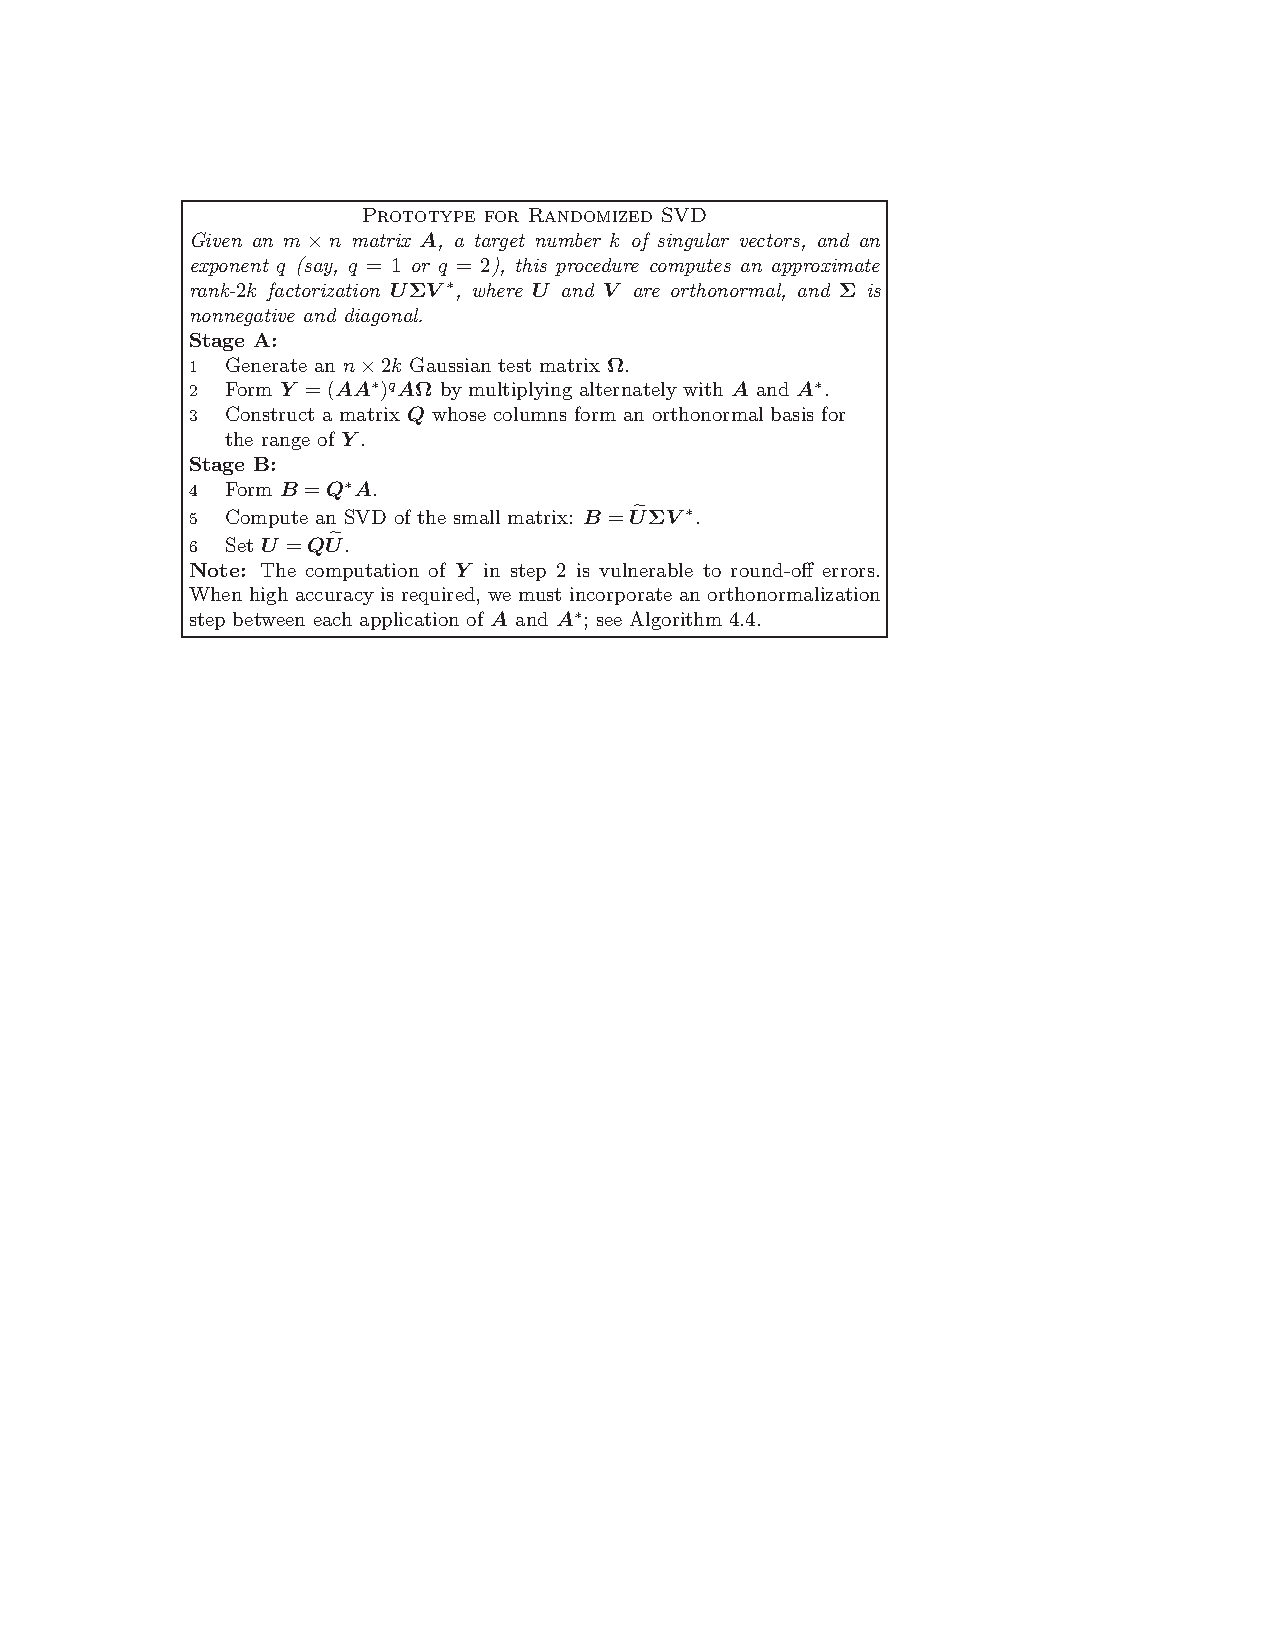
\includegraphics[width=.95\textwidth]{../common/pics/randSVDalg}
      \\
      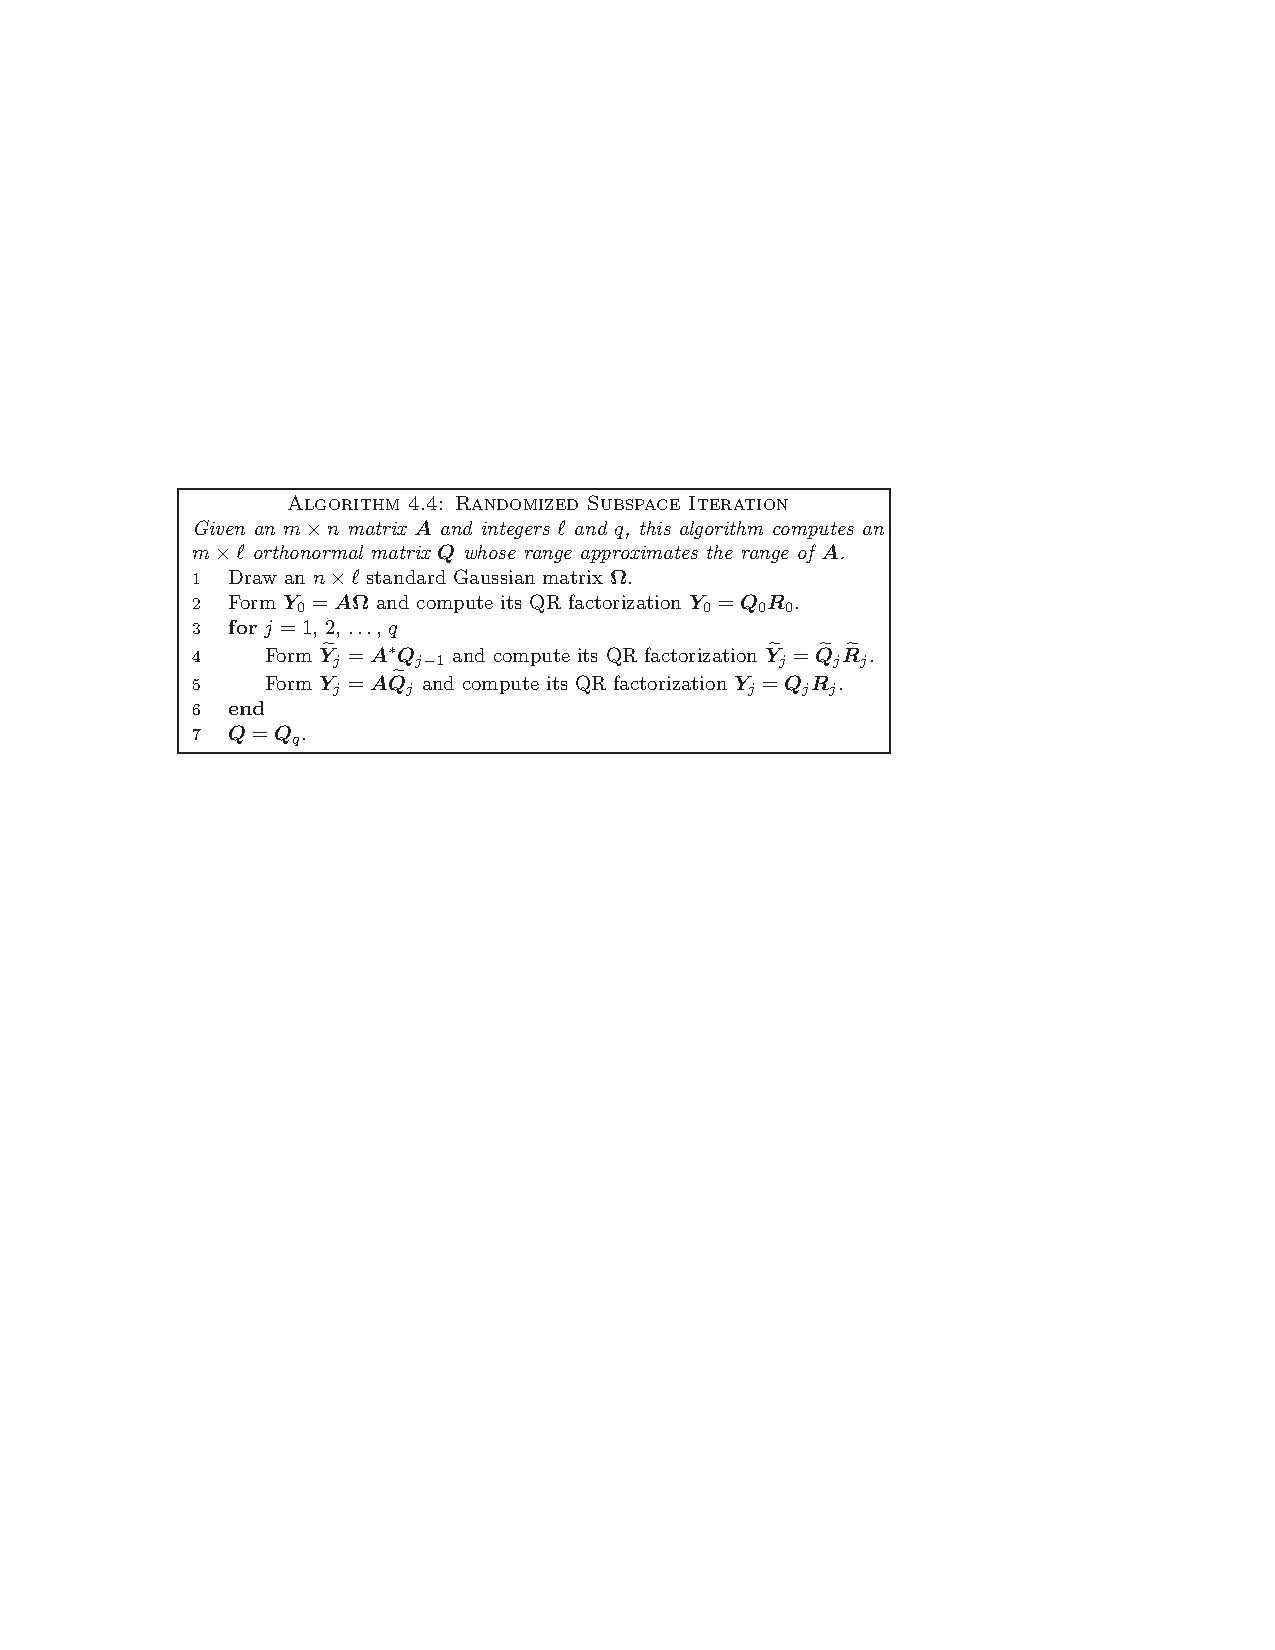
\includegraphics[width=.95\textwidth]{../common/pics/randSVDalg4_4}
    \end{center}
  \end{minipage}
%   \hspace{.01cm}
  \begin{minipage}{0.430\textwidth}
\begin{lstlisting}[title=Serial 
R,basicstyle=\tiny,backgroundcolor=\color{grayish} 
,numberstyle=\tiny\color{black},keywordstyle=\color{black},commentstyle=\color{ 
dkgreen},stringstyle=\color{black},escapeinside={(*@}{@*)}]
randSVD <- function(A, k, q=3)
  {
    ## Stage A
    Omega <- (*@ matrix(rnorm(n*2*k),@*) 
            (*@ nrow=n, ncol=2*k) @*)
    Y <- A %*% Omega
    Q <- qr.Q(qr(Y))
    At <- t(A)
    for(i in 1:q)
      {
        Y <- At %*% Q
        Q <- qr.Q(qr(Y))
        Y <- A %*% Q
        Q <- qr.Q(qr(Y))
      }
    
    ## Stage B
    B <- t(Q) %*% A
    U <- La.svd(B)$u
    U <- Q %*% U
    U[, 1:k]
  }
\end{lstlisting} %balance$
\end{minipage}
{\fontsize{6pt}{10}\selectfont $^1$Halko N, Martinsson P-G 
  and Tropp J A 2011 Finding structure with randomness: probabilistic algorithms 
  for constructing approximate matrix decompositions \emph{SIAM Rev.} \textbf{53} 
  217--88}
\end{block}
\end{frame}


\begin{frame}[fragile]
 \fontsize{8pt}{10}\selectfont
\begin{block}{Randomized SVD}
  \hfill
  \begin{minipage}{0.430\textwidth}
\begin{lstlisting}[title=Serial 
R,basicstyle=\tiny,backgroundcolor=\color{grayish} 
,numberstyle=\tiny\color{black},keywordstyle=\color{black},commentstyle=\color{ 
dkgreen},stringstyle=\color{black},escapeinside={(*@}{@*)}]
randSVD <- function(A, k, q=3)
  {
    ## Stage A
    Omega <- (*@ \textcolor{blue}{matrix(rnorm(n*2*k),} @*) 
         (*@ \textcolor{blue}{ nrow=n, ncol=2*k)} @*)
    Y <- A %*% Omega
    Q <- qr.Q(qr(Y))
    At <- t(A)
    for(i in 1:q)
      {
        Y <- At %*% Q
        Q <- qr.Q(qr(Y))
        Y <- A %*% Q
        Q <- qr.Q(qr(Y))
      }
    
    ## Stage B
    B <- t(Q) %*% A
    U <- La.svd(B)$u
    U <- Q %*% U
    U[, 1:k]
  }
\end{lstlisting} %balance$
  \end{minipage}
  \hfill
  \begin{minipage}{0.430\textwidth}
\begin{lstlisting}[title=Parallel pbdR,basicstyle=\tiny,backgroundcolor=\color{
grayish}, numberstyle=\tiny\color{black},keywordstyle=\color{black},
commentstyle=\color{dkgreen},stringstyle=\color{black},escapeinside={(*@}{@*)}]
randSVD <- function(A, k, q=3)
  {
    ## Stage A
    Omega <- (*@ \textcolor{blue}{ddmatrix("rnorm",} @*)
         (*@ \textcolor{blue}{nrow=n, ncol=2*k)} @*)
    Y <- A %*% Omega
    Q <- qr.Q(qr(Y))
    At <- t(A)      
    for(i in 1:q)
      {
        Y <- At %*% Q   
        Q <- qr.Q(qr(Y))
        Y <- A %*% Q    
        Q <- qr.Q(qr(Y))
      }
    
    ## Stage B
    B <- t(Q) %*% A     
    U <- La.svd(B)$u 
    U <- Q %*% U     
    U[, 1:k]
  }
\end{lstlisting}  % balancing $
  \end{minipage}
\hfill
\end{block}
\end{frame}

\begin{frame}
  \begin{block}{Randomized SVD}
    \begin{center}
      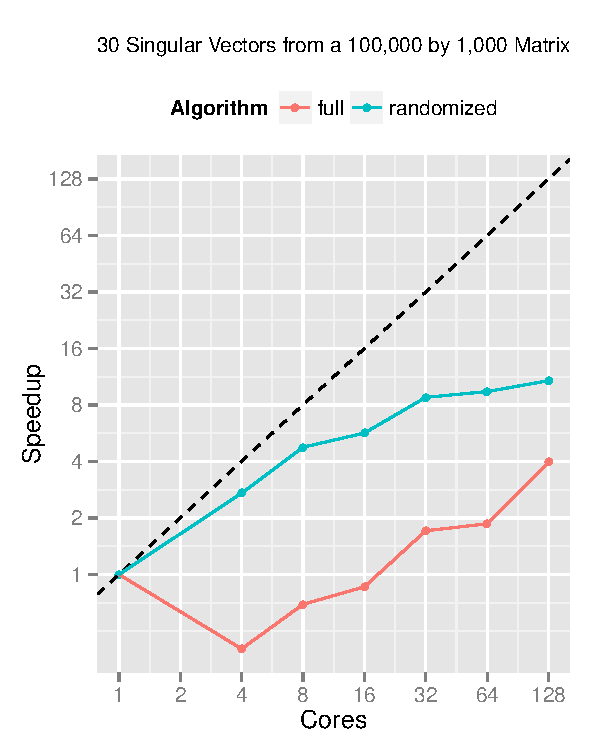
\includegraphics[width=.45\textwidth]{../common/pics/randSVDspeedup}
      \hfill
      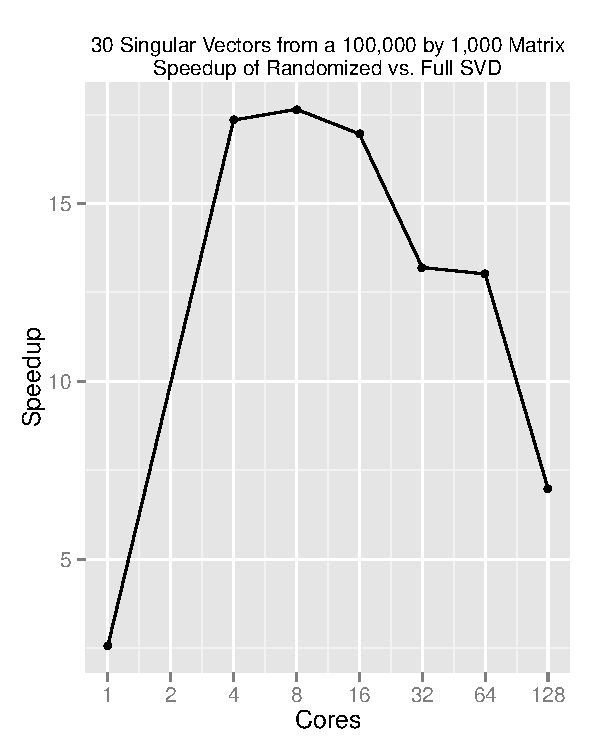
\includegraphics[width=.45\textwidth]{../common/pics/randSpeedupSVD}
    \end{center}
  \end{block}
\end{frame}
\begin{frame}
\frametitle{DMAT Exercises}
\begin{enumerate}
  \item Experiment with DMAT Examples 1 through 5, running them on 2 and 4 processors.
\end{enumerate}
\end{frame}



\begin{frame}[fragile,allowframebreaks=.9]
\frametitle{Advanced DMAT Exercises}
\begin{enumerate}
  \item  Subsetting, selection, and filtering are basic matrix operations featured
  in R. The following may look silly, but it is useful for data
  processing.  Let \code{x.dmat <- ddmatrix(1:30, 10, 3)}.  Do the following:
  \begin{itemize}
  \item
    \code{y.dmat <- x.dmat[c(1, 5, 4, 3), ]} \\
    \code{y.dmat <- x.dmat[c(10:3, 5, 5), ]} \\
    \code{y.dmat <- x.dmat[1:5, 3:1]}
  \\[.2cm]
  \item
    \code{y.dmat <- x.dmat[x.dmat[, 2] > 13, ]} \\
    \code{y.dmat <- x.dmat[x.dmat[, 2] > x.dmat[, 3], ]} \\
    \code{y.dmat <- x.dmat[, x.dmat[2,] > x.dmat[3, ]]} \\
    \code{y.dmat <- x.dmat[c(1, 3, 5), x.dmat[, 2] > x.dmat[, 3]]}
  \end{itemize}

  \item The method \code{crossprod()} is an optimized form of the crossproduct computation \code{t(x.dmat) \%*\% x.dmat}.  For this exercise, let \code{x.dmat <- ddmatrix(1:30, nrow=10, ncol=3)}.
  \begin{enumerate}
    \item Verify that these computations really do produce the same results.
    \item Time each operation.  Which is faster?
  \end{enumerate}

  \item The \code{prcomp()} method returns rotations for all components.  Computationally verify by example that these rotations are orthogonal, i.e., that their crossproduct is the identity matrix.

\end{enumerate}
\end{frame}
%%%%%%%%%%%%%%%%%%%%%%%%%%%%%%%%%%%%%%%%
%%     Last few slides
%%%%%%%%%%%%%%%%%%%%%%%%%%%%%%%%%%%%%%%%
\section{Wrapup}

\hidenum
\begin{frame}[noframenumbering]
\frametitle{Contents}
 \tableofcontents[currentsection,hideothersubsections,sectionstyle=show/hide]
\end{frame}
\shownum

\begin{frame}
  \begin{block}{Where to Learn More}
    \begin{itemize}
      \item Our website \url{http://r-pbd.org/}
      \item The \pkg{pbdDEMO} package\\
      \url{http://cran.r-project.org/web/packages/pbdDEMO/}\\
      \item The \pkg{pbdDEMO} Vignette: \url{http://goo.gl/HZkRt}
      \item Our Google Group: \url{http://group.r-pbd.org}
    \end{itemize}
\end{block}
\end{frame}


\section*{}


% \begin{frame}[fragile,allowframebreaks]
%   \tiny
%   \bibliographystyle{plainnat}
%   \bibliography{pbdbib}
% \end{frame}


\hidenum
\begin{frame}[noframenumbering]
 \begin{block}{Thanks for coming!}
 \begin{center}
     {\Large Questions?  Comments?}\\[.4cm]
     Please help us improve this tutorial by completing a short survey:\\
     \url{http://www.surveymonkey.com/s/W8VLJSP}
  \end{center}
 \end{block}
\end{frame}




\end{document}
%%%%%%%%%%%%%%%%%%%%%%%%%%%%%%%%